\subsection{Outline}
The systematics and cross-checks are presented in this section, with relative errors $\delta$ calculated in the following two scenarios:
\begin{itemize}
\item if one check is to compare with default: $\delta\equiv\frac{\mathcal{O}_\text{check}-\mathcal{O}_\text{default}}{\mathcal{O}_\text{default}}$;
\item if two checks (from sub-samples) are compared with each other: $\delta\equiv\frac{\mathcal{O}_\text{check 1}-\mathcal{O}_\text{check 2}}{\mathcal{O}_\text{check 1}+\mathcal{O}_\text{check 2}}$;
\end{itemize}
where $\mathcal{O}$ denotes the observable: 2-, 4- or 6-particle cumulant, and subscripts "default" and "check" are used to distinguish the different criteria.

The main systematic sources in this analysis are listed as follows:
\begin{itemize}
\item Monte-Carlo closure;
\item UCC trigger selection bias;
\item Loose v.s. tight track selection;
\item Low v.s. high tracking efficiency;
\item Impact of pileup rejection;
\item Flattening procedure;
\item Centrality definition;
\end{itemize}

The main cross-checks in this analysis are listed as follows:
\begin{itemize}
\item Event class bin width;
\item $\eta$ gap for subevent;
\end{itemize}

For simplicity, only systematics in standard cumulant are discussed, with following $p_{\text{T}}$ ranges:
\begin{itemize}
\item $c_1\{4\}$: $1.8<p_{\text{T}}<5.0$ GeV;
\item $c_2\{4\}$: $0.5<p_{\text{T}}<5.0$ GeV;
\item $c_3\{4\}$: $0.5<p_{\text{T}}<5.0$ GeV;
\item $c_4\{4\}$: $0.5<p_{\text{T}}<5.0$ GeV;
\end{itemize}
and for UCC trigger efficiency and pileup rejection, only systematics in ultra-central events are shown. At the end of this section, the summary of systematics are shown for all the observables.



\subsection{Ultra-central collision trigger efficiency}
In order to have enough statistics to study the cumulant in ultra-central collisions, ultra-central collision (UCC) triggered events are included. The trigger efficiencies are evaluated for all the UCC triggers separately. In the FCal $E_\text{T}$ region where trigger efficiency is less than 1 (turn-on region), due to the different tracking reconstructions between online and offline, event selection bias might be introduced to the analysis.

As one example, Fig.~\ref{fig:sys_trigEff_eg} shows the FCal $E_{T}$ distributions from MinBias and one of the UCC triggers: \verb|HLT_hi_|\verb|th1_ucc_L1TE10000| (left). This UCC trigger provides $~2$ times statistics than the MinBias trigger, in high FCal $E_{T}$ region, while the other UCC triggers provides more than 5 times statistics. The right plot shows the trigger efficiency. During the data taking, both MinBias and UCC triggers are heavily prescaled (except for the UCC triggers with highest threshold, which is running un-prescaled in most of the runs), and this means that the number of recorded events passing both MinBias and UCC triggers are extremely small. In order to evaluate the efficiency, we define the trigger "efficiency" on the statistical level:
\begin{equation}
\epsilon\equiv \frac{\sum\text{(event passing UCC * prescale)}}{\sum\text{(event passing MinBias trigger * prescale)}}
\end{equation}
Since the efficiency is defined on the statistical level, at large FCal $E_{T}$, the efficiency saturates towards 1, but not exactly at 1, as shown in the right plot of Fig.~\ref{fig:sys_trigEff}. Due to the strong correlation between online and offline FCal $E_{T}$, the turn-on curve of UCC triggers are very sharp, meaning that the selection bias due to UCC triggers are minimal. To be conservative, we still determined the FCal $E_{T}$ cut at $80\%$ efficiency for 3 sets of UCC triggers:
\begin{itemize}
\item FCal $E_{T}$ cut = 4.209 TeV for \verb|th1|;
\item FCal $E_{T}$ cut = 4.364 TeV for \verb|th2|;
\item FCal $E_{T}$ cut = 4.541 TeV for \verb|th3|;
\end{itemize}
\begin{figure}[H]
\centering
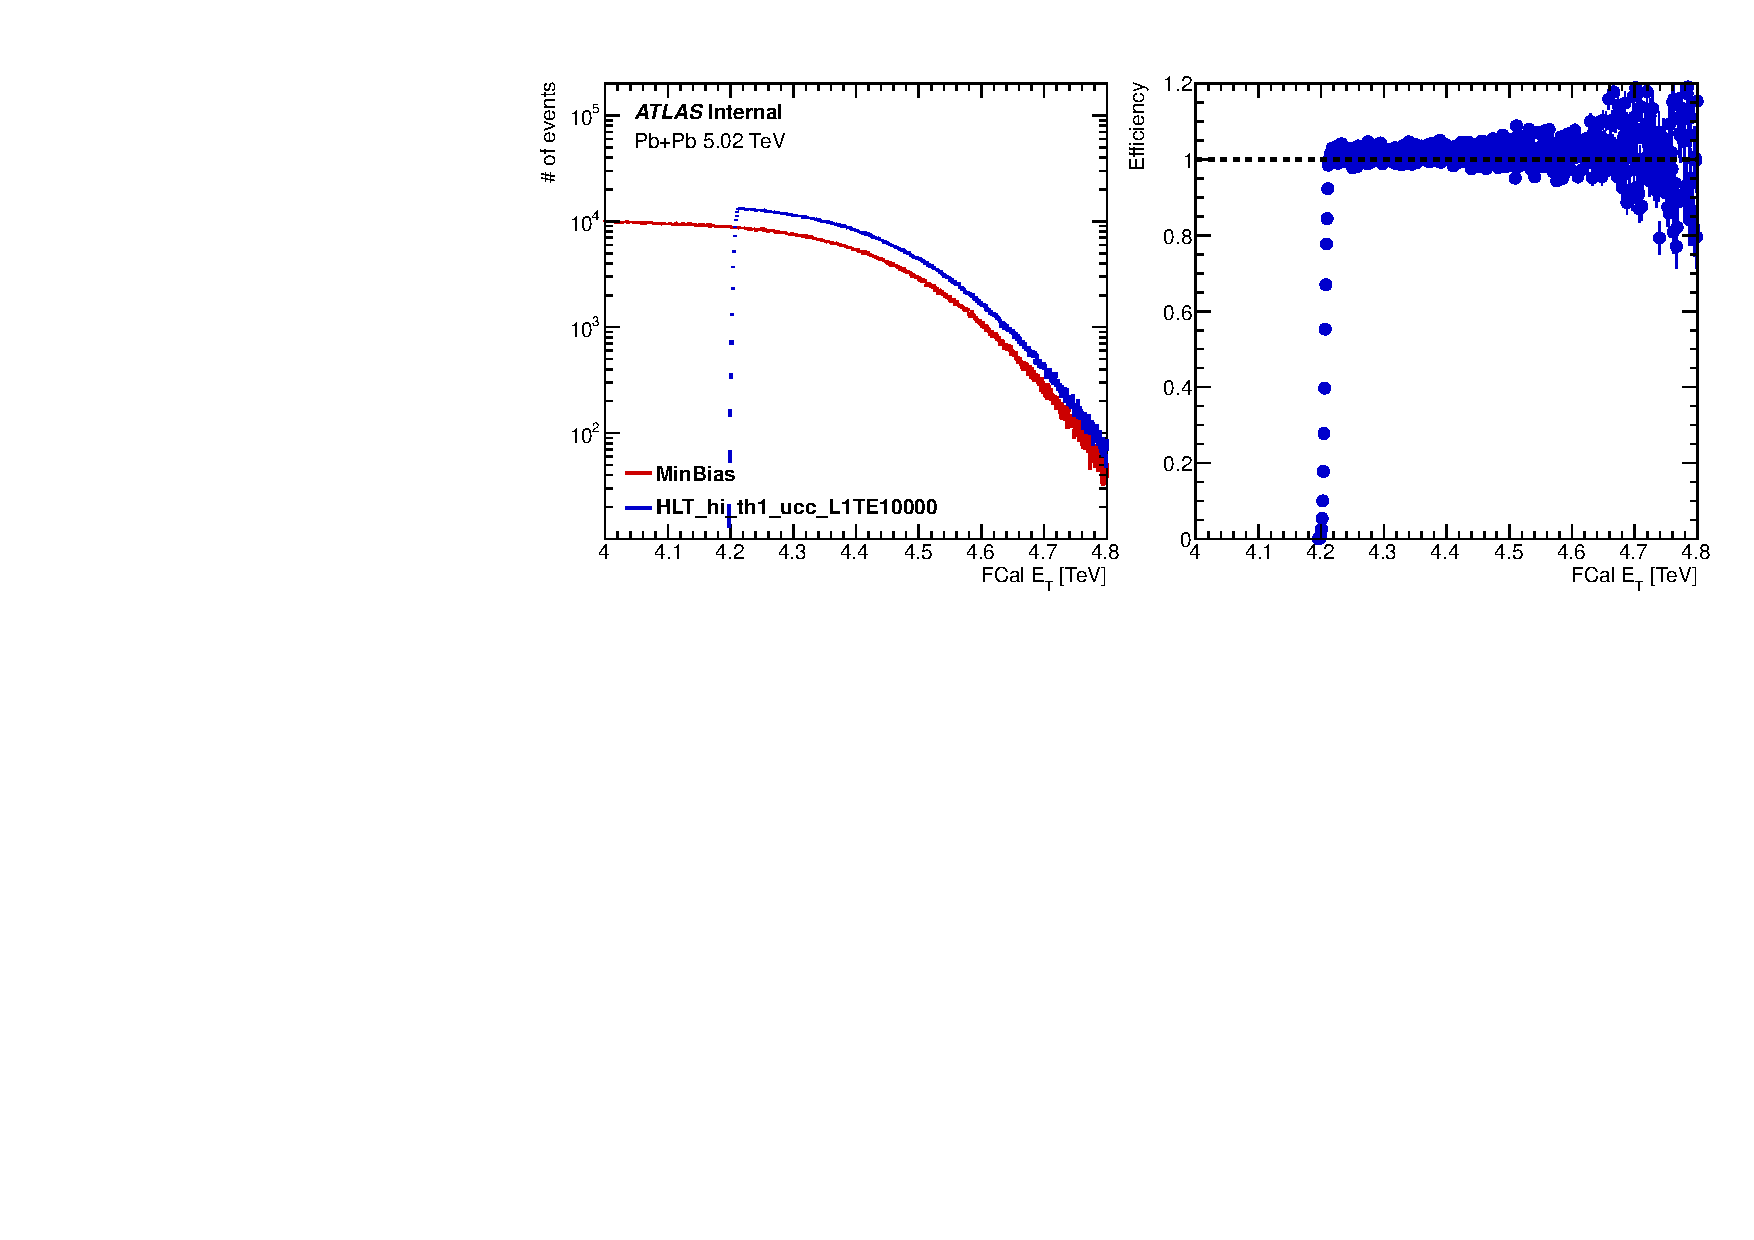
\includegraphics[width=.6\linewidth]{figs/sec_sys/trigEff_2.pdf}
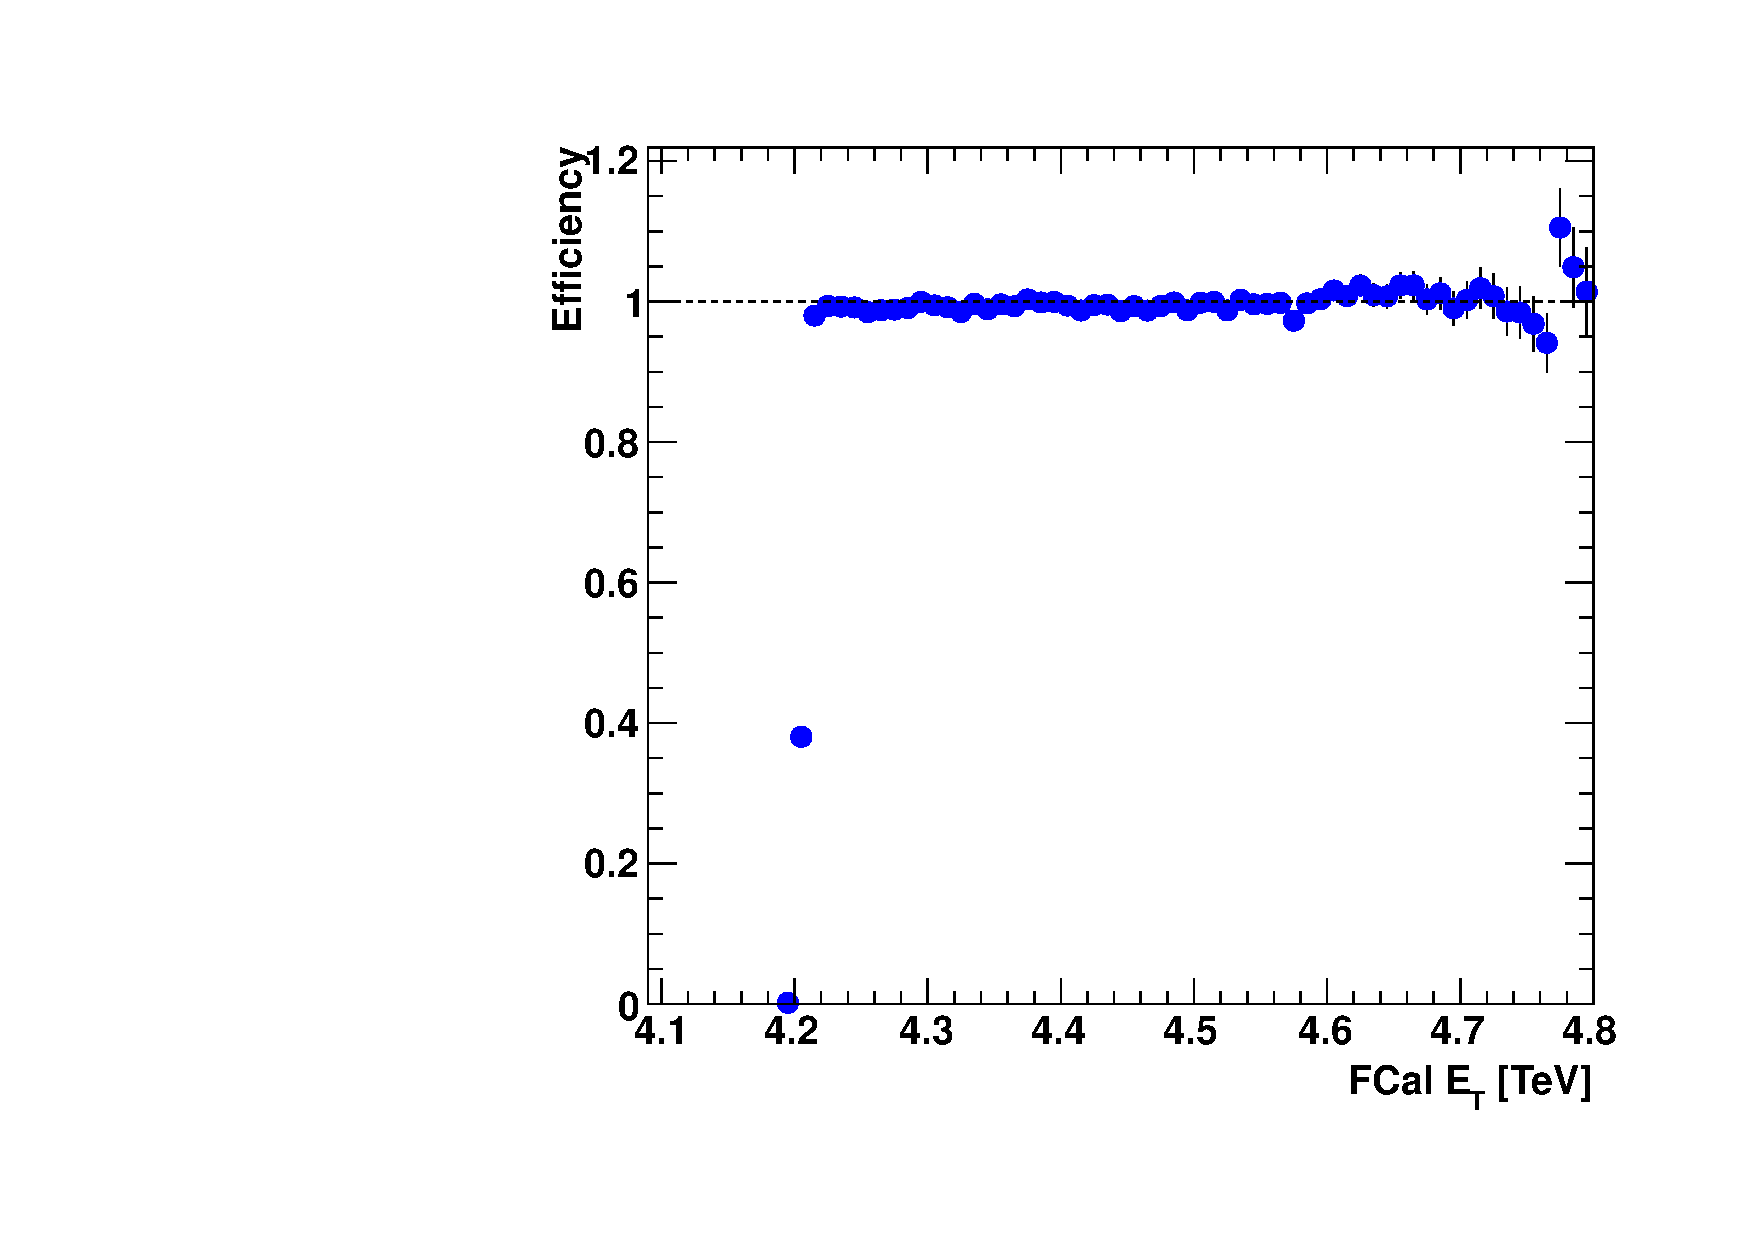
\includegraphics[width=.3\linewidth]{figs/sec_sys/trigEff_zoom.pdf}
\caption{$N_{ch}$ distributions from MinBias and one UCC trigger (left), trigger "efficiency" as a function of FCal $E_{T}$ (middle) and a zoomed-in version (right) to better see the plateau.}
\label{fig:sys_trigEff_eg}
\end{figure}

In order to evaluate the potential selection bias, we performed the following two checks:
\begin{itemize}
\item Default: include UCC events with efficiency higher than $80\%$;
\item Check: include all UCC events;
\end{itemize}

Fig.~\ref{fig:sys_trigEff} shows the comparison of $c_n\{4\}$ calculated with (default) and without (check) the trigger efficiency selection, as a function of FCal $E_{T}$ in central collision (Note UCC triggers have no impact on events with centrality $>1\%$). For all the four harmonics, the relative uncertainties are much smaller compared with statistical uncertainties. This is as expected because the turn-on curve of the trigger efficiency is very sharp: not many events are rejected because of the $80\%$ trigger efficiency selection.
\begin{figure}[H]
\centering
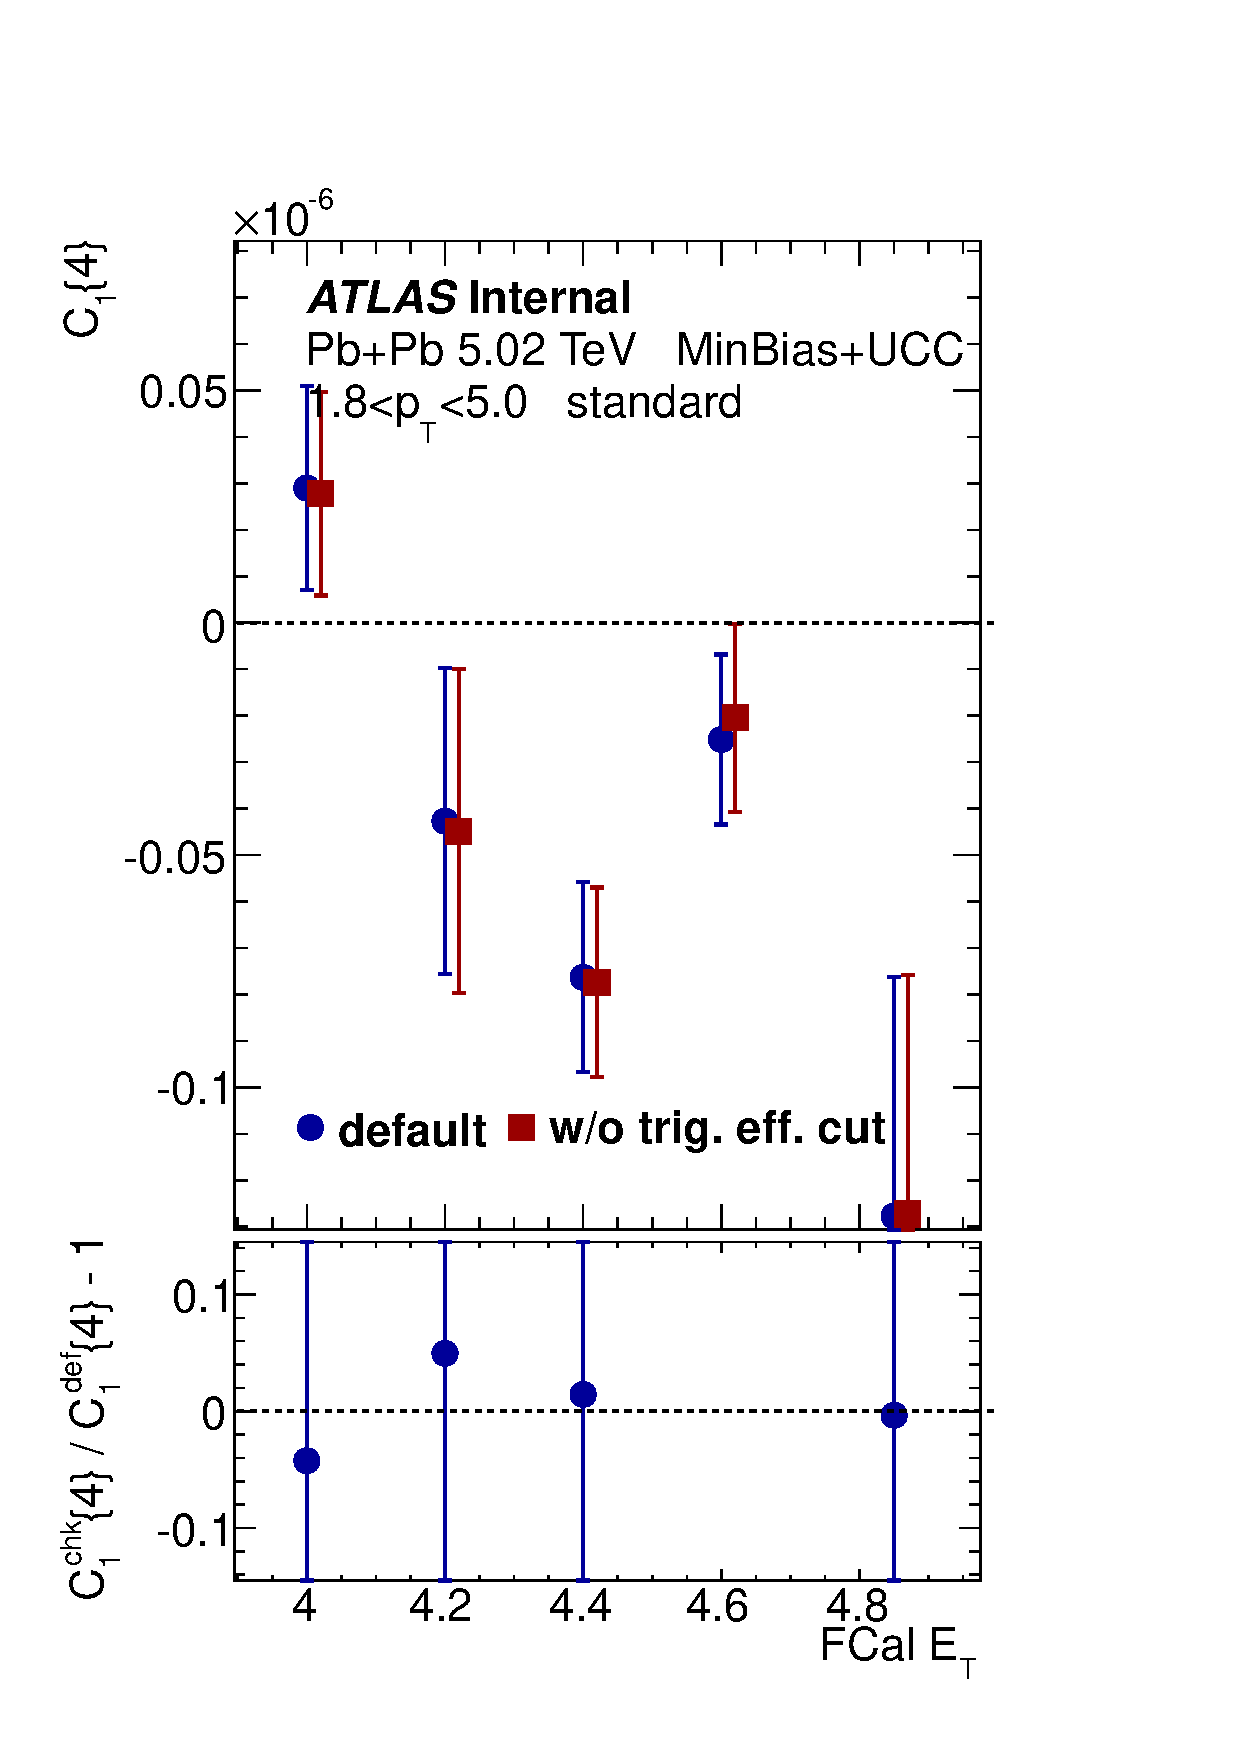
\includegraphics[width=.245\linewidth]{figs/sec_appendix/sys_PbPb502_UCC/PbPb502_sys12_1sub_Har1_Pt5.pdf}
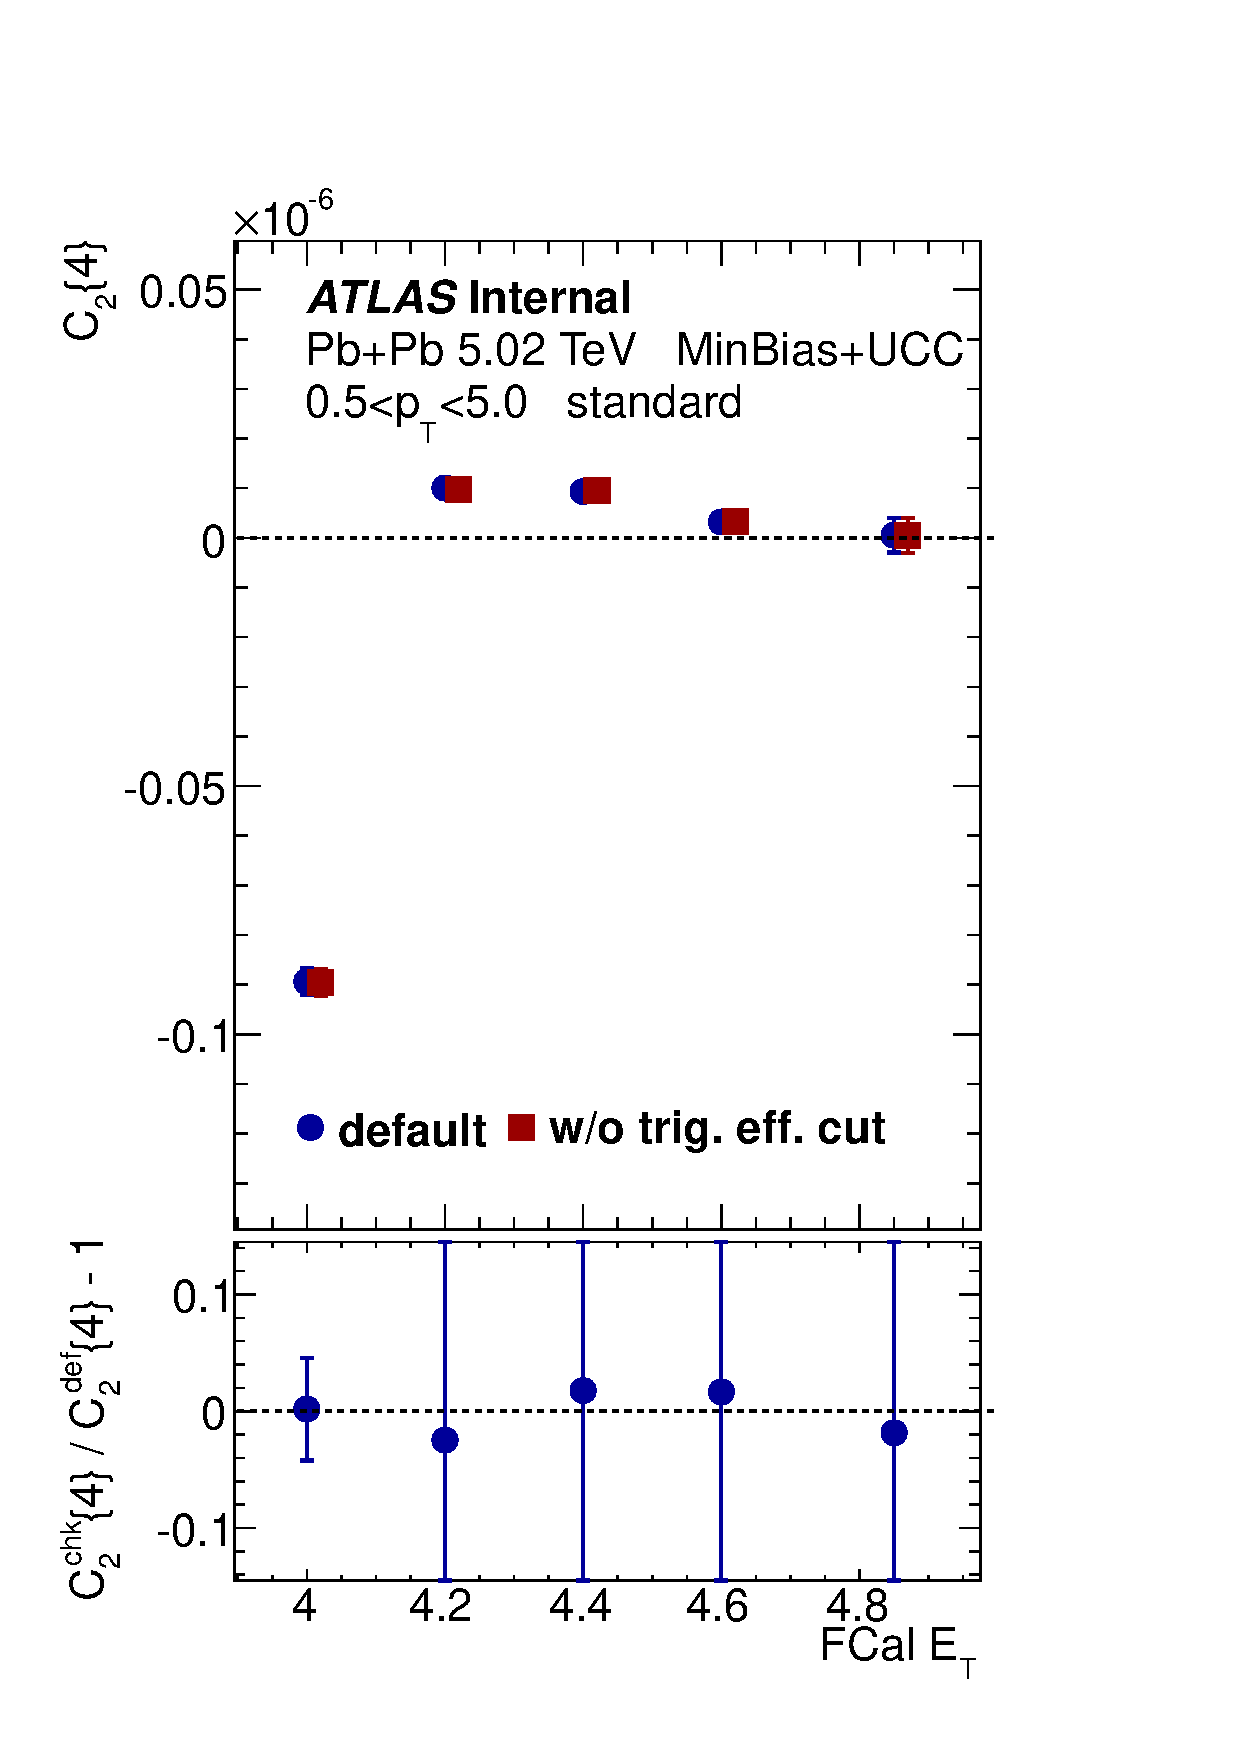
\includegraphics[width=.245\linewidth]{figs/sec_appendix/sys_PbPb502_UCC/PbPb502_sys12_1sub_Har2_Pt0.pdf}
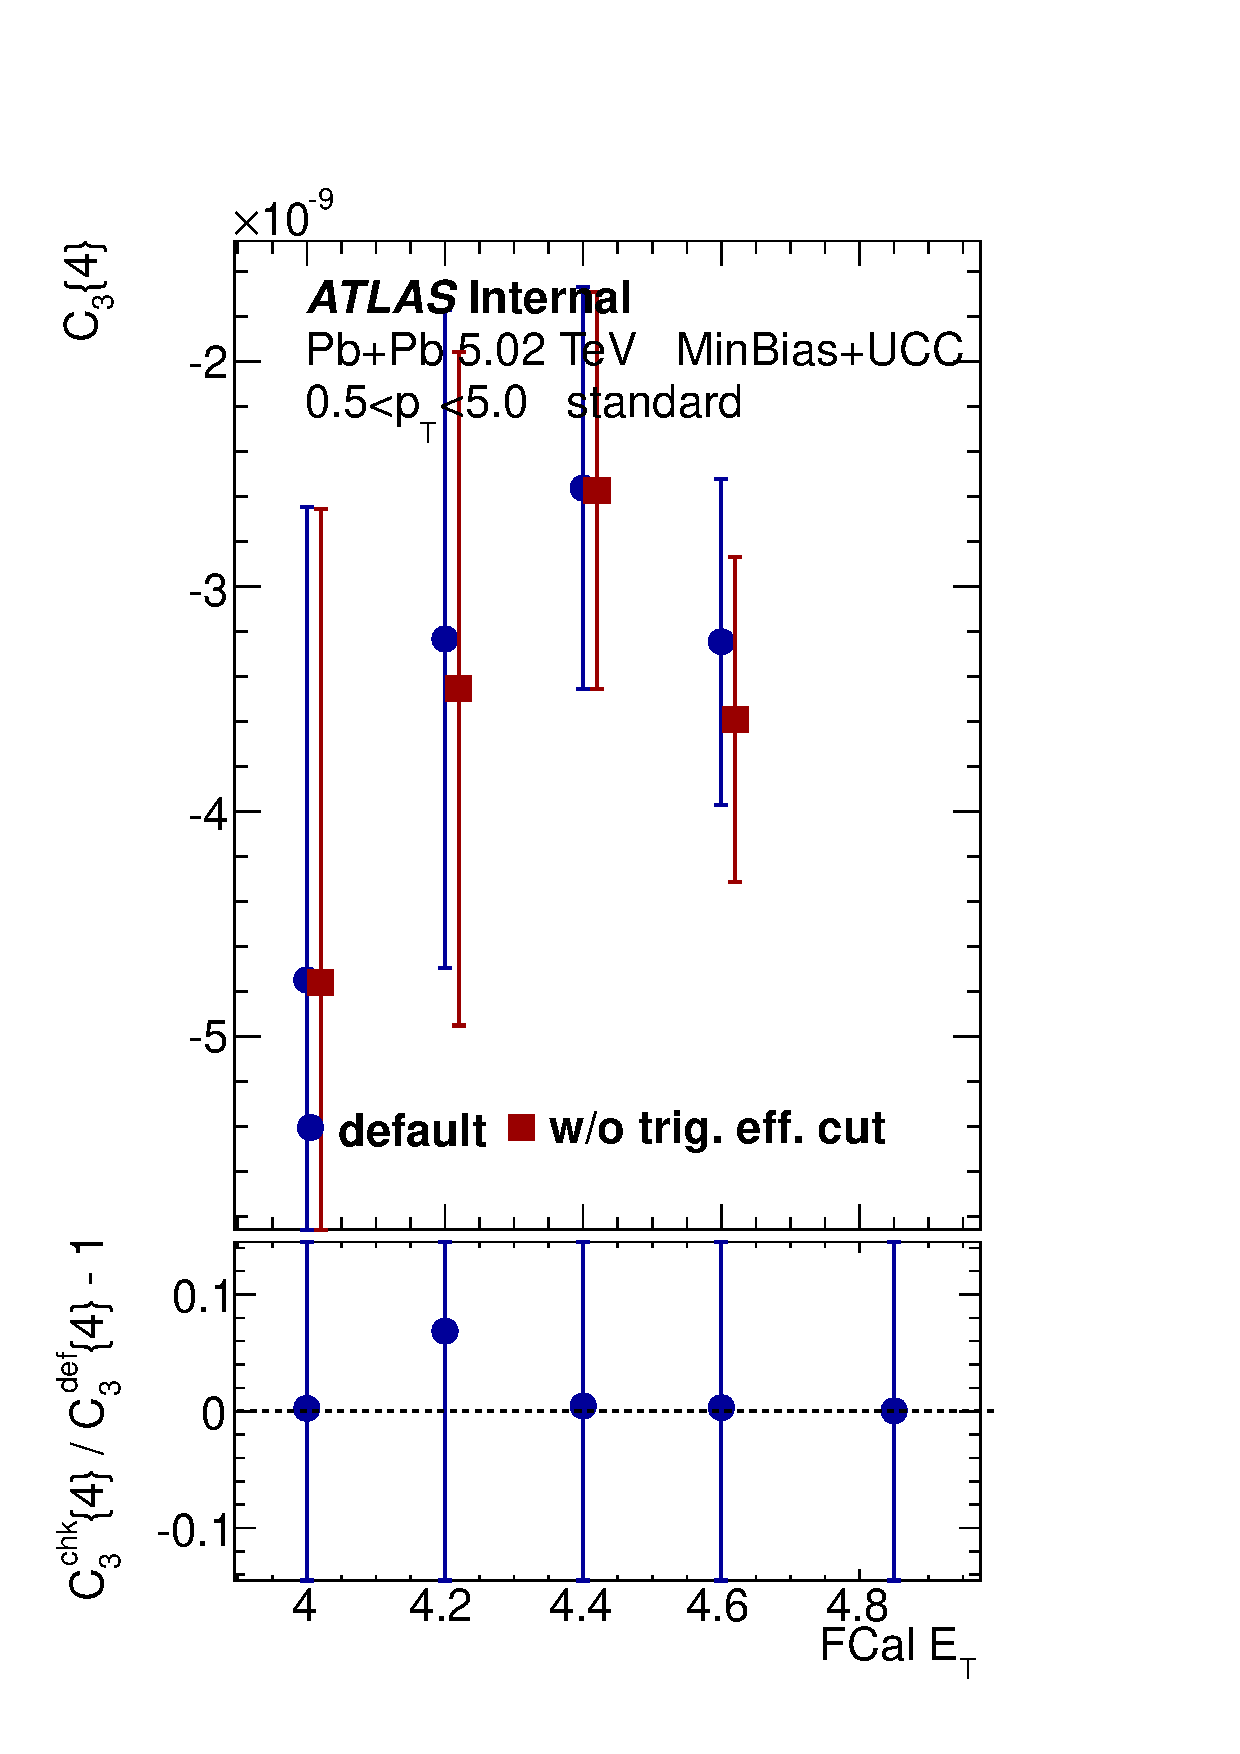
\includegraphics[width=.245\linewidth]{figs/sec_appendix/sys_PbPb502_UCC/PbPb502_sys12_1sub_Har3_Pt0.pdf}
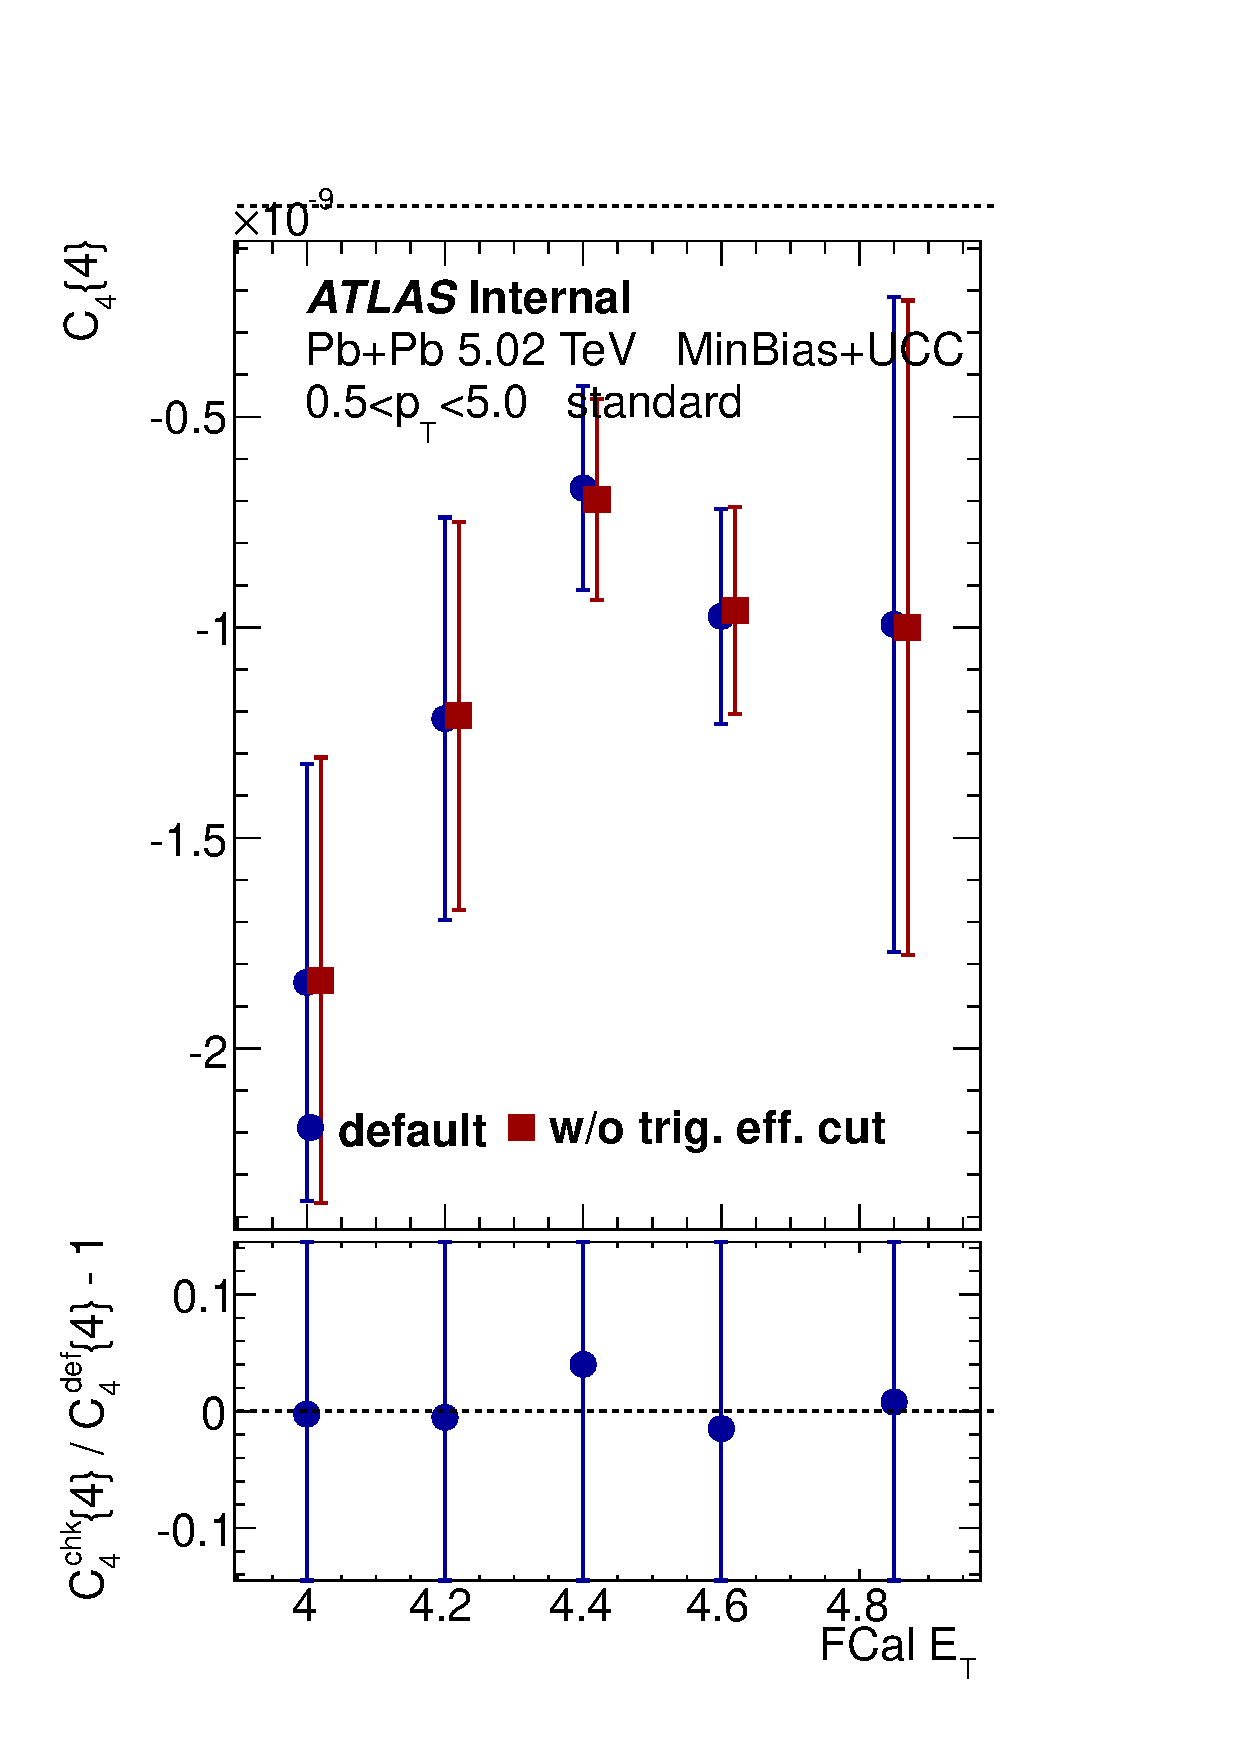
\includegraphics[width=.245\linewidth]{figs/sec_appendix/sys_PbPb502_UCC/PbPb502_sys12_1sub_Har4_Pt0.pdf}
\caption{Systematics of $c_n\{4\}$ from UCC trigger efficiency: with v.s. without trigger efficiency cut. Bottom panels are the relative uncertainties between the default and check.}
\label{fig:sys_trigEff}
\end{figure}

Due to much smaller systematic uncertainty compared with statistical uncertainty, trigger efficiency cut will not be quoted as part of the systematics.



\subsection{Monte-Carlo closure}
The HIJING Monte Carlo simulations were used to evaluate the difference between multi-particle cumulants in Pb+Pb data calculated using the generated and reconstructed charged particles obtained using the same analysis method. In some analysis it is considered as a crosscheck, since it assesses the quality of tracking, which are separately accounted for in previous systematics. The argument for not accounting it as a systematic uncertainties also relies on the fact that MC generators do not properly describe the investigated particle correlations. However, in this analysis, we are conservative to include the Monte-Carlo closure as part of the systematics.

Four million HIJING events with flow after-burner implemented are used for the MC closure (more details in \verb|ATLHI-116|). Note that both tracking and FCal $E_{T}$ are different between generated (truth) and reconstructed events, but in order to only evaluate the impact from offline tracking reconstruction, reconstructed FCal $E_{T}$, should be used for binning in both generated and reconstructed. Otherwise the differences between generated and reconstructed FCal $E_{T}$ will convolute with the tracking reconstruction, and that is not the purpose of this systematic check. However, the Monte-Carlo samples are generated using fast MC simulation configurations, which creates discrepancy of Calorimeter $E_{T}$ between data and MC. Due to this reason, the closure test was first binned in $N_{ch}^{rec}$, which is consistent with data, then mapped to the FCal $\lr{E_T}$ of data. In this case, the mismatch of FCal $E_{T}$ between data and MC plays little role. The procedure is similar as the Run 2 $v_n$ analysis~\cite{Burka:2151932}.

For the reconstructed tracks, it is not required to be associated with truth track, and both efficiency and fake rates are needed for the correction. Meanwhile, we do observe that the average of $\phi$ distribution is not very uniform in reconstructed tracks due to the simulation of detector effects, so flattening procedure is also applied in this Monte-Carlo check. In summary, all the corrections that has been applied in data analysis are also repeated with the Monte-Carlo test.

Fig.~\ref{fig:sys_mc} shows the $c_n\{4\}$ calculated from generated and reconstructed particles. Since the HIJING sample has flow implemented, both $c_2\{4\}$ and $c_3\{4\}$ show similar centrality dependence as data: largest in mid-central and approaches $0$ in central and peripheral. The relative differences are largest in central: reaching $3\%$, even after the efficiency and fake corrections are applied to the reconstructed tracks. As to $c_1\{4\}$ and $c_4\{4\}$, the centrality dependence is very different compared with data and the statistical errors are quite large. Due to these reasons, relative differences for $c_1\{4\}$ and $c_4\{4\}$ are not quoted as part of the systematics.
\begin{figure}[H]
\centering
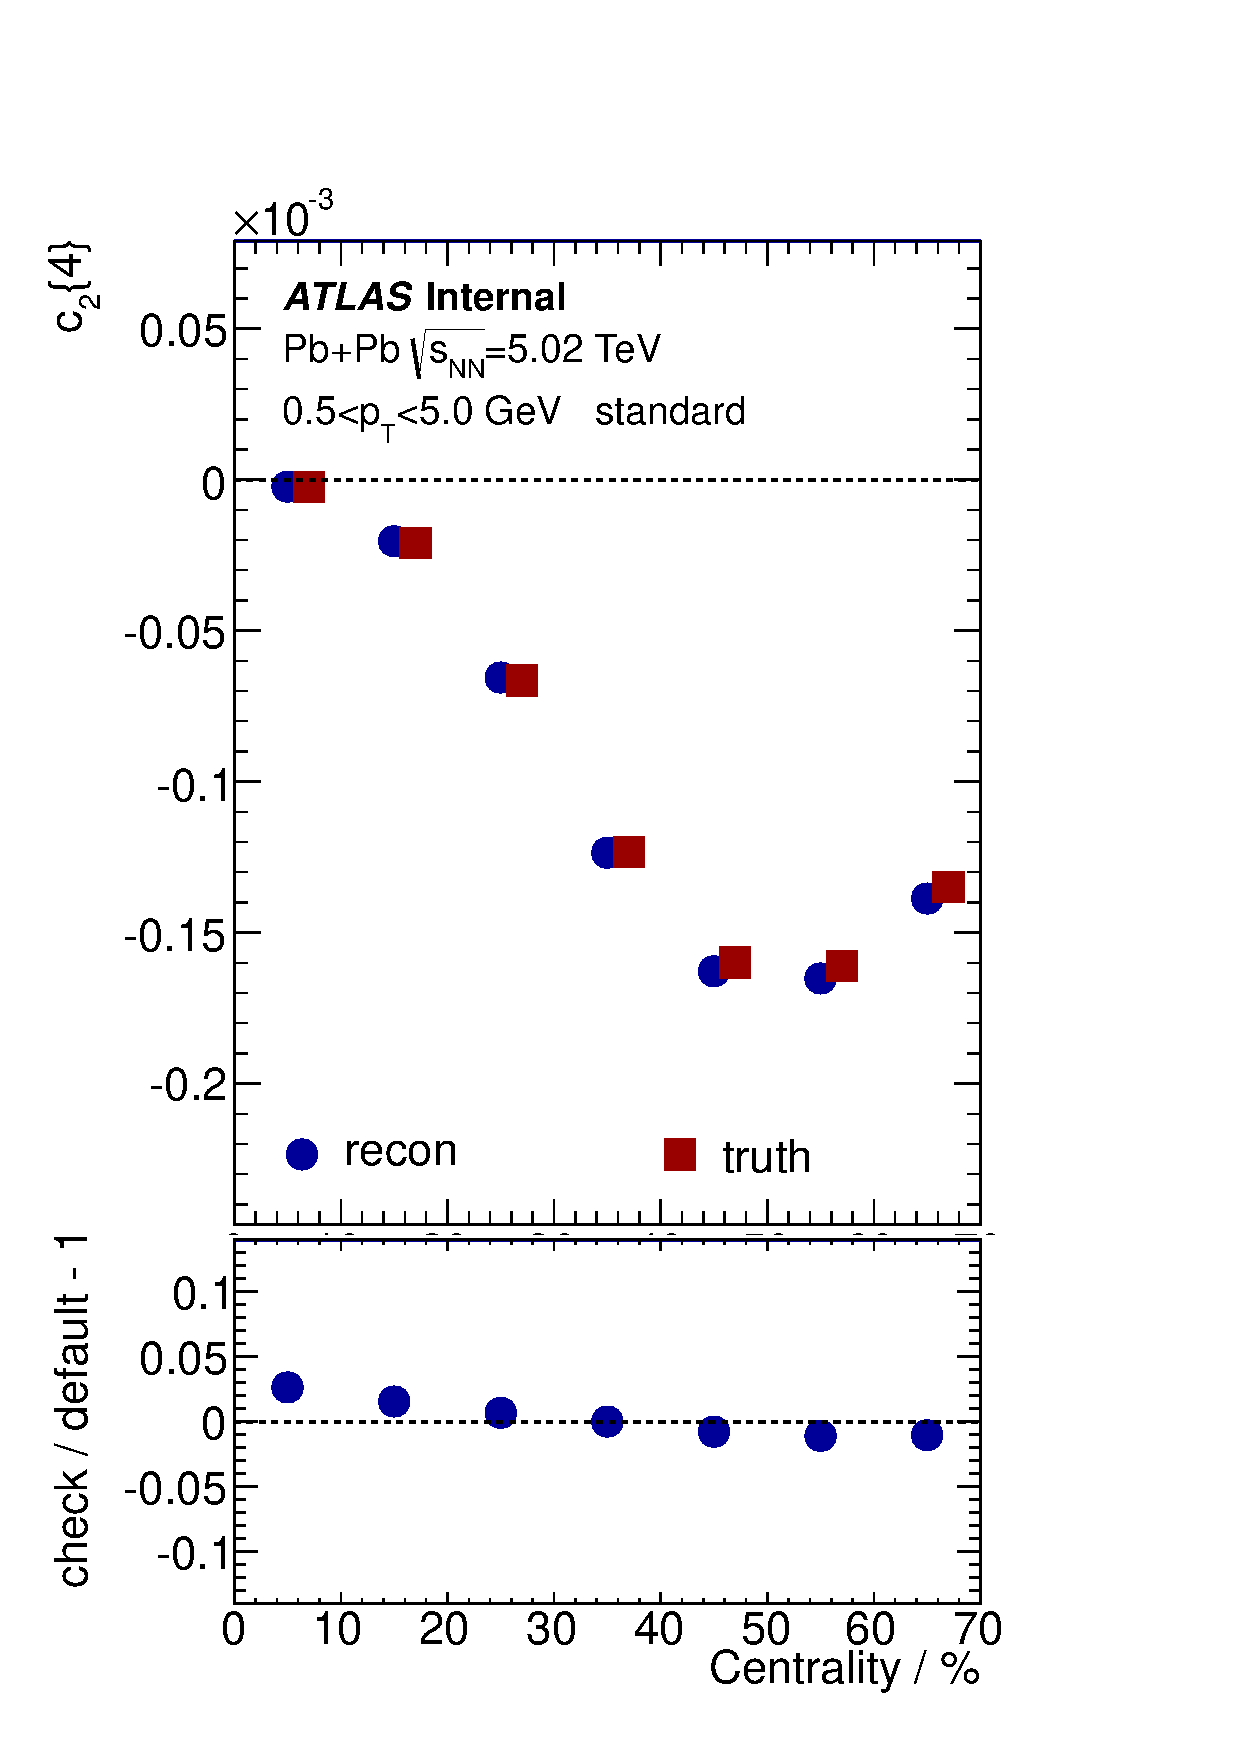
\includegraphics[width=.245\linewidth]{figs/sec_sys/summary/sys5_c4_1sub_Har2_Pt0.pdf}
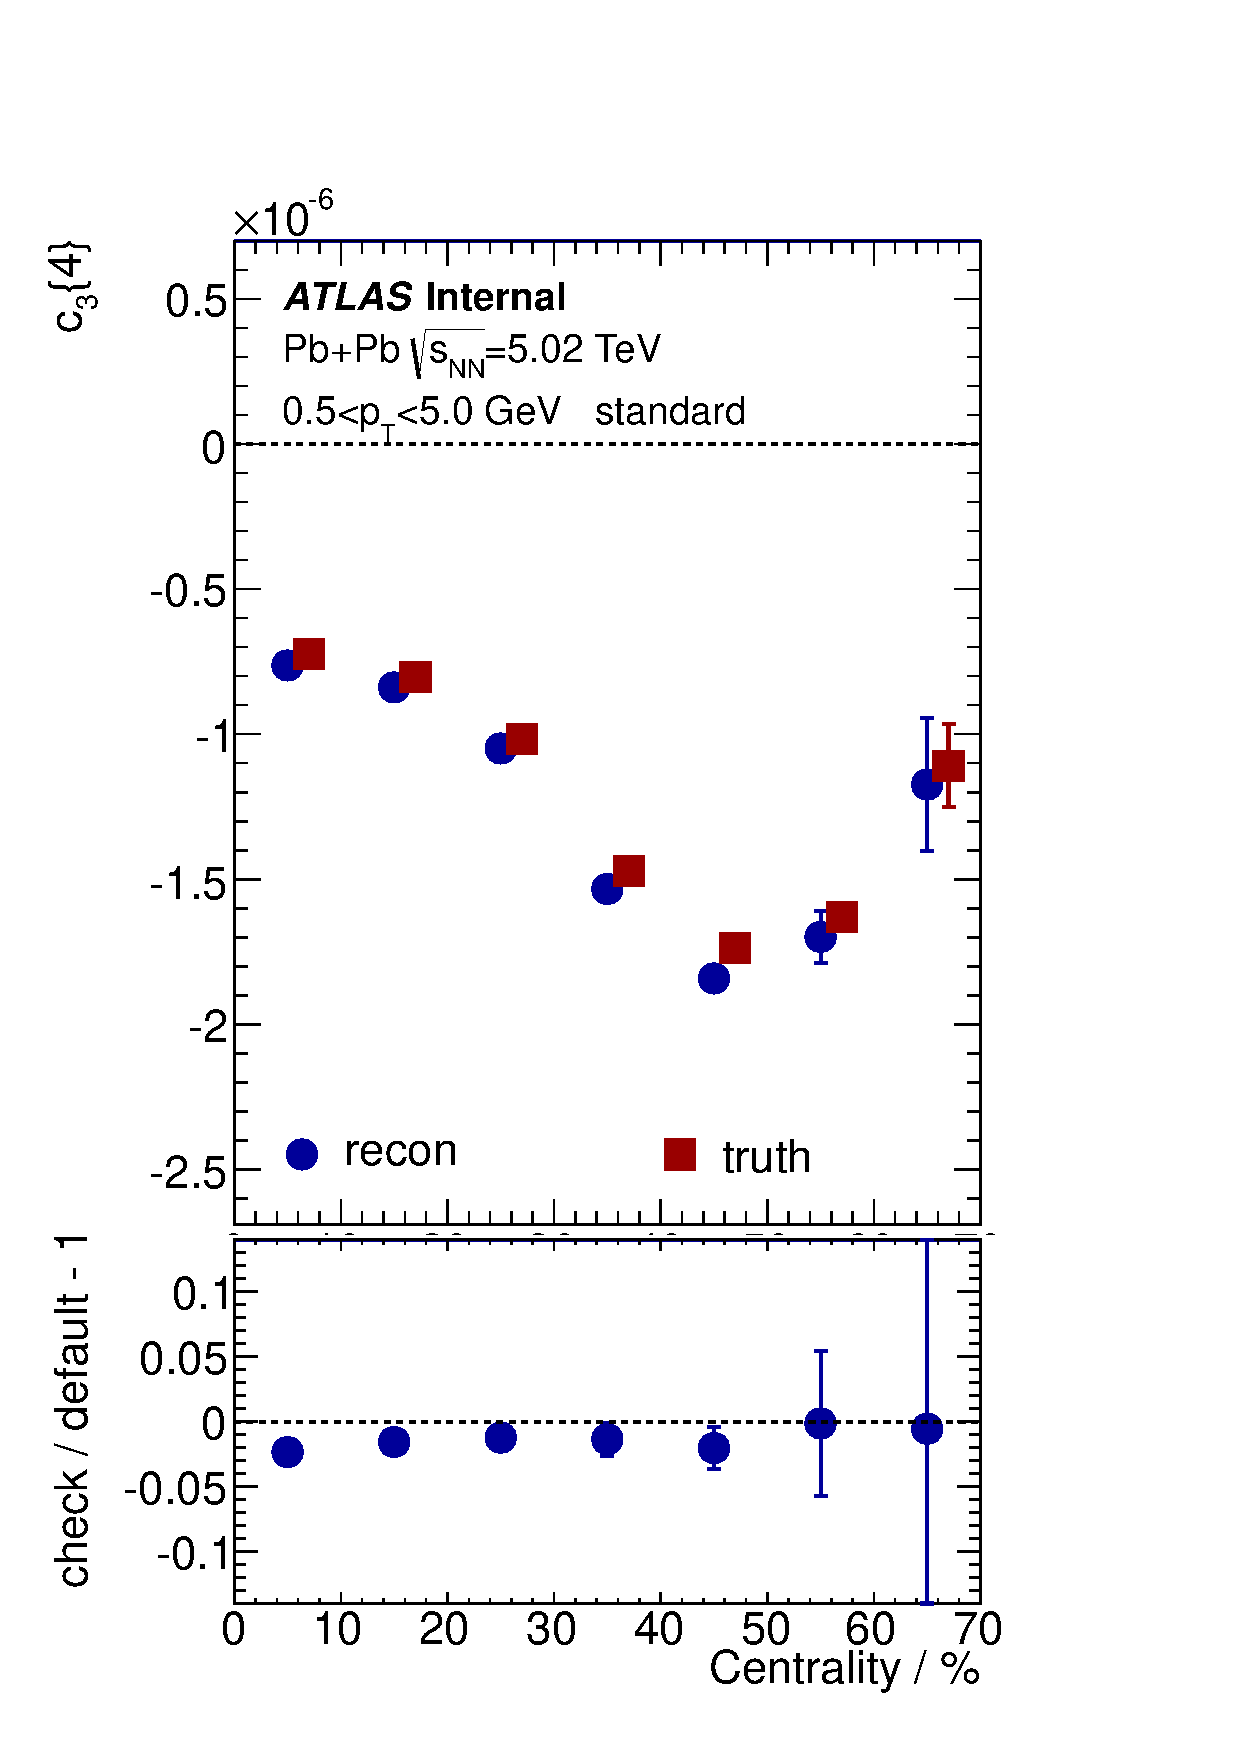
\includegraphics[width=.245\linewidth]{figs/sec_sys/summary/sys5_c4_1sub_Har3_Pt0.pdf}
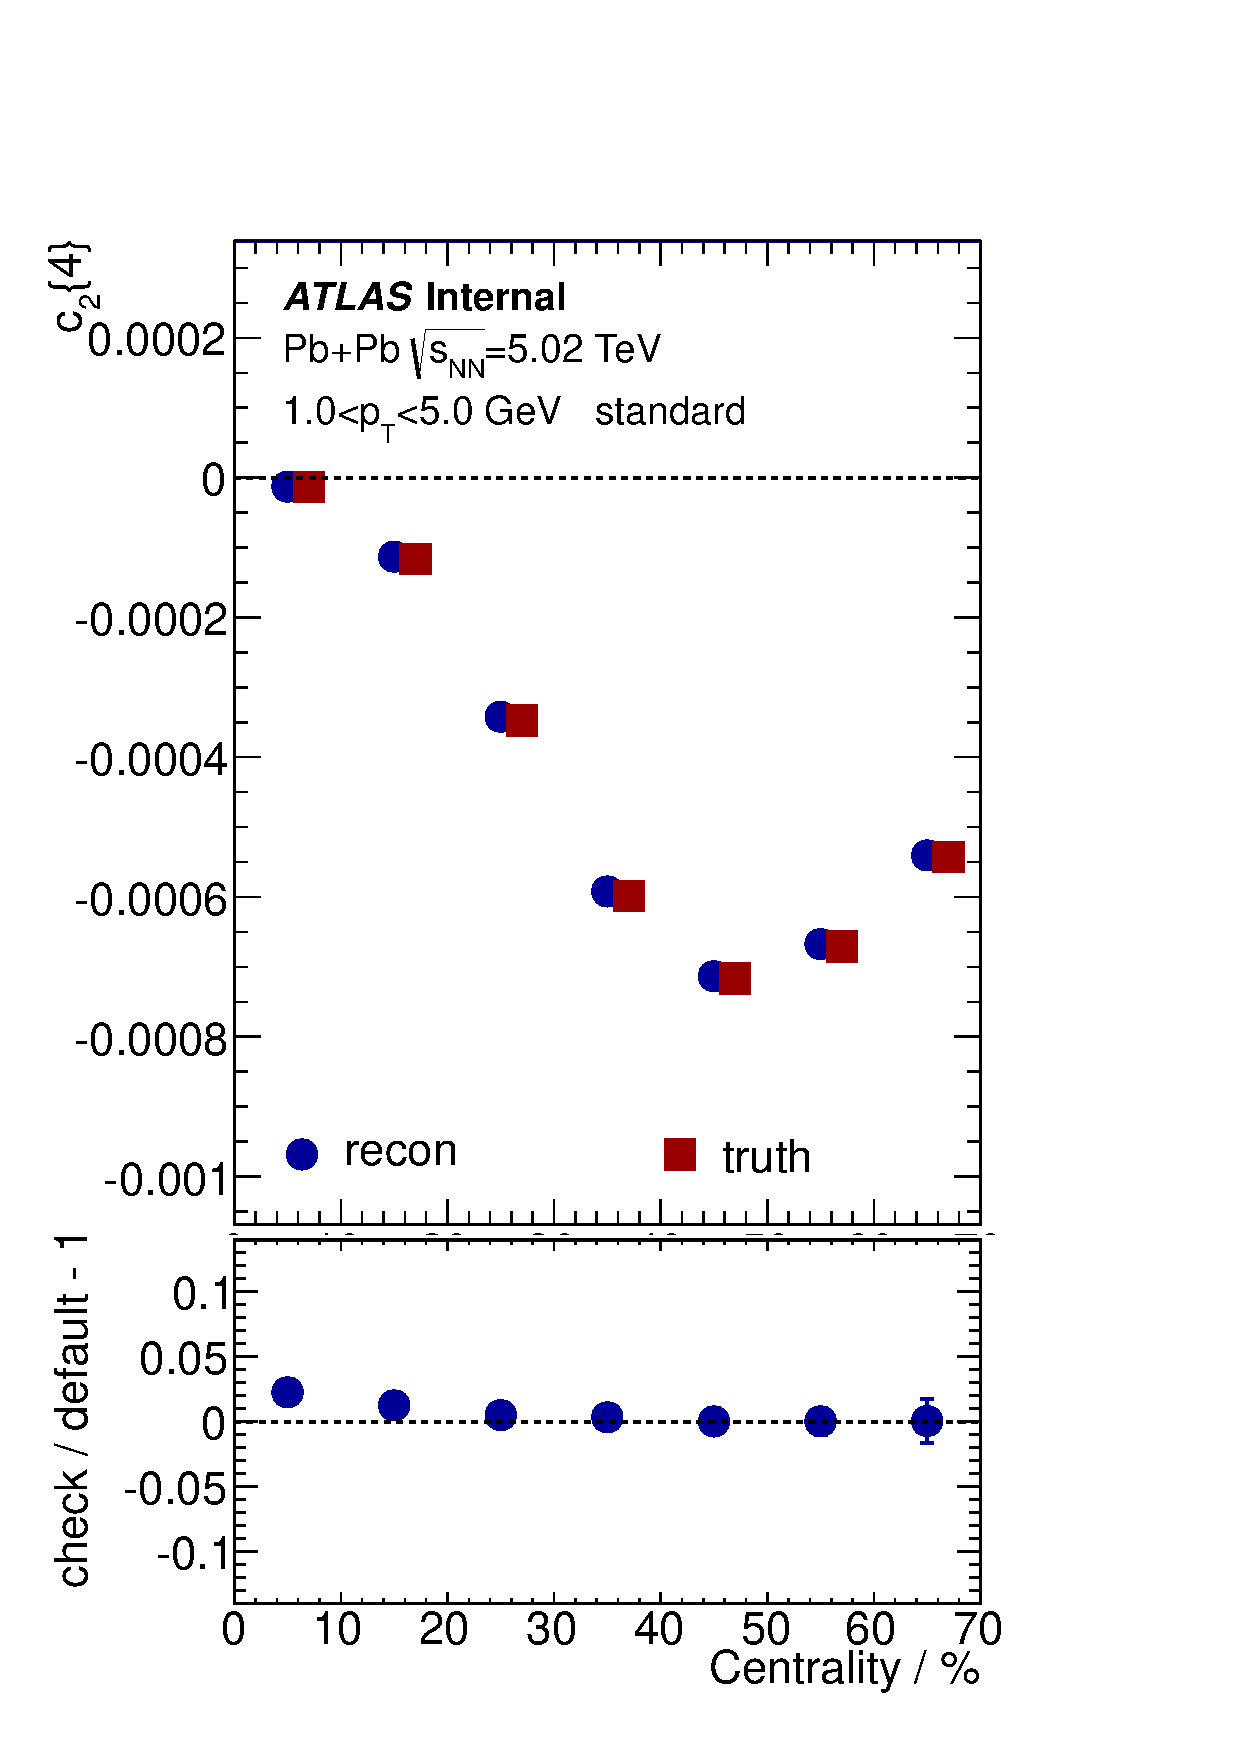
\includegraphics[width=.245\linewidth]{figs/sec_sys/summary/sys5_c4_1sub_Har2_Pt1.pdf}
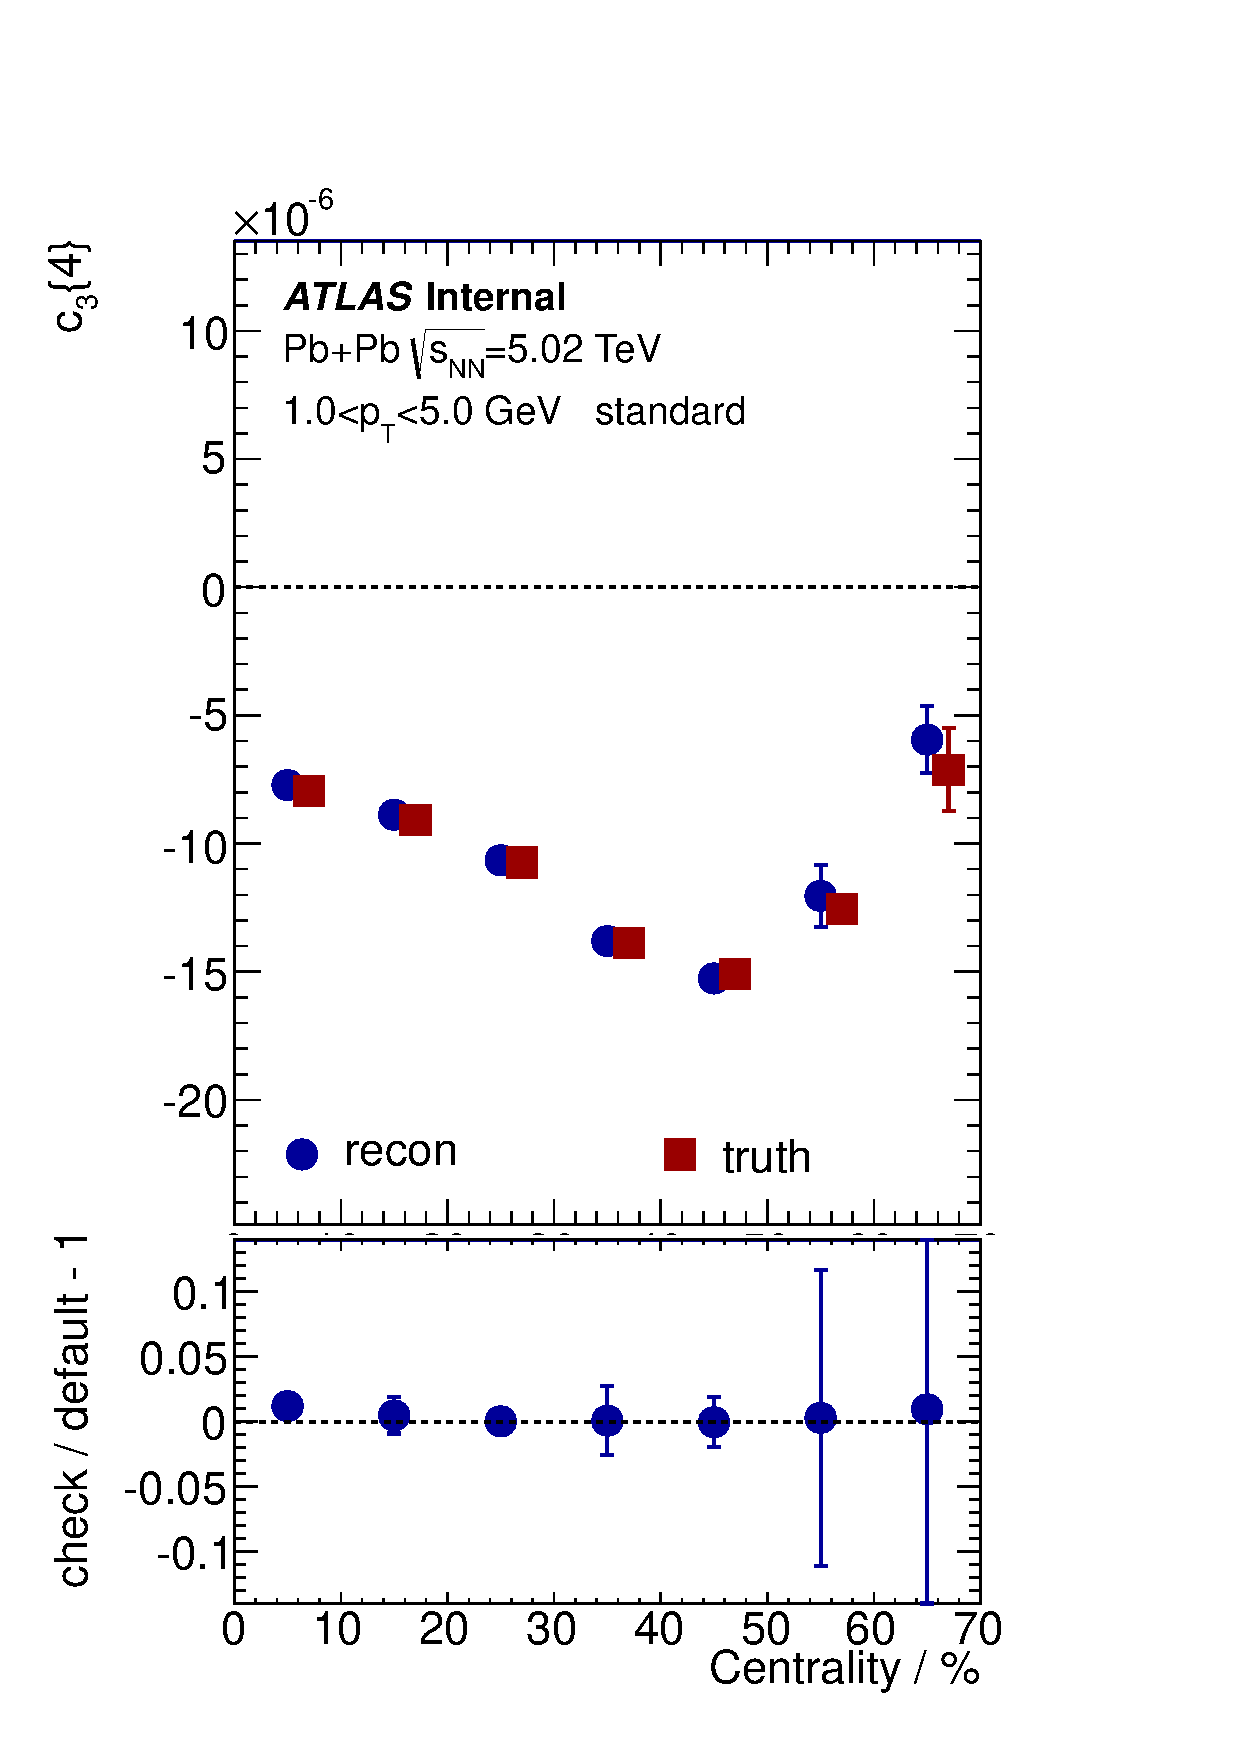
\includegraphics[width=.245\linewidth]{figs/sec_sys/summary/sys5_c4_1sub_Har3_Pt1.pdf}
\caption{Systematics of $c_n\{4\}$ from MC closure: generated v.s. reconstructed. Bottom panels are the relative uncertainties between the default and check. Note that the relative difference for $c_1\{4\}$ and $c_4\{4\}$ are set to be 0 (see main text).}
\label{fig:sys_mc}
\end{figure}

In addition, we have tested the following checks trying to diminish the $10\%$ differences observed in $c_2\{4\}$ and $c_3\{4\}$:
\begin{itemize}
\item Using a different 0.5 million HIJING sample (see in \verb|ATLHI-84|): similar outcome;
\item Do not apply efficiency or fake correction to reconstructed tracks: larger difference;
\item Only apply tracking efficiency: larger difference in central;
\item Apply flattening procedure on reconstructed tracks: similar outcome;
\item Apply additional $d_0$ and $z_0$ significance cuts to reconstructed tracks: larger difference;
\end{itemize}
Unfortunately, average efficiency and fake corrections will not compensate the inefficiency of reconstruction of tracks. To be conservative, the relative differences are quoted as systematics for both $c_2\{4\}$ and $c_3\{4\}$. As to the systematics in ultra-central collisions, since this HIJING sample does not contain enough ultra-central events, the systematic errors in UCC events are quoted from the plots above (error from the most central bin).

Since HIJING simulation does not implement correlation between flow harmonics, as shown in Fig.~\ref{fig:sys_mc_sc}(the signals are much smaller compared with data), systematics from MC closure for symmetric and asymmetric cumulant are set to be 0.
\begin{figure}[H]
\centering
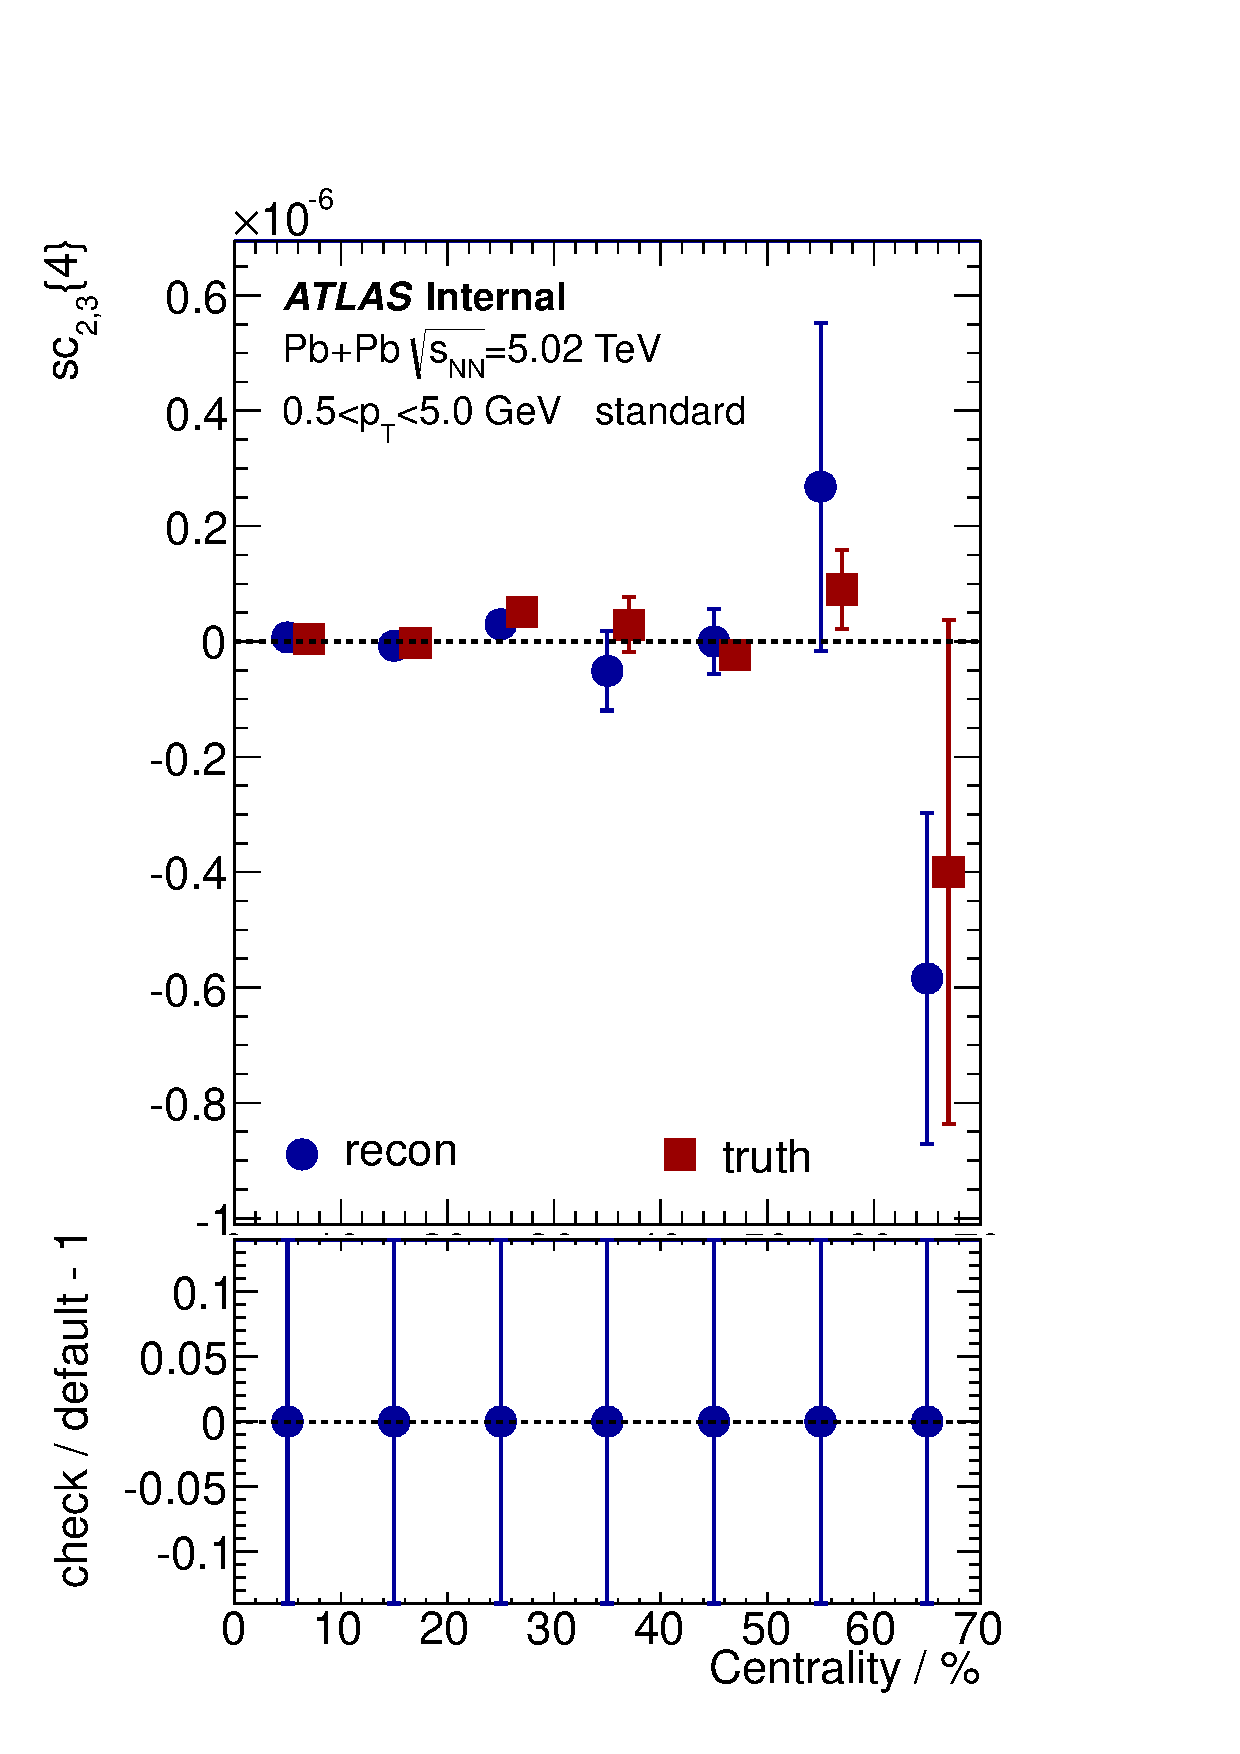
\includegraphics[width=.245\linewidth]{figs/sec_sys/summary/sys5_sc_1sub_Har2_Pt0.pdf}
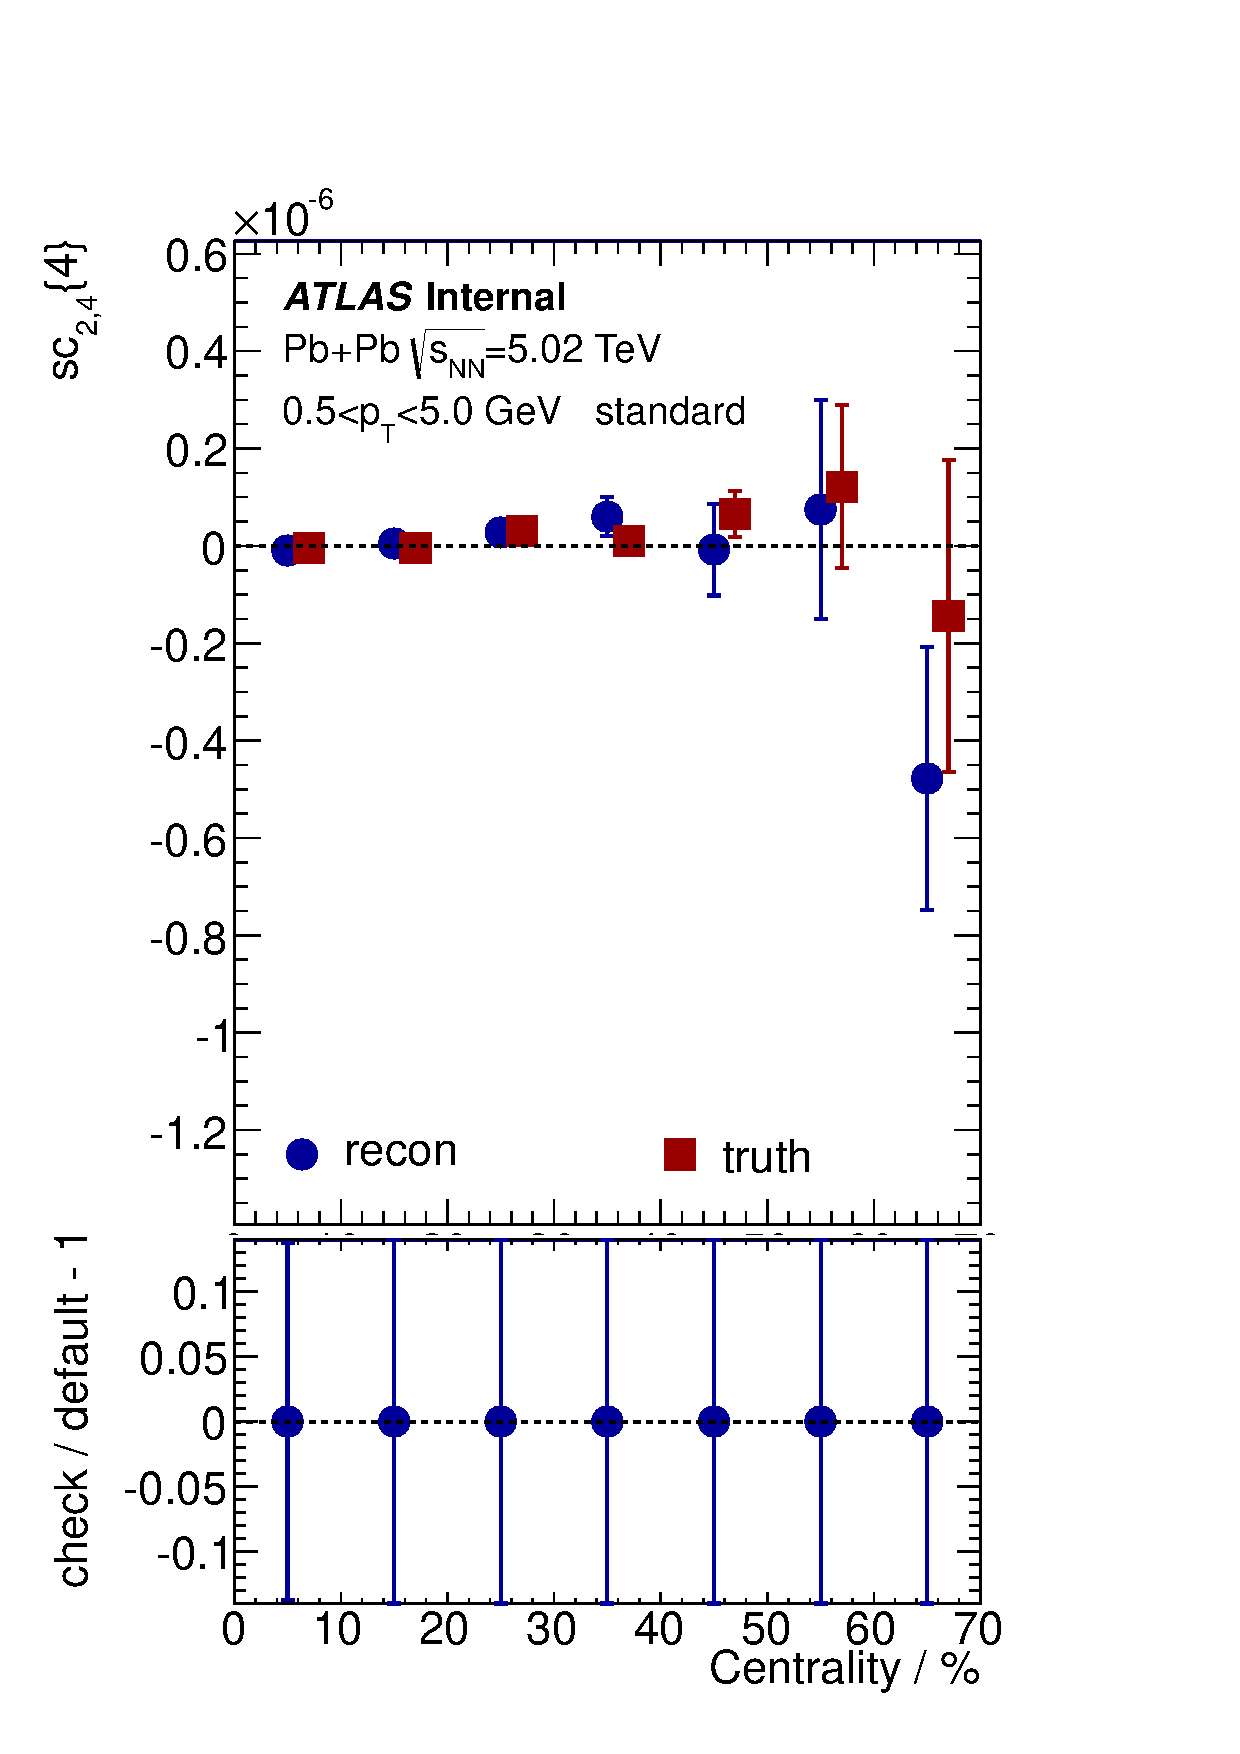
\includegraphics[width=.245\linewidth]{figs/sec_sys/summary/sys5_sc_1sub_Har3_Pt0.pdf}
\caption{Systematics of symmetric cumulants from MC closure: generated v.s. reconstructed. Bottom panels are the relative uncertainties between the default and check. Note that the relative differences are set to be 0 (see main text).}
\label{fig:sys_mc_sc}
\end{figure}



\subsection{Loose and tight track selection}
As default, the heavy ion loose track quality cut is applied in this analysis. In order to check stability of the track selection cuts, analysis is also repeated with tight track quality cut:
\begin{itemize}
\item Default: HI loose quality cut;
\item Check: HI tight quality cut;
\end{itemize}
where the definitions of loose and tight are listed in Section.~\ref{sec:trkSel}.

Fig.~\ref{fig:sys_trkSel} compares the $c_n\{4\}$ calculated with HI loose and tight track selection. For $c_2\{4\}$ and $c_3\{4\}$, the relative differences are within $3\%$ for all centralities. While for $c_1\{4\}$ and $c_4\{4\}$, since the signal is much smaller, the relative errors go up to $10\%$, but still within statistical uncertainties. This is not surprising because even though different track selections give different fake rates, they are already corrected using Monte-Carlo. Systematics from track selection are quoted as part of the combined systematics, for all the harmonics.
\begin{figure}[H]
\centering
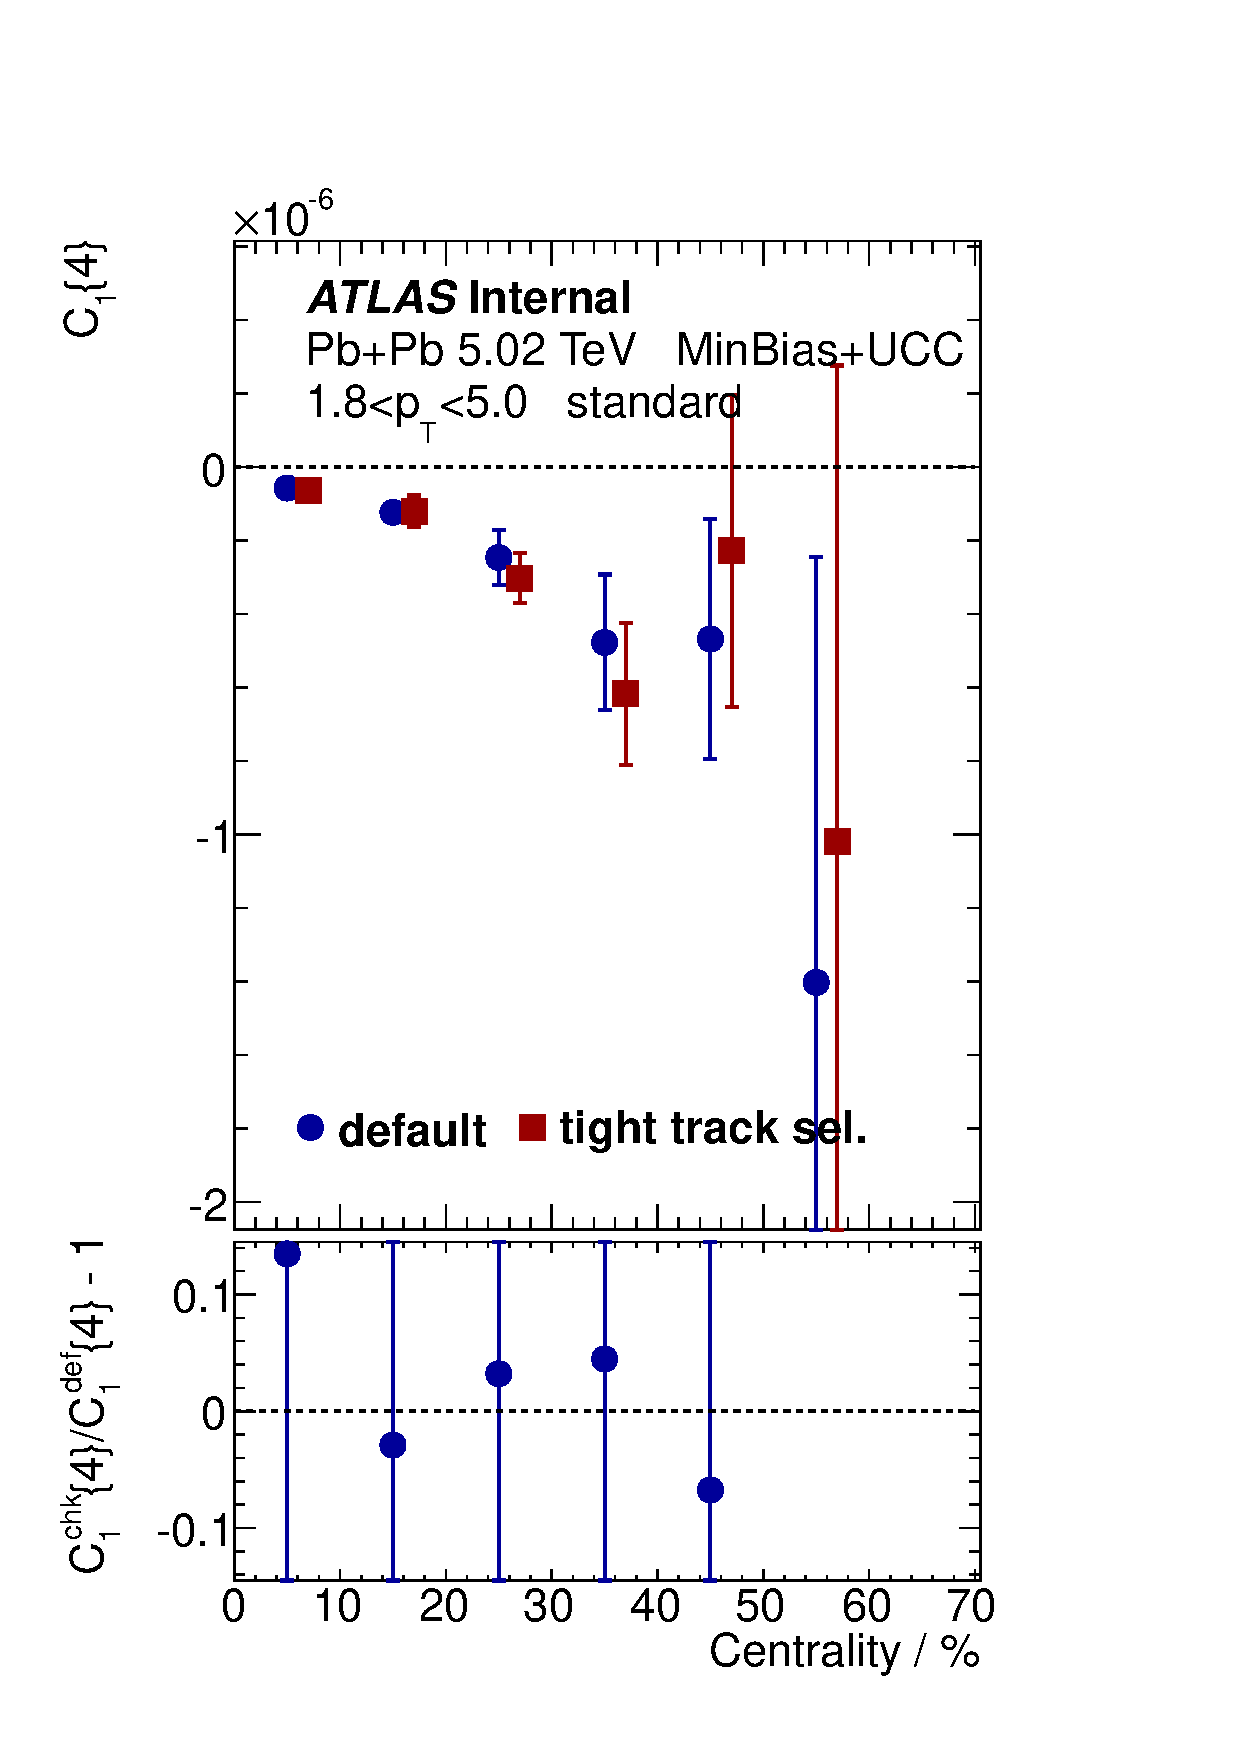
\includegraphics[width=.245\linewidth]{figs/sec_appendix/sys_PbPb502/PbPb502_sys3_1sub_Har1_Pt5.pdf}
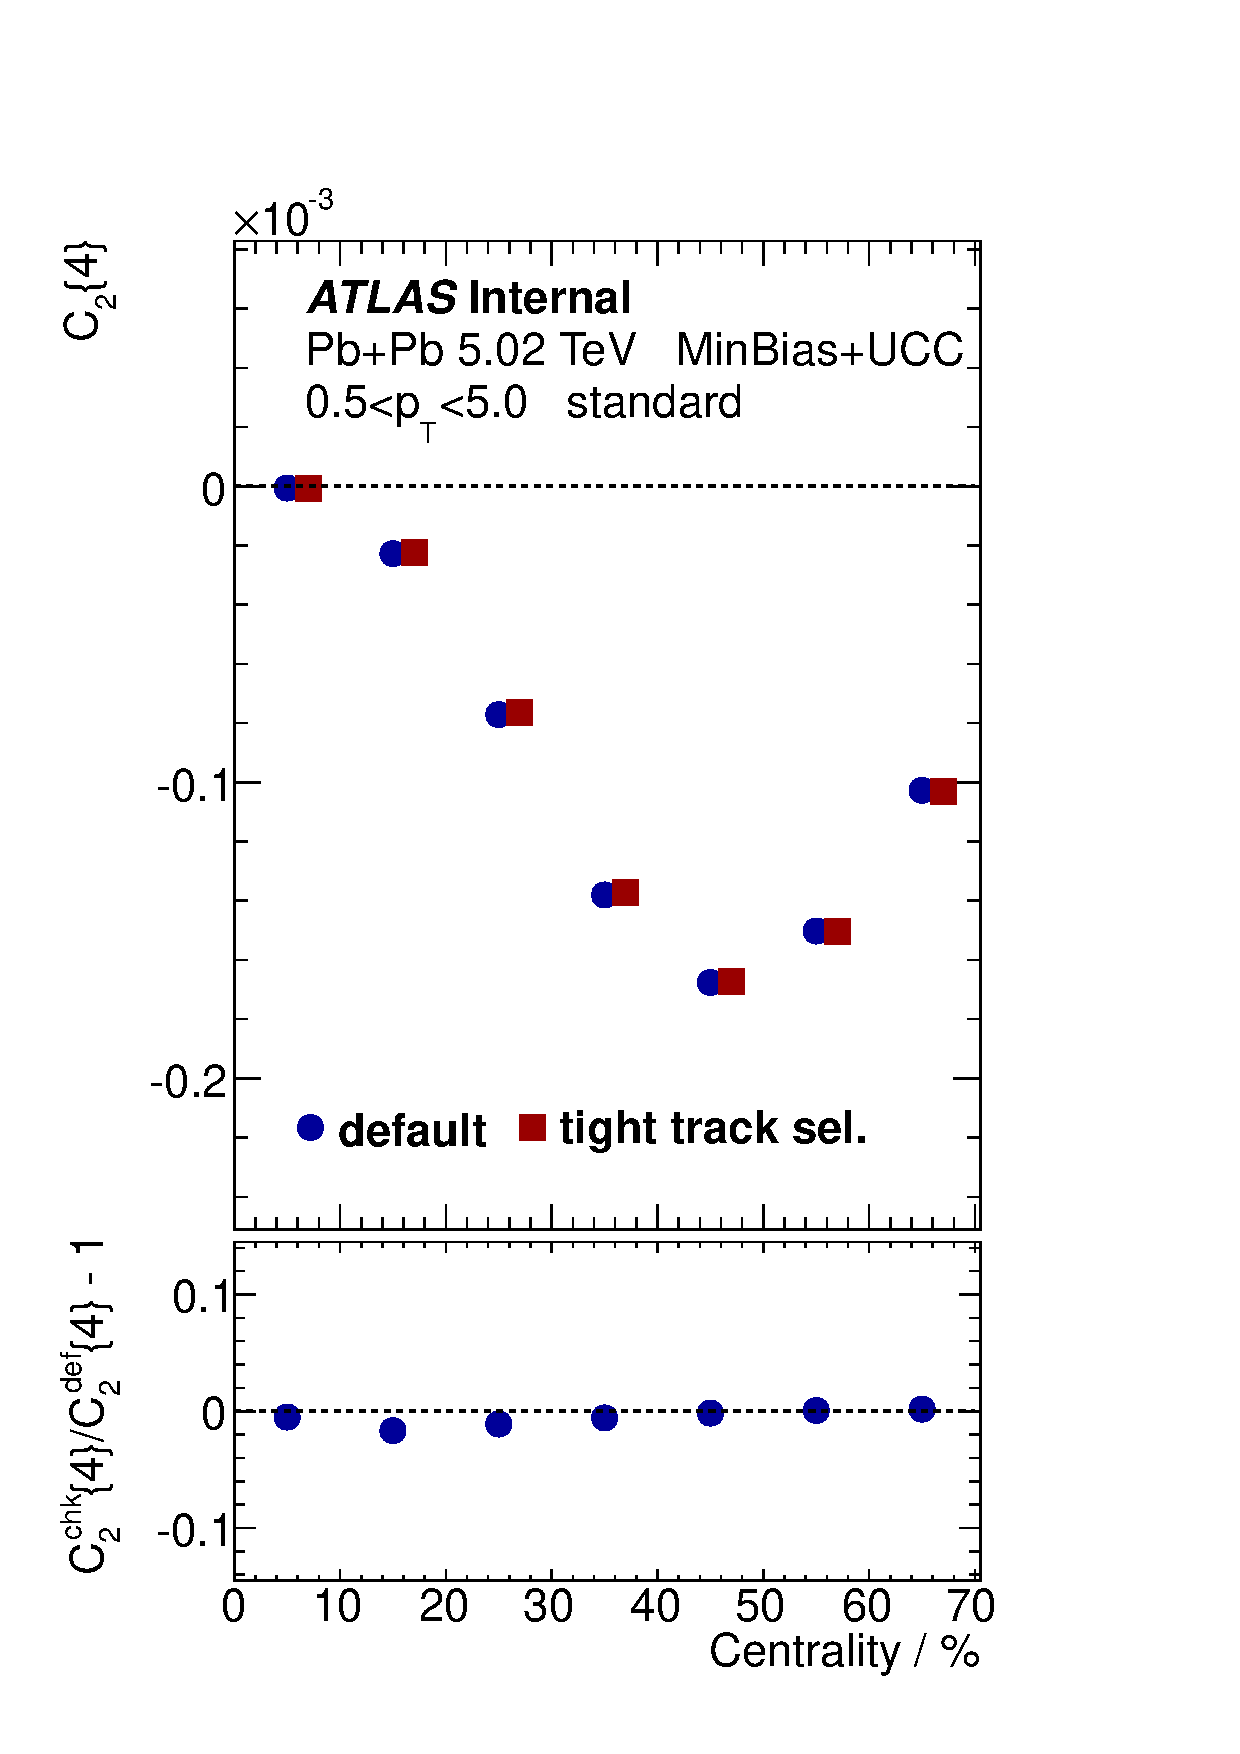
\includegraphics[width=.245\linewidth]{figs/sec_appendix/sys_PbPb502/PbPb502_sys3_1sub_Har2_Pt0.pdf}
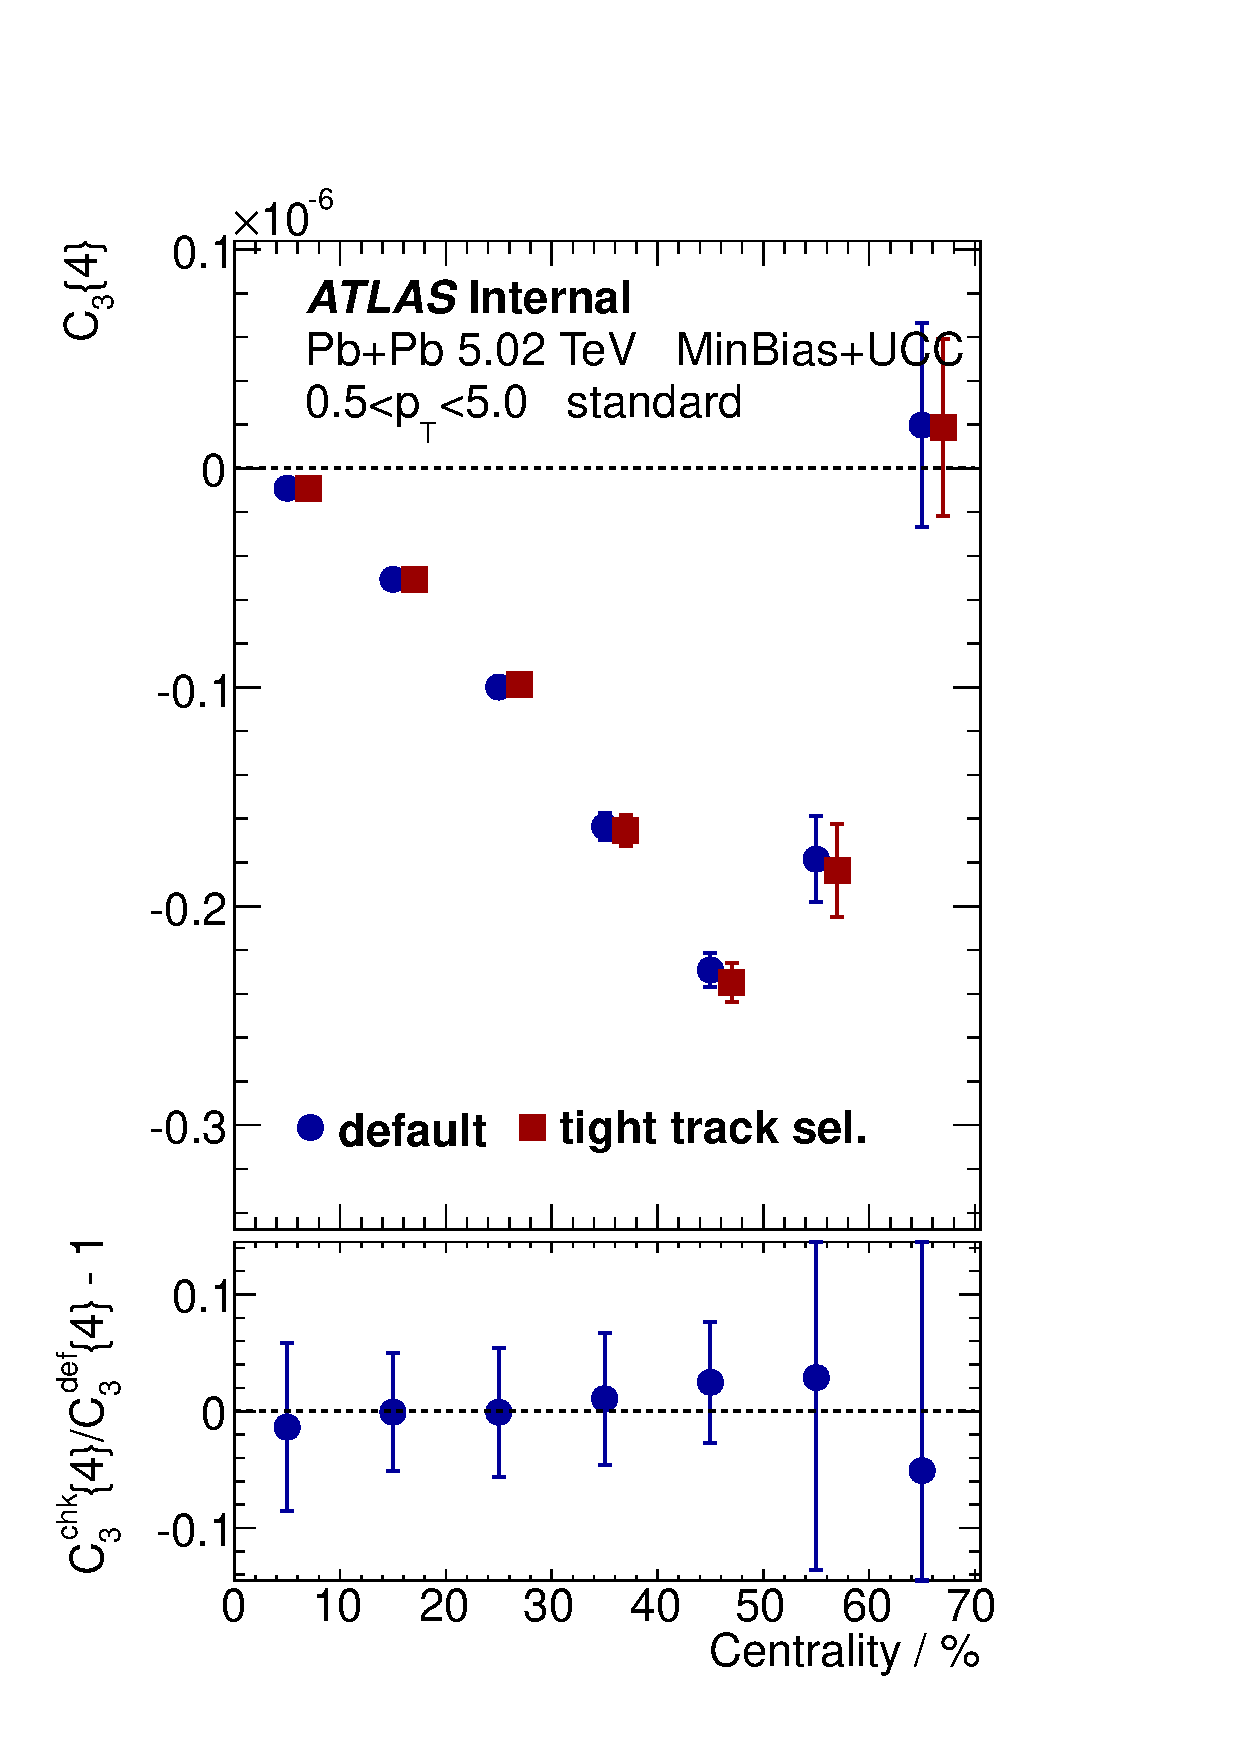
\includegraphics[width=.245\linewidth]{figs/sec_appendix/sys_PbPb502/PbPb502_sys3_1sub_Har3_Pt0.pdf}
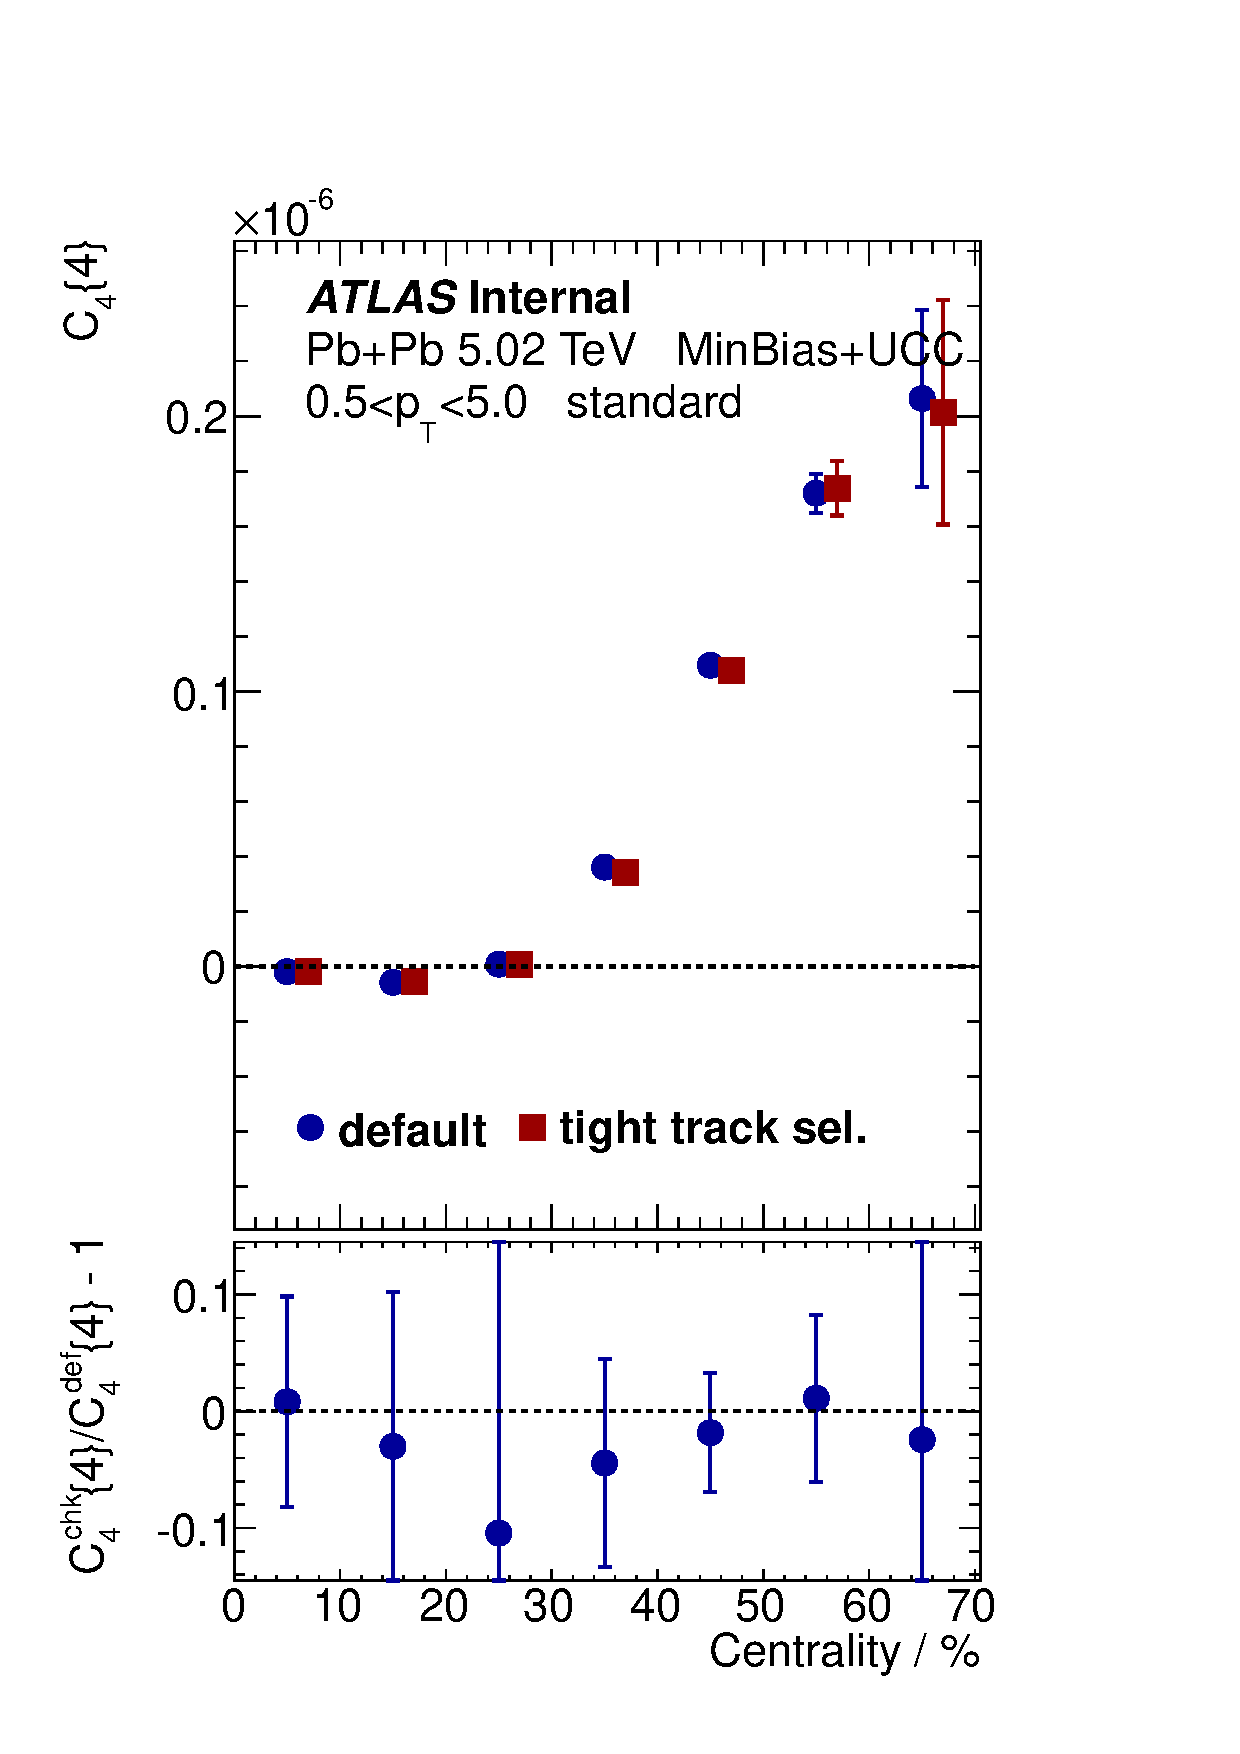
\includegraphics[width=.245\linewidth]{figs/sec_appendix/sys_PbPb502/PbPb502_sys3_1sub_Har4_Pt0.pdf}
\caption{Systematics of $c_n\{4\}$ from track selections: HI loose v.s. HI tight. Bottom panels are the relative uncertainties between the default and check.}
\label{fig:sys_trkSel}
\end{figure}



\subsection{Lower and higher tracking efficiency}
In this analysis, tracking efficiency is evaluated as a function of $p_\text{T}$, $\eta$ and centrality. Previous flow measurements have shown that $v_n$ strongly depends on $p_\text{T}$: it increases then decreases as $p_\text{T}$ increases. Meanwhile, differential flow measurements also shows that $v_n$ is weakly dependent of $\eta$. Due to these reasons, the $p_\text{T}$ weighting in tracking efficiency could introduce uncertainty to the results.

To evaluate the impact from uncertainty in the tracking efficiency, the following checks are performed:
\begin{itemize}
\item Default $\epsilon$: particles weighted by tracking efficiency;
\item Check 1 higher efficiency $\epsilon_+$: tracking efficiency in high $p_\text{T}$ is increased to its maximum within uncertainty; while tracking efficiency in low $p_\text{T}$ is decreased to its minimum within uncertainty;
\item Check 2 lower efficiency $\epsilon_-$: tracking efficiency in high $p_\text{T}$ is decreased to its minimum within uncertainty; while tracking efficiency in low $p_\text{T}$ is increased to its maximum within uncertainty;
\end{itemize}
where the two checks can be parameterized as:
\begin{equation}
\epsilon_\pm(p_\text{T}) \equiv \epsilon(p_\text{T}) \pm 0.06\frac{\epsilon(p_\text{T})-\epsilon(p_\text{T}^\text{low})}{\epsilon(p_\text{T}^\text{high})-\epsilon(p_\text{T}^\text{low})} \mp 0.03
\end{equation}
where $p_\text{T}^\text{low}$ is 0.5 GeV while $p_\text{T}^\text{high}$ is 5.0 GeV, which are the minimum and maximum $p_{T}$ ranges of this analysis.

\begin{figure}[H]
\centering
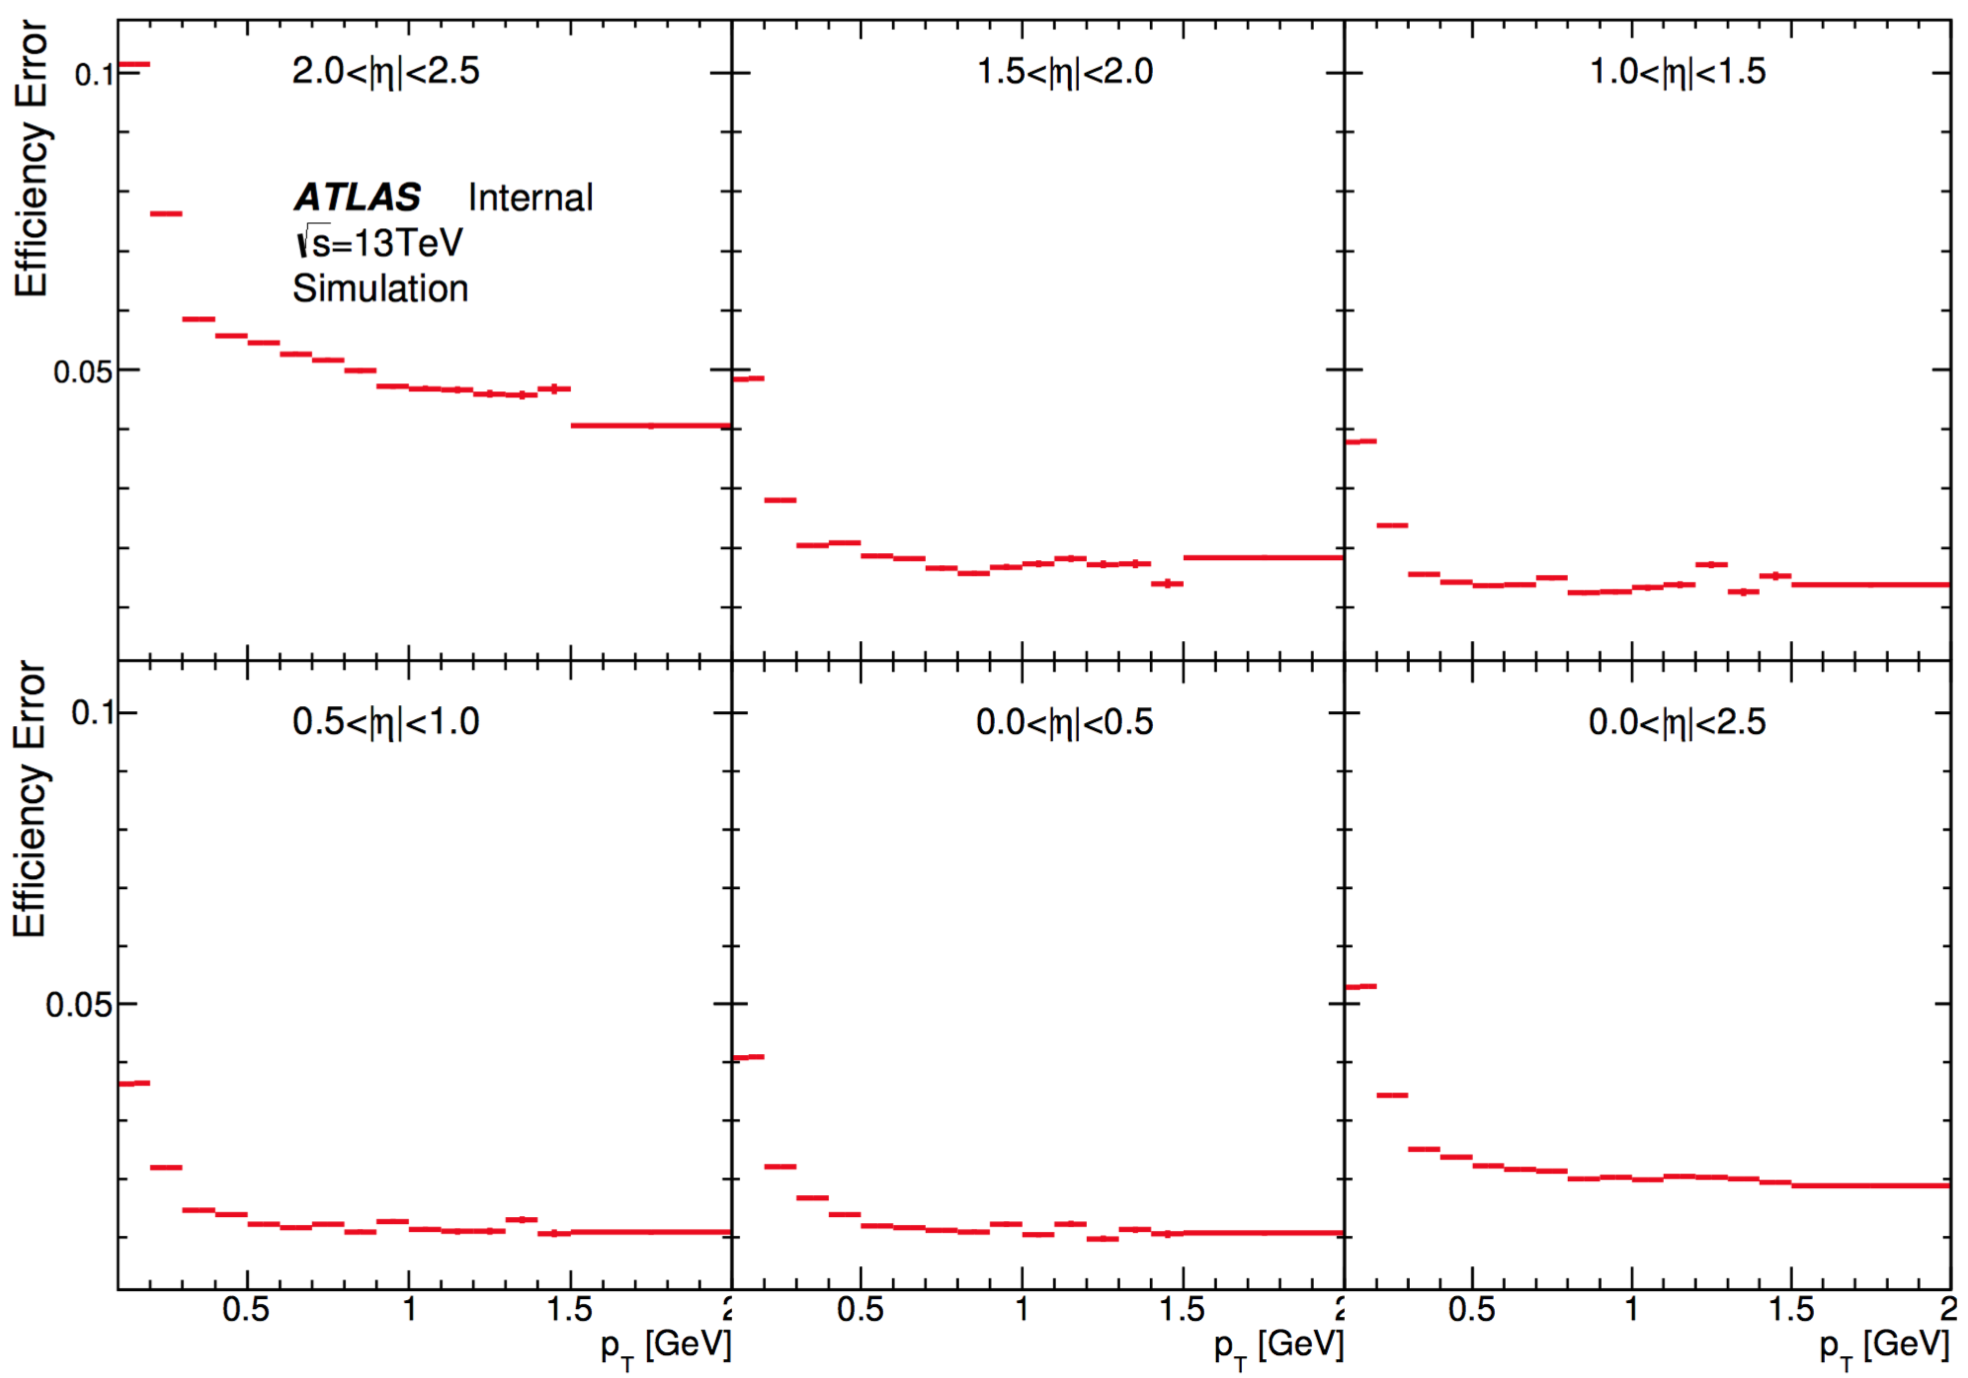
\includegraphics[width=.9\linewidth]{figs/sec_sys/sys_tracking_error.png}
\caption{The systematic uncertainties of the tracking efficiency plotted as a function of $p_\text{T}$ for several $|\eta|$ slices. These include the material uncertainties. These were obtained from the 13 TeV multiplicity analysis.~\cite{Morley:2011604}}
\label{fig:sys_tracking_error}
\end{figure}
Note that $0.03$ was selected as the variation of the tracking efficiency, which has been evaluated in the Minimum Bias multiplicity in 13 TeV $pp$ analysis~\cite{Morley:2011604}. The total uncertainty in tracking is shown in Fig.~\ref{fig:sys_tracking_error}, and the maximum variation for $p_\text{T}>0.5$ GeV is about $3\%$.

Fig.~\ref{fig:sys_trkEffLow} and fig.~\ref{fig:sys_trkEffHigh} show the comparison of $c_n\{4\}$ calculated using default tracking efficiency and lower/higher variations. For all the harmonics, the relative differences have opposite sign between lower and higher efficiency, as expected due to the $p_\text{T}$ dependence of flow. The largest relative differences come from low $p_\text{T}$ range, and decrease quickly as minimum $p_\text{T}$ cut increase. This check will be quoted as part of the combined systematics.
\begin{figure}[H]
\centering
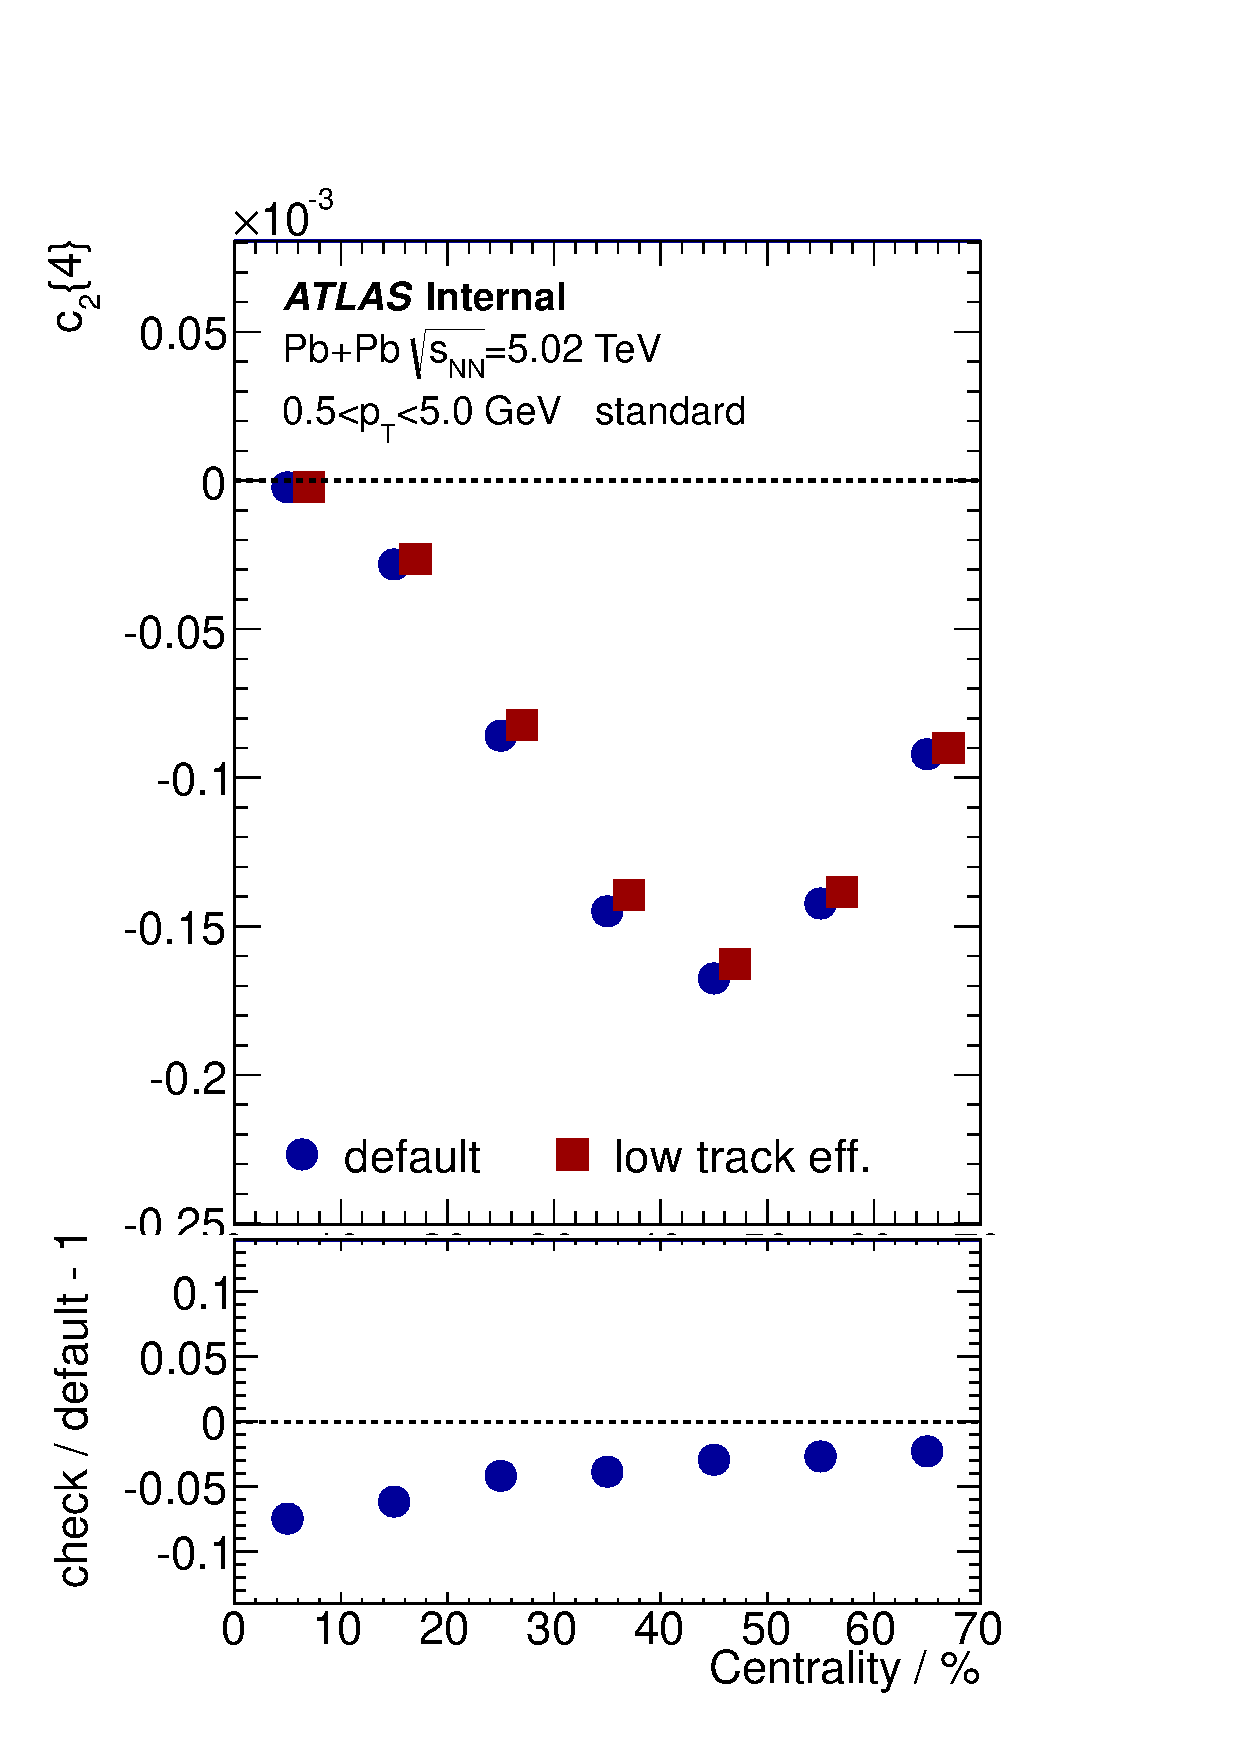
\includegraphics[width=.245\linewidth]{figs/sec_sys/summary/sys1_c4_1sub_Har2_Pt0.pdf}
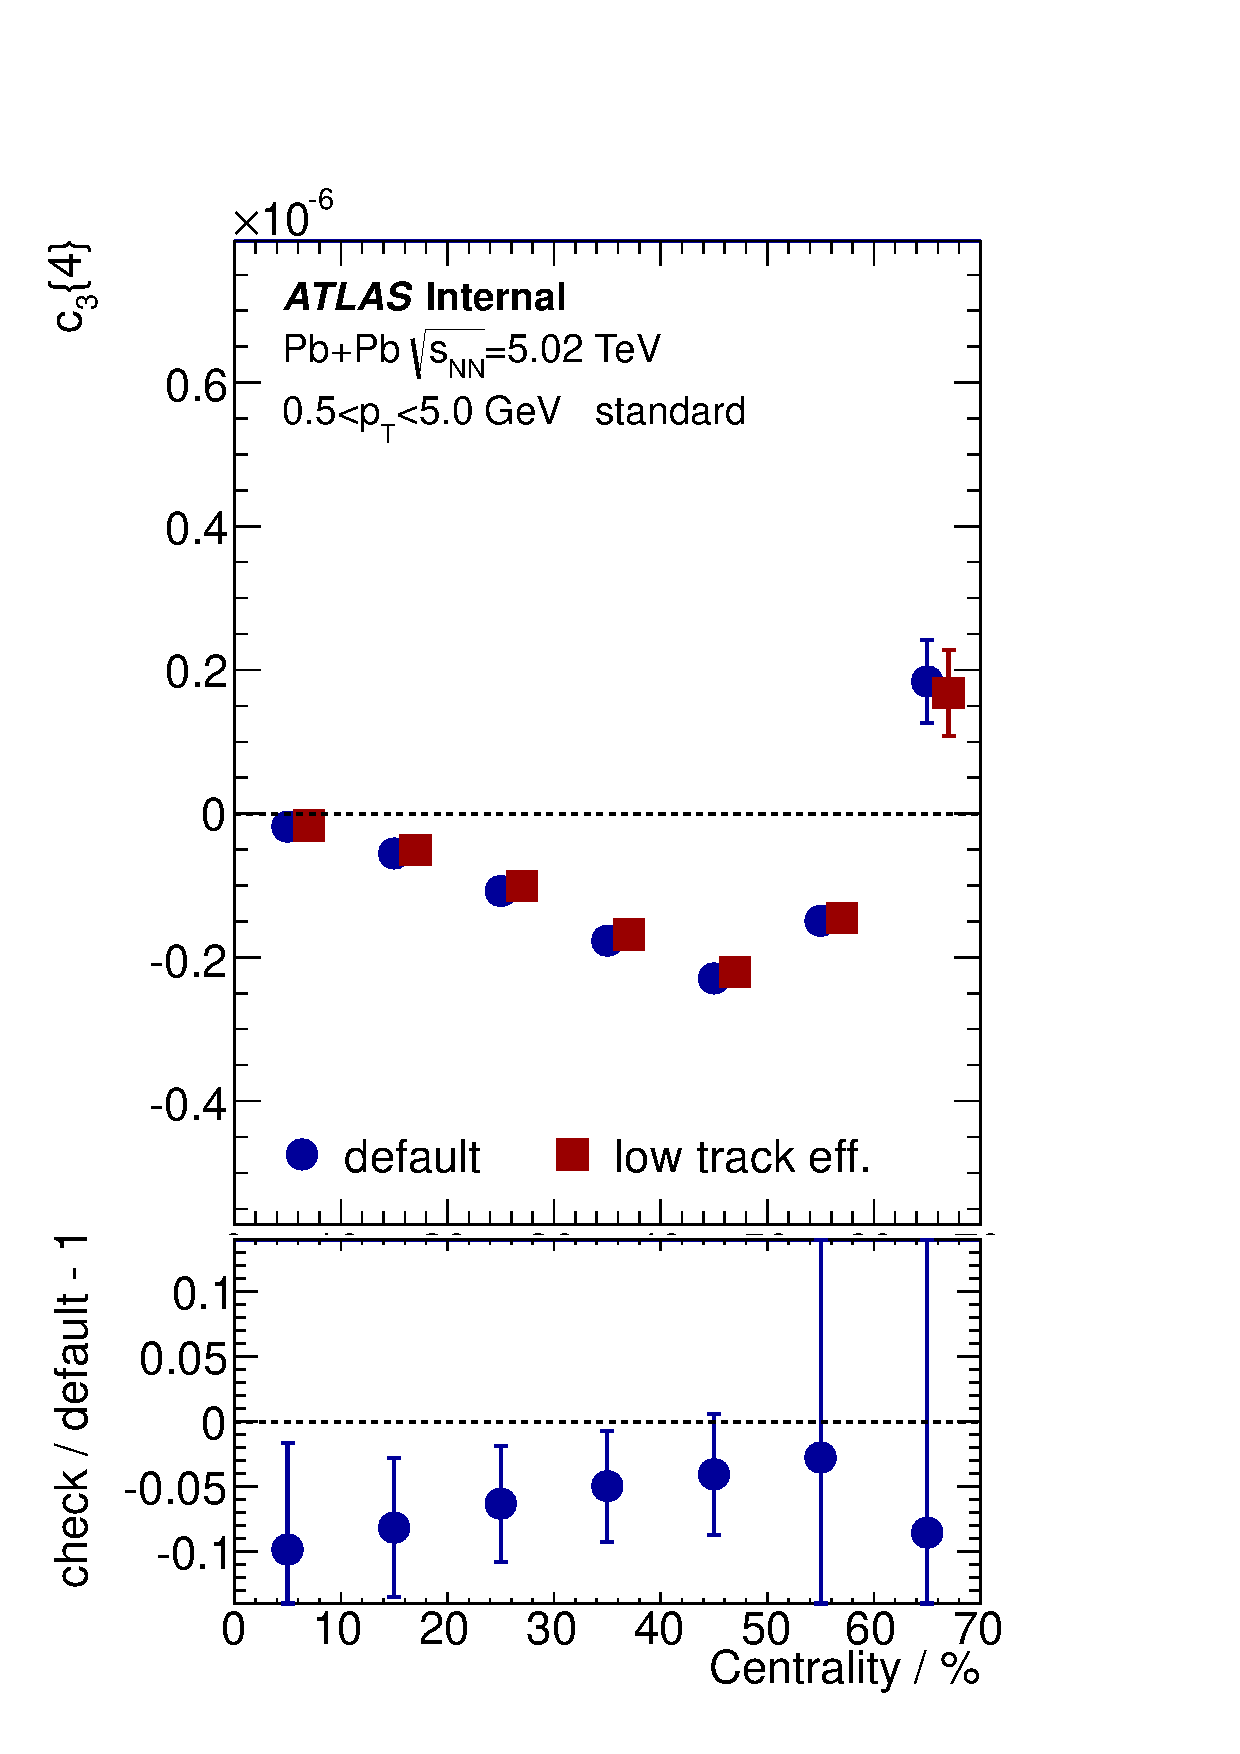
\includegraphics[width=.245\linewidth]{figs/sec_sys/summary/sys1_c4_1sub_Har3_Pt0.pdf}
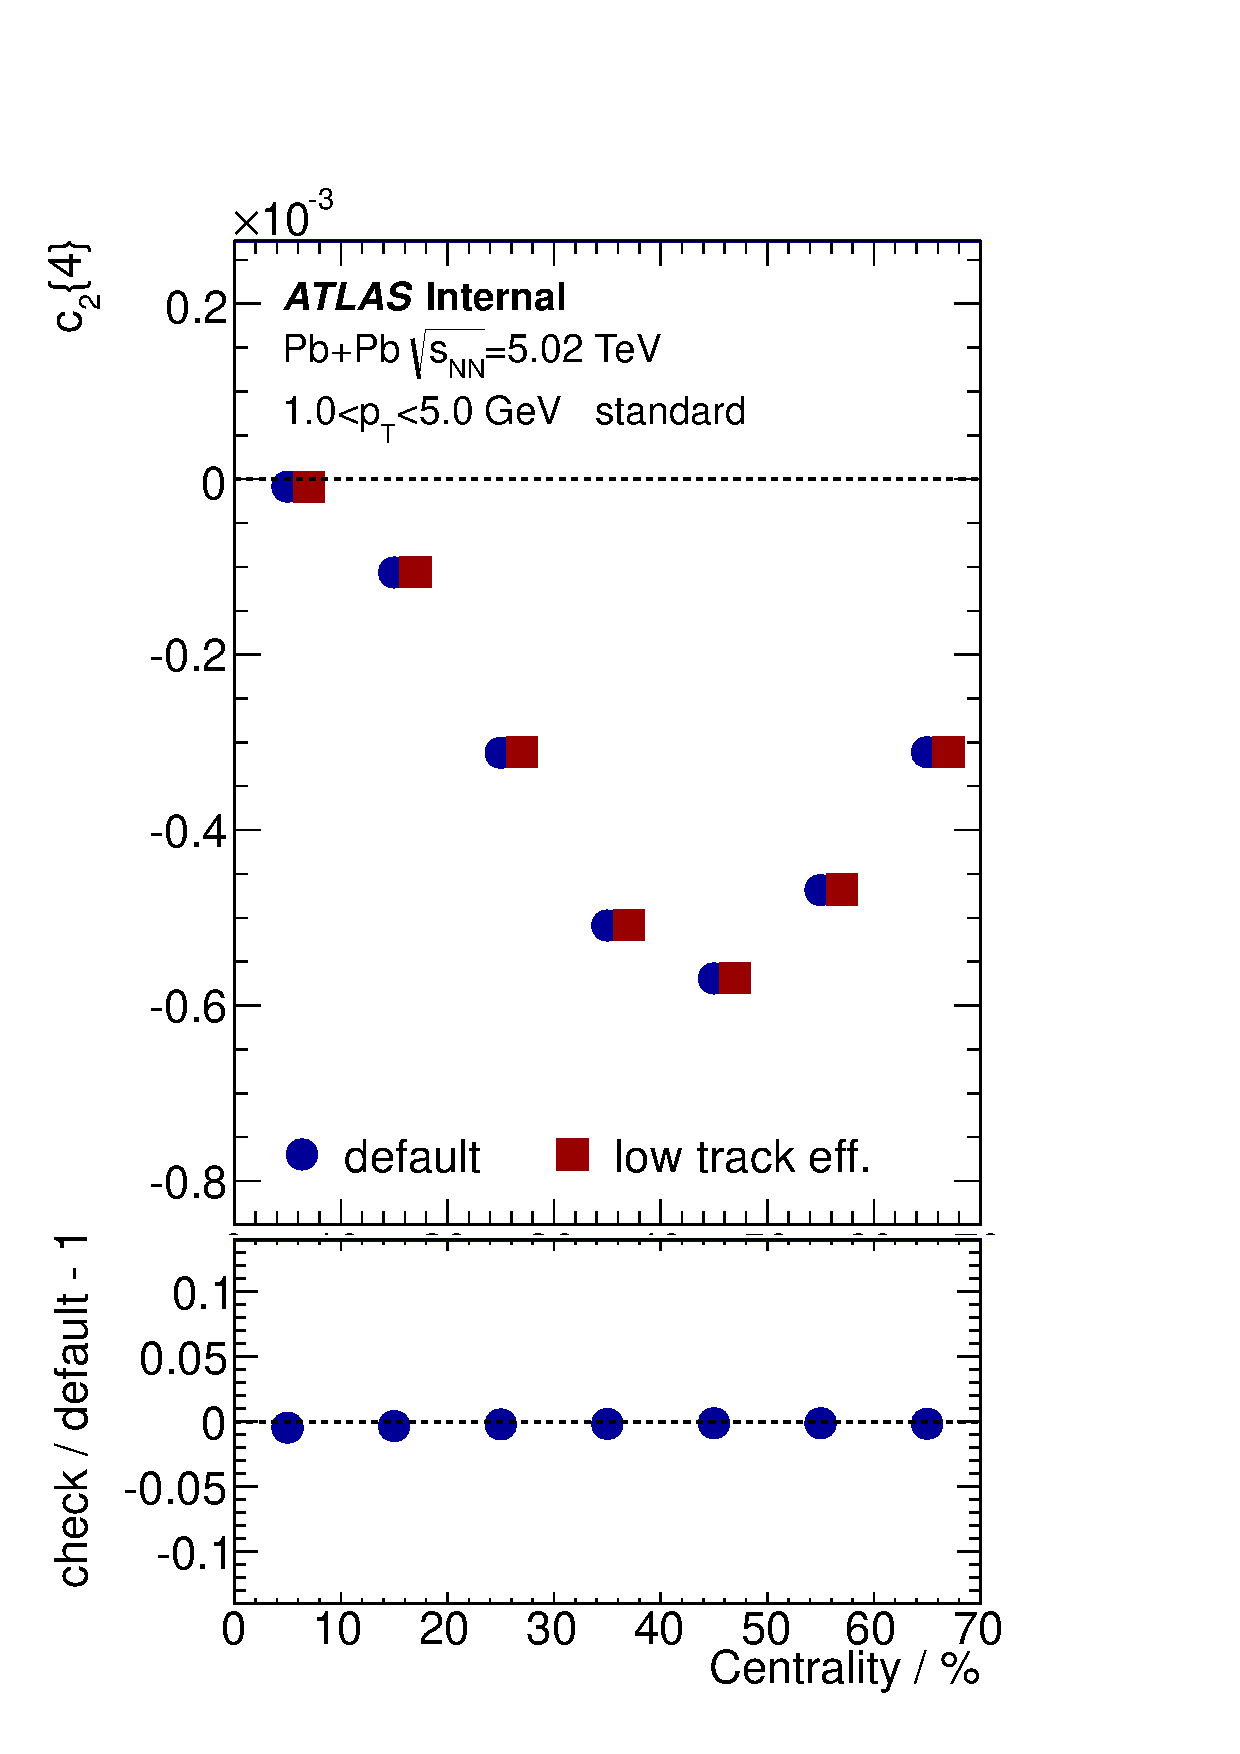
\includegraphics[width=.245\linewidth]{figs/sec_sys/summary/sys1_c4_1sub_Har2_Pt1.pdf}
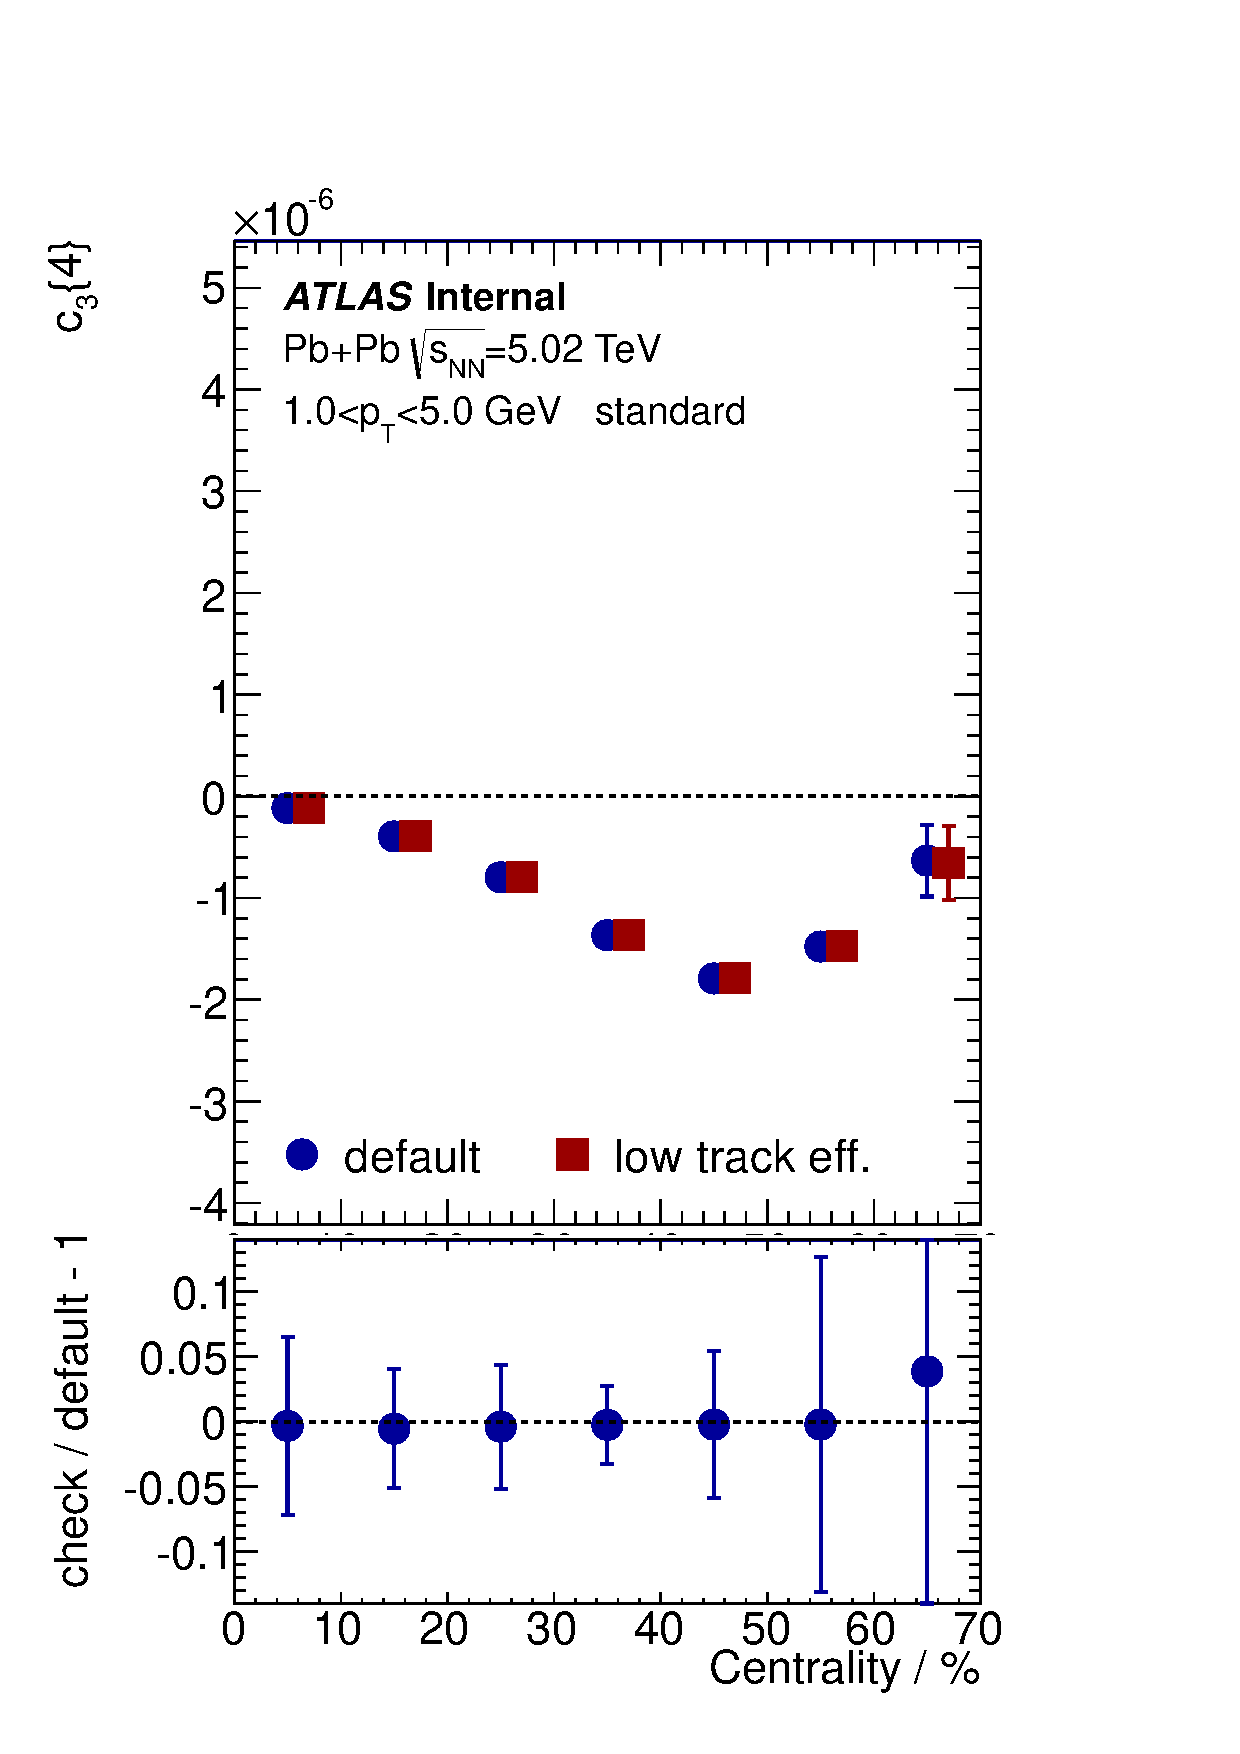
\includegraphics[width=.245\linewidth]{figs/sec_sys/summary/sys1_c4_1sub_Har3_Pt1.pdf}
\caption{Systematics of $c_n\{4\}$ from tracking efficiency: default v.s. lower efficiency. Bottom panels are the relative uncertainties between the default and check.}
\label{fig:sys_trkEffLow}
\end{figure}

\begin{figure}[H]
\centering
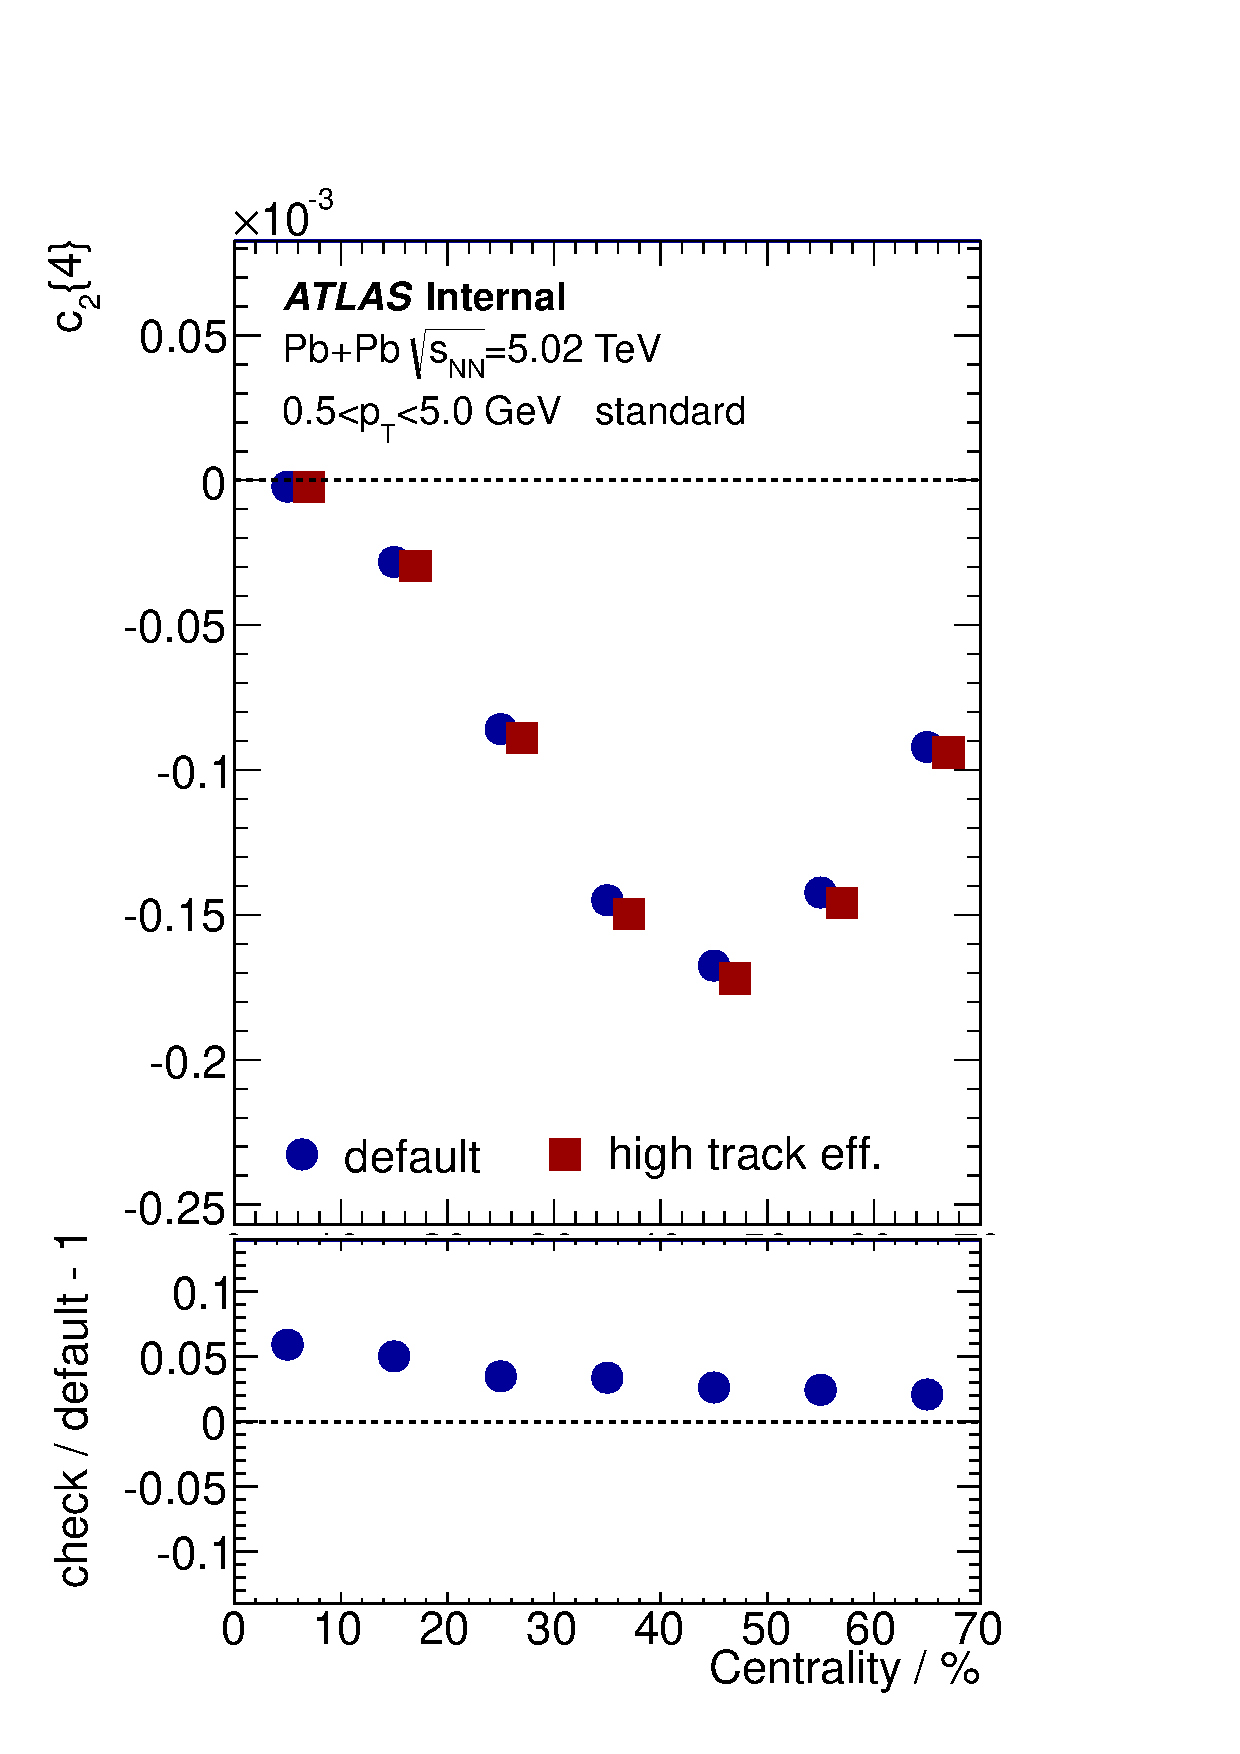
\includegraphics[width=.245\linewidth]{figs/sec_sys/summary/sys2_c4_1sub_Har2_Pt0.pdf}
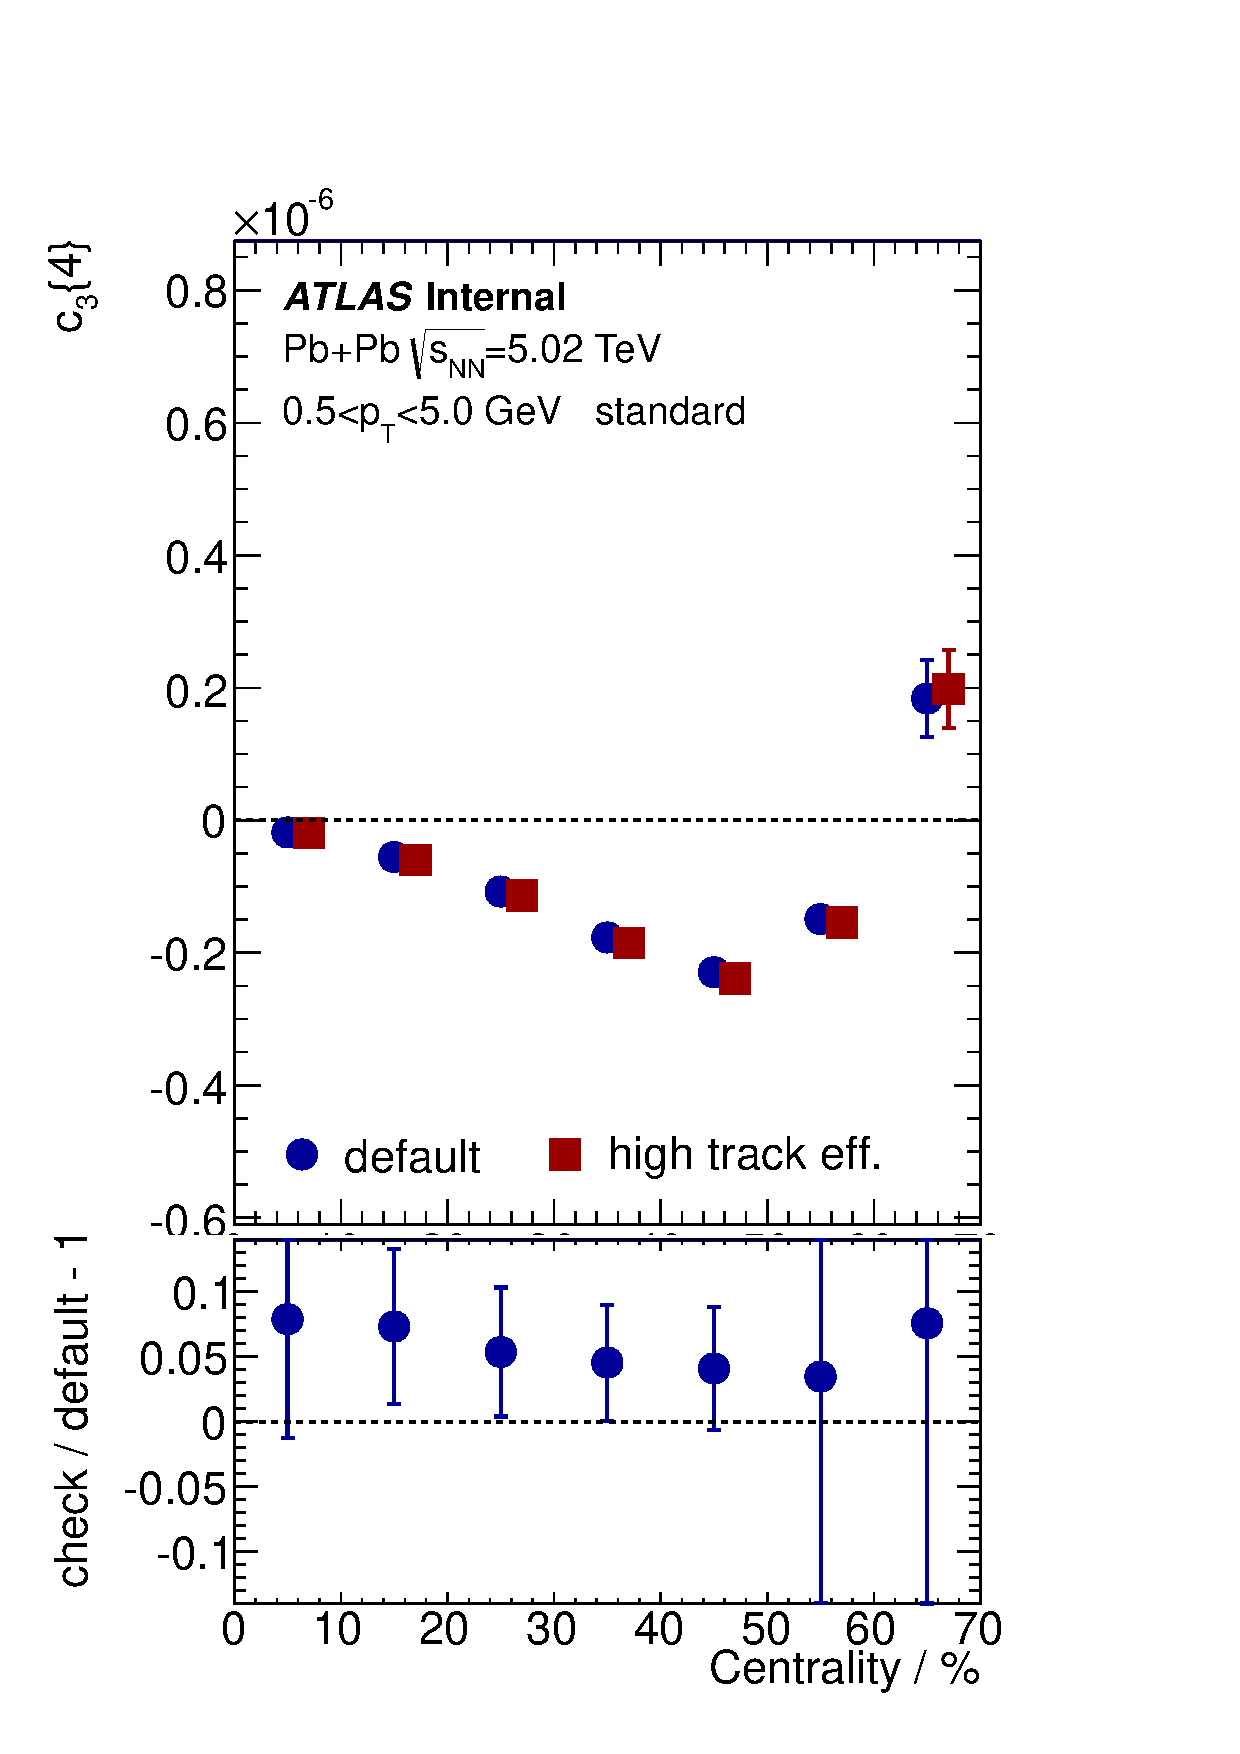
\includegraphics[width=.245\linewidth]{figs/sec_sys/summary/sys2_c4_1sub_Har3_Pt0.pdf}
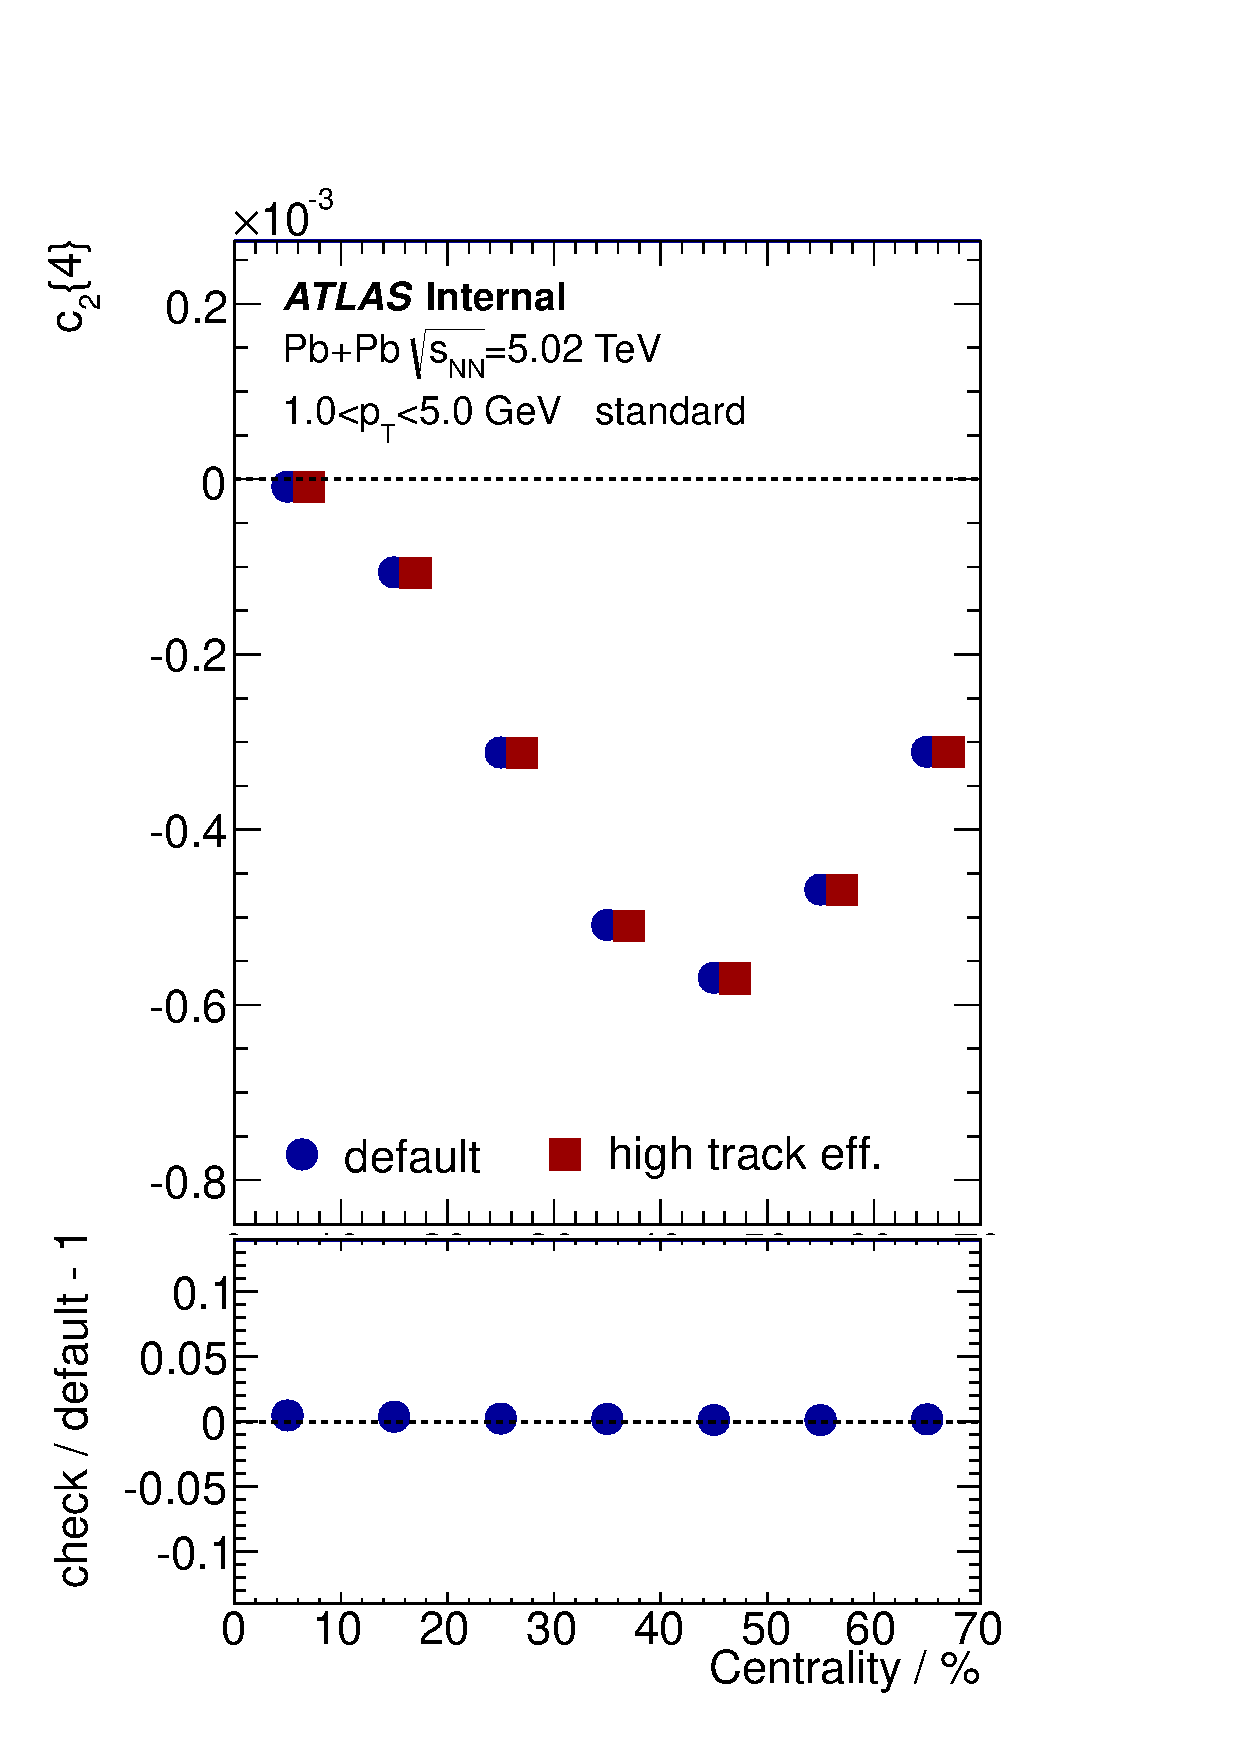
\includegraphics[width=.245\linewidth]{figs/sec_sys/summary/sys2_c4_1sub_Har2_Pt1.pdf}
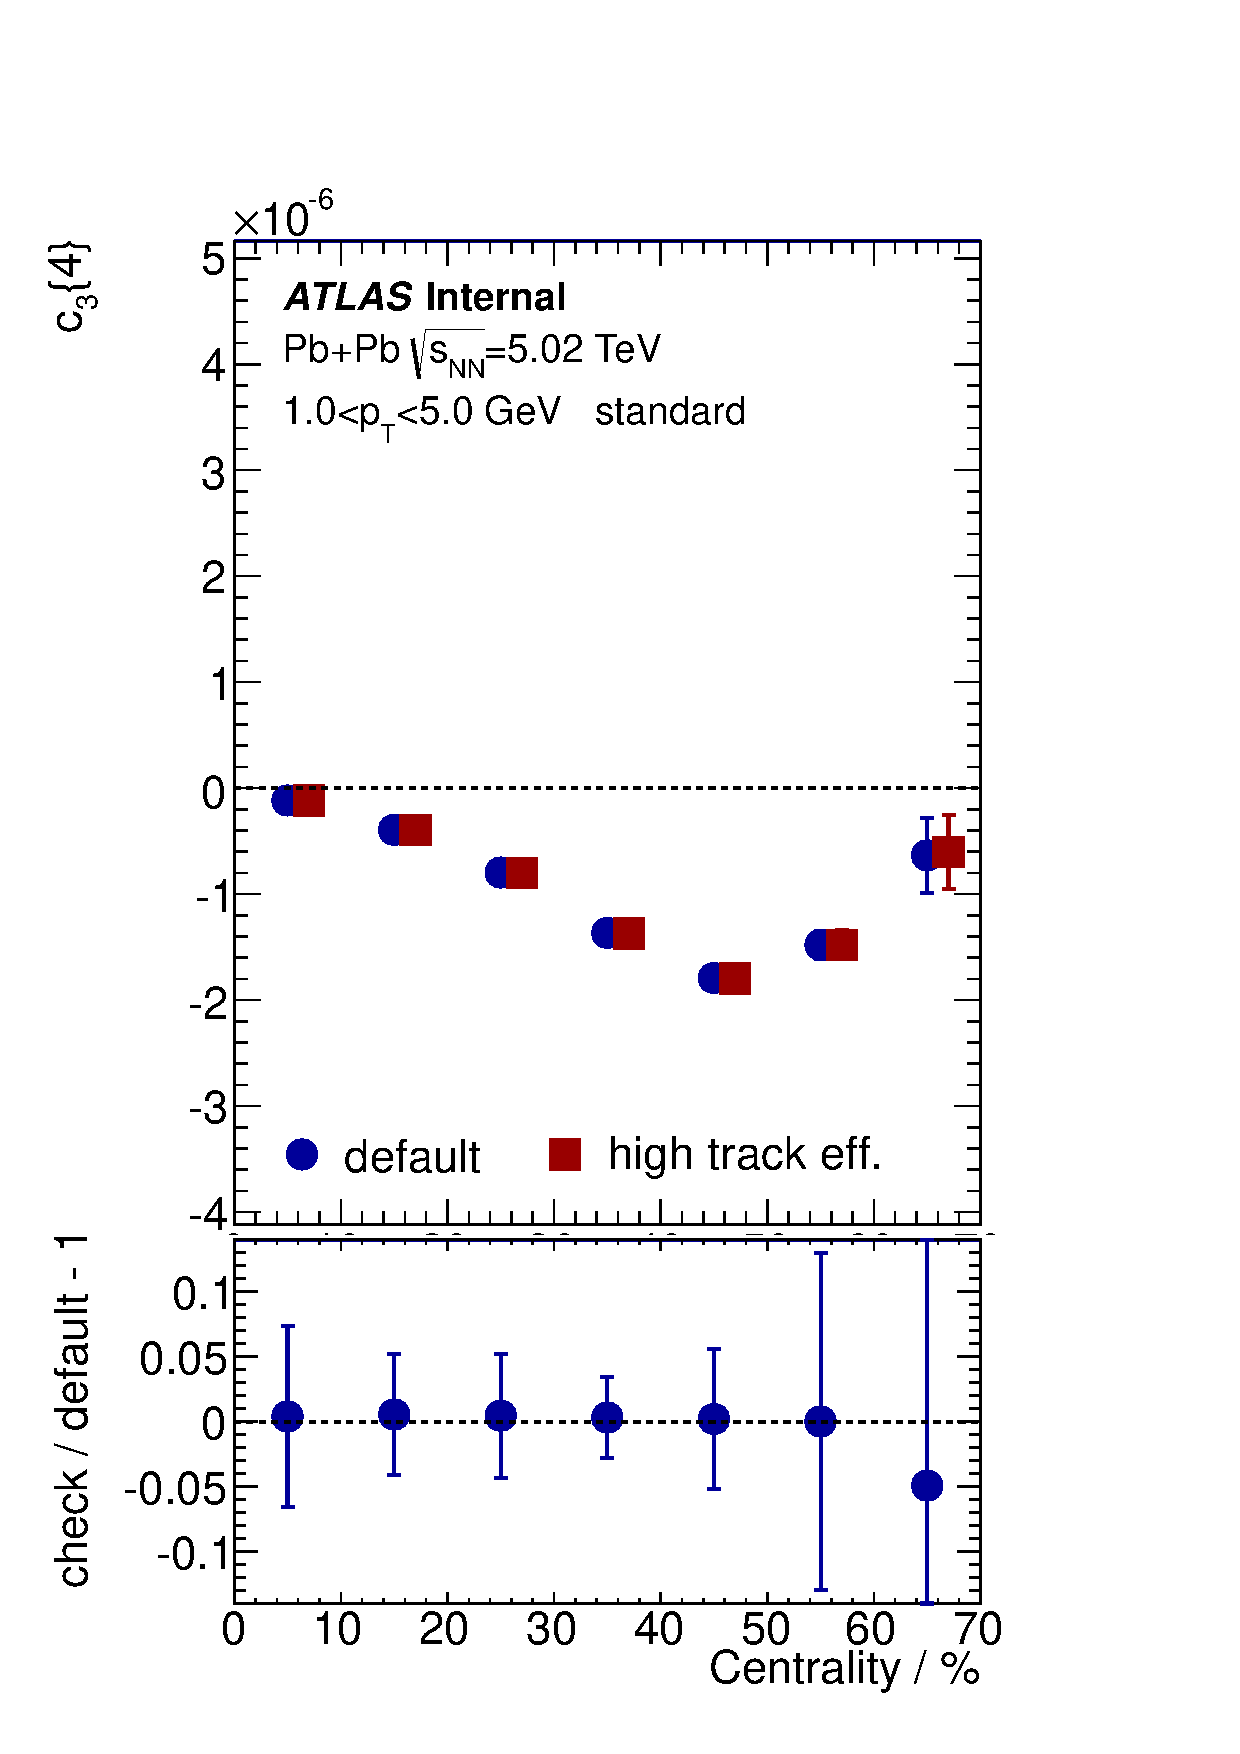
\includegraphics[width=.245\linewidth]{figs/sec_sys/summary/sys2_c4_1sub_Har3_Pt1.pdf}
\caption{Systematics of $c_n\{4\}$ from tracking efficiency: default v.s. higher efficiency. Bottom panels are the relative uncertainties between the default and check.}
\label{fig:sys_trkEffHigh}
\end{figure}



\subsection{Pileup rejection}
During the 2015 Pb+Pb data taking, the mean value of $\mu$ is around 0.001, which means the fraction of pileup events is very low compared with $pp$ or $p+$Pb samples. Furthermore, in this analysis all the tracks used to calculate cumulants are from the primary vertex. In principle, in pile-up events, tracks from pile-up vertex should not contribute to the measurement. However, in the track and vertex reconstruction, when a pile-up vertex is too close to the primary vertex, two vertices might be merged. Since the particles from two different vertices are totally uncorrelated, including these events with merged vertex will reduce the signal of flow signal.

In order to check the impact from pileup events, a variation of pileup cleaning is performed:
\begin{itemize}
\item Default: official HI pileup rejection tool, based on FCal $E_T$ and ZDC;
\item Check: alternative pileup rejection method, based on FCal $E_T$ and tracks $N_{ch}$;
\end{itemize}

Fig.~\ref{fig:sys_pu_eg} illustrates the differences between the two pileup cleaning methods: official (left) and alternative (right). The left panel shows the correlation between FCal sum $E_T$ and calibrated number of neutrons in the ZDC. The main band (light blue circle) is dominated by the events with a single primary vertex and the "grass" above the main band (light red circle) are mainly from pileup events. This is because both the sum $E_T$ and number of neutrons in a pileup event are larger than the corresponding single event. In order to clean up the pileup events, a significance cut (indicated by the red curve) was applied to reject the top $0.1\%$ events at each FCal sum $E_T$ slice. From this correlation map, it is obvious that the pileup events and single events are disentangled at very high FCal sum $E_T$, meaning that almost all the pileup events are rejected with the official pileup tool. As a comparison, the right panel shows the correlation between FCal sum $E_T$ and the number of tracking efficiency corrected reconstructed tracks $N_{ch}$. Similar as the left panel, the "grass" under the main band are from the pileup events. However, since FCal sum $E_T$ and $N_{ch}$ are correlated, the overlap region between the pileup events and single events is much larger than the previous case, where the $N_\text{neutron}$ and FCal sum $E_T$ are anti-correlated. This means the performance of this alternative pileup rejection method is much worse than the official, which provides sufficient variations as a cross-check.
\begin{figure}[H]
\centering
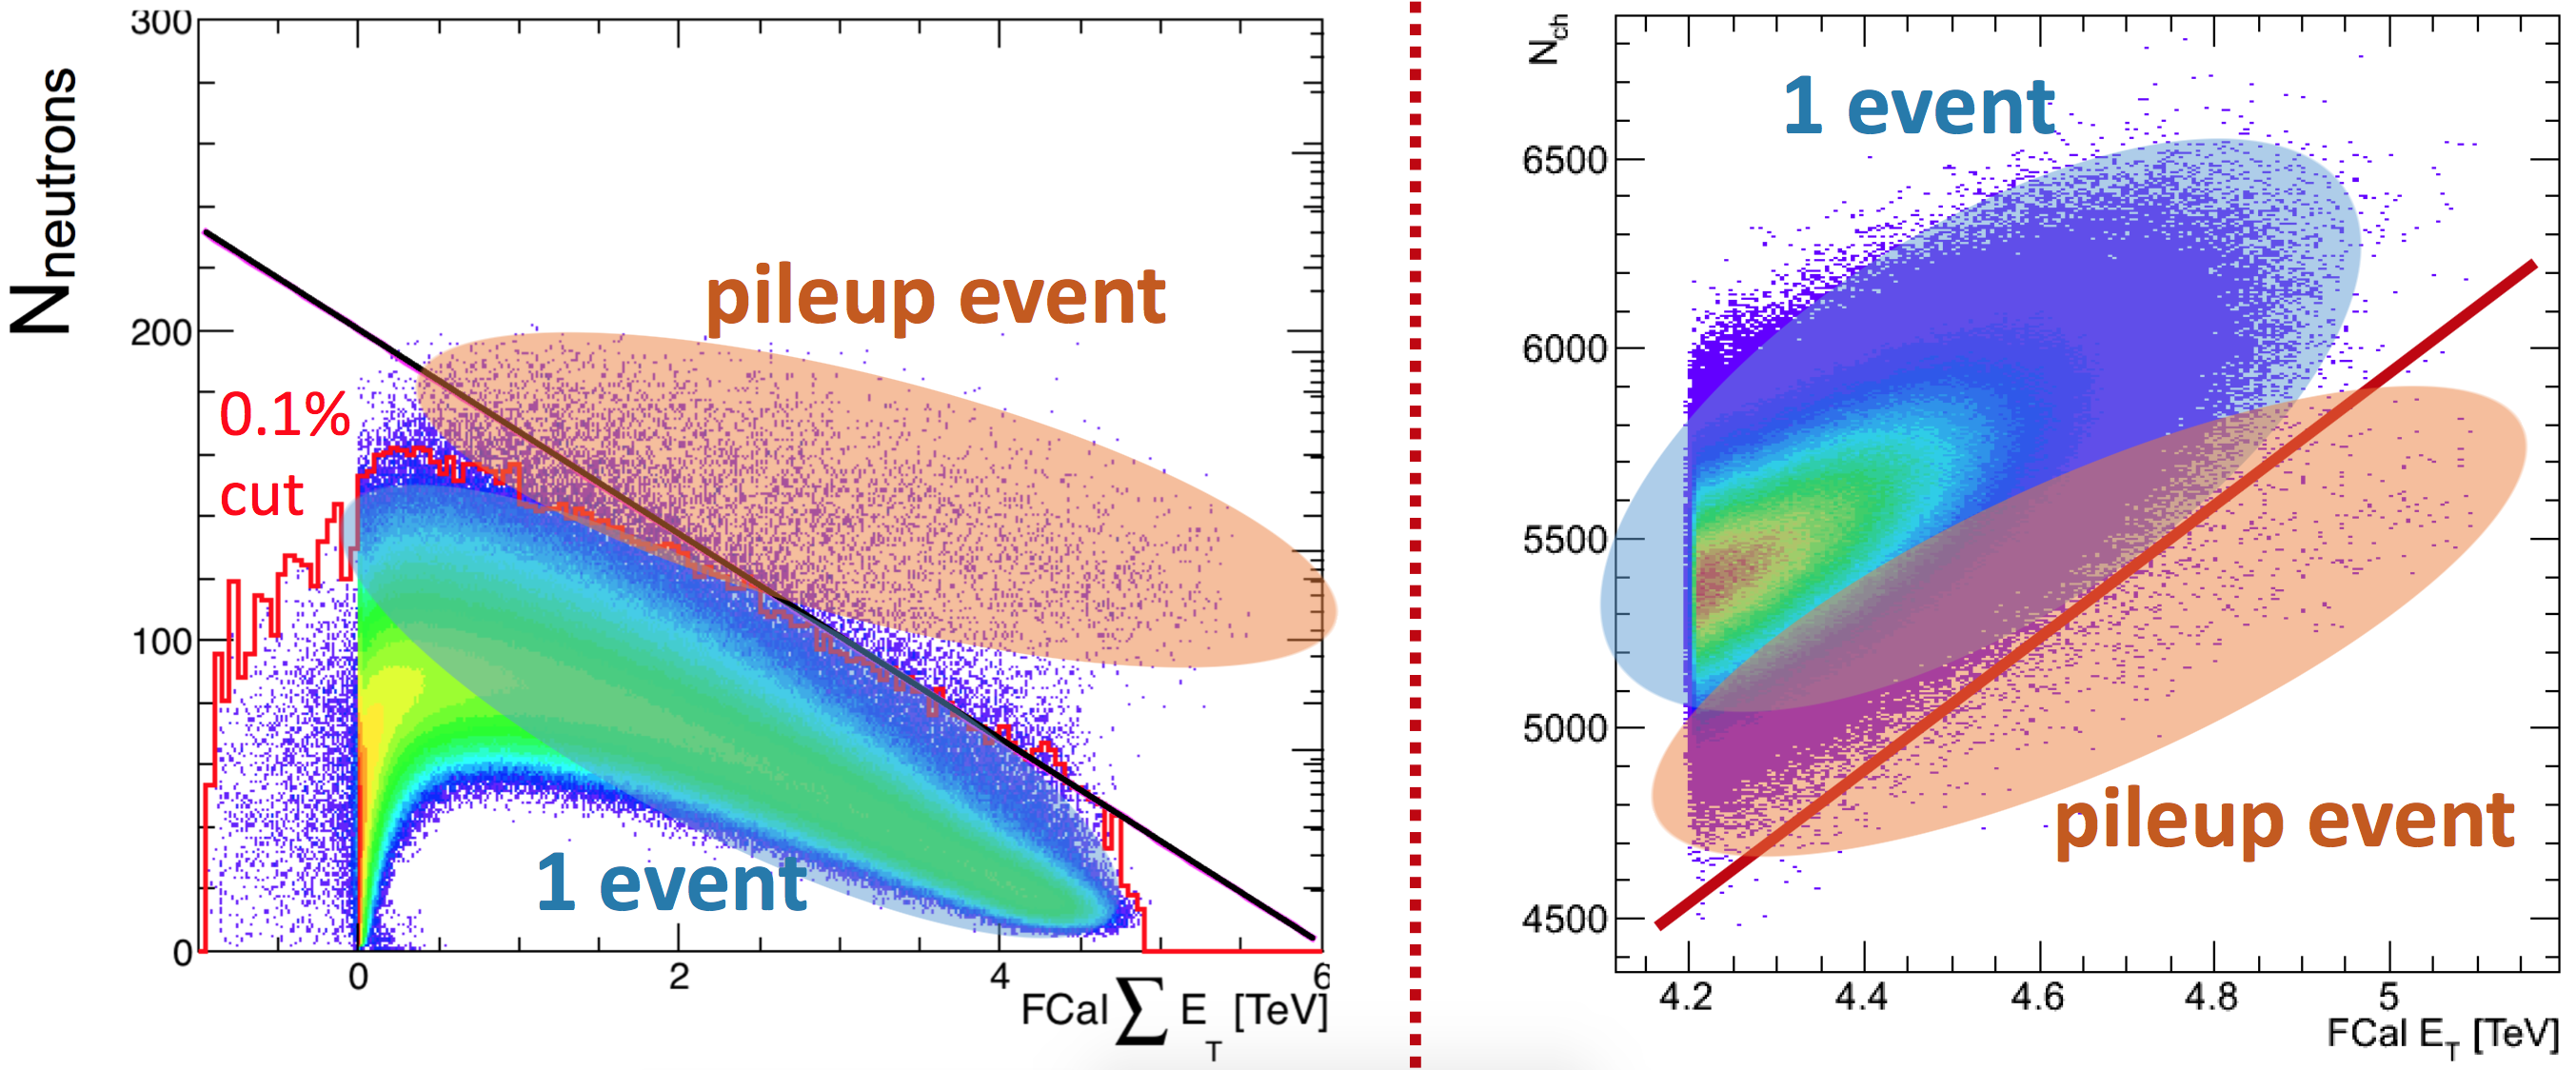
\includegraphics[width=.9\linewidth]{figs/sec_sys/pu_eg.png}
\caption{An illustration of two pileup rejection methods: official HI pileup tool (left) and private pileup rejection (right).}
\label{fig:sys_pu_eg}
\end{figure}

The fraction of pileup events in peripheral is minimal and it increases fast with FCal $E_{T}$, so only comparisons in UCC events are shown. But note that this systematic check is also performed for the whole centrality range. It is worth mentioning that this check overestimates the pileup impact since the fraction of residual pileup events are large using the alternative rejection. Another way to estimate the impact from pileup would be by adjusting the significance cut of $N_\text{neutrons}$, and check the trend of $c_n\{4\}$ as a function of various ZDC energy cut. To be conservative, we are quoting the difference between the two methods as the upper bond of the systematics for pileup effects.

The comparison of $c_n\{4\}$ calculated with and without pileup rejection is shown in Fig.~\ref{fig:sys_pu}, as a function of FCal $E_{T}$ in ultra-central collisions. For all the harmonics, the relative differences are within $10\%$ and within statistical uncertainties. It is quoted as part of the systematics.

\begin{figure}[H]
\centering
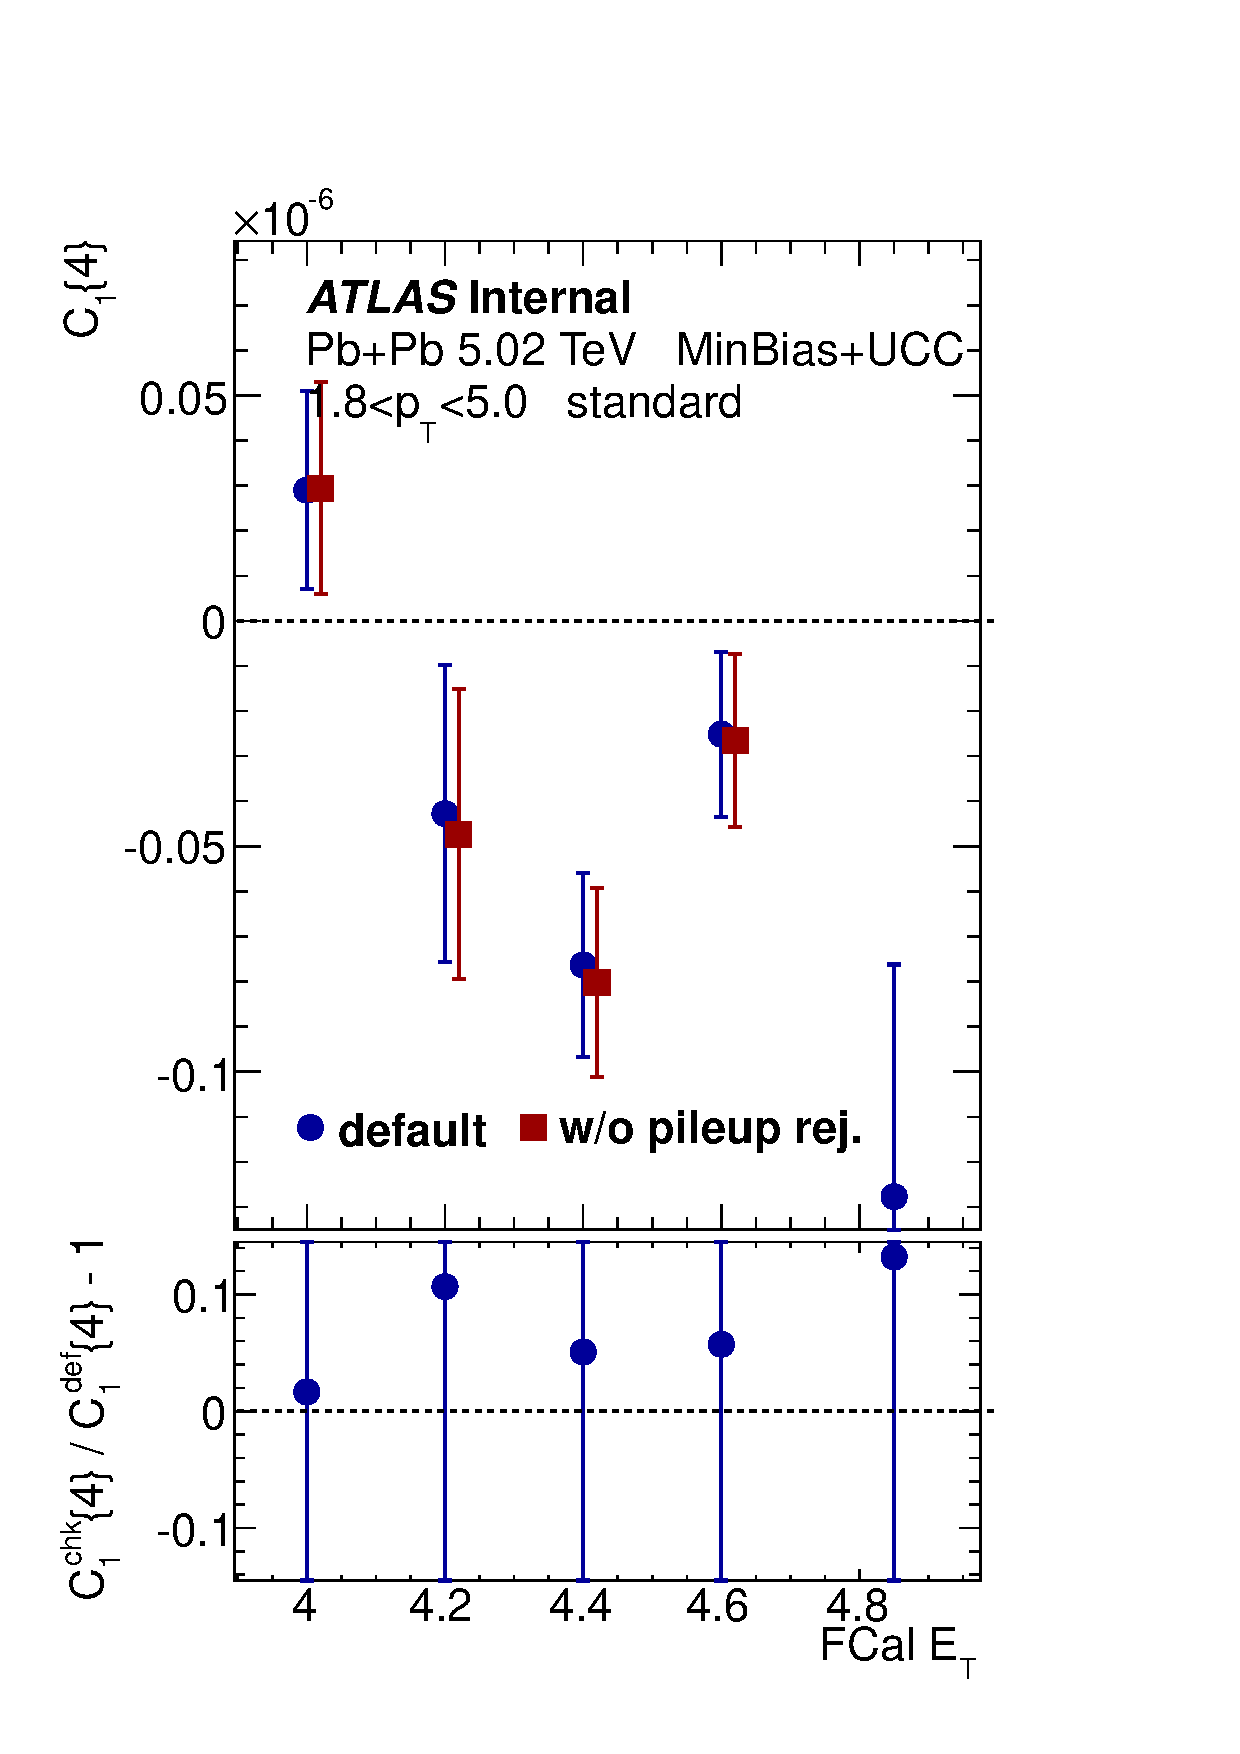
\includegraphics[width=.245\linewidth]{figs/sec_appendix/sys_PbPb502_UCC/PbPb502_sys4_1sub_Har1_Pt5.pdf}
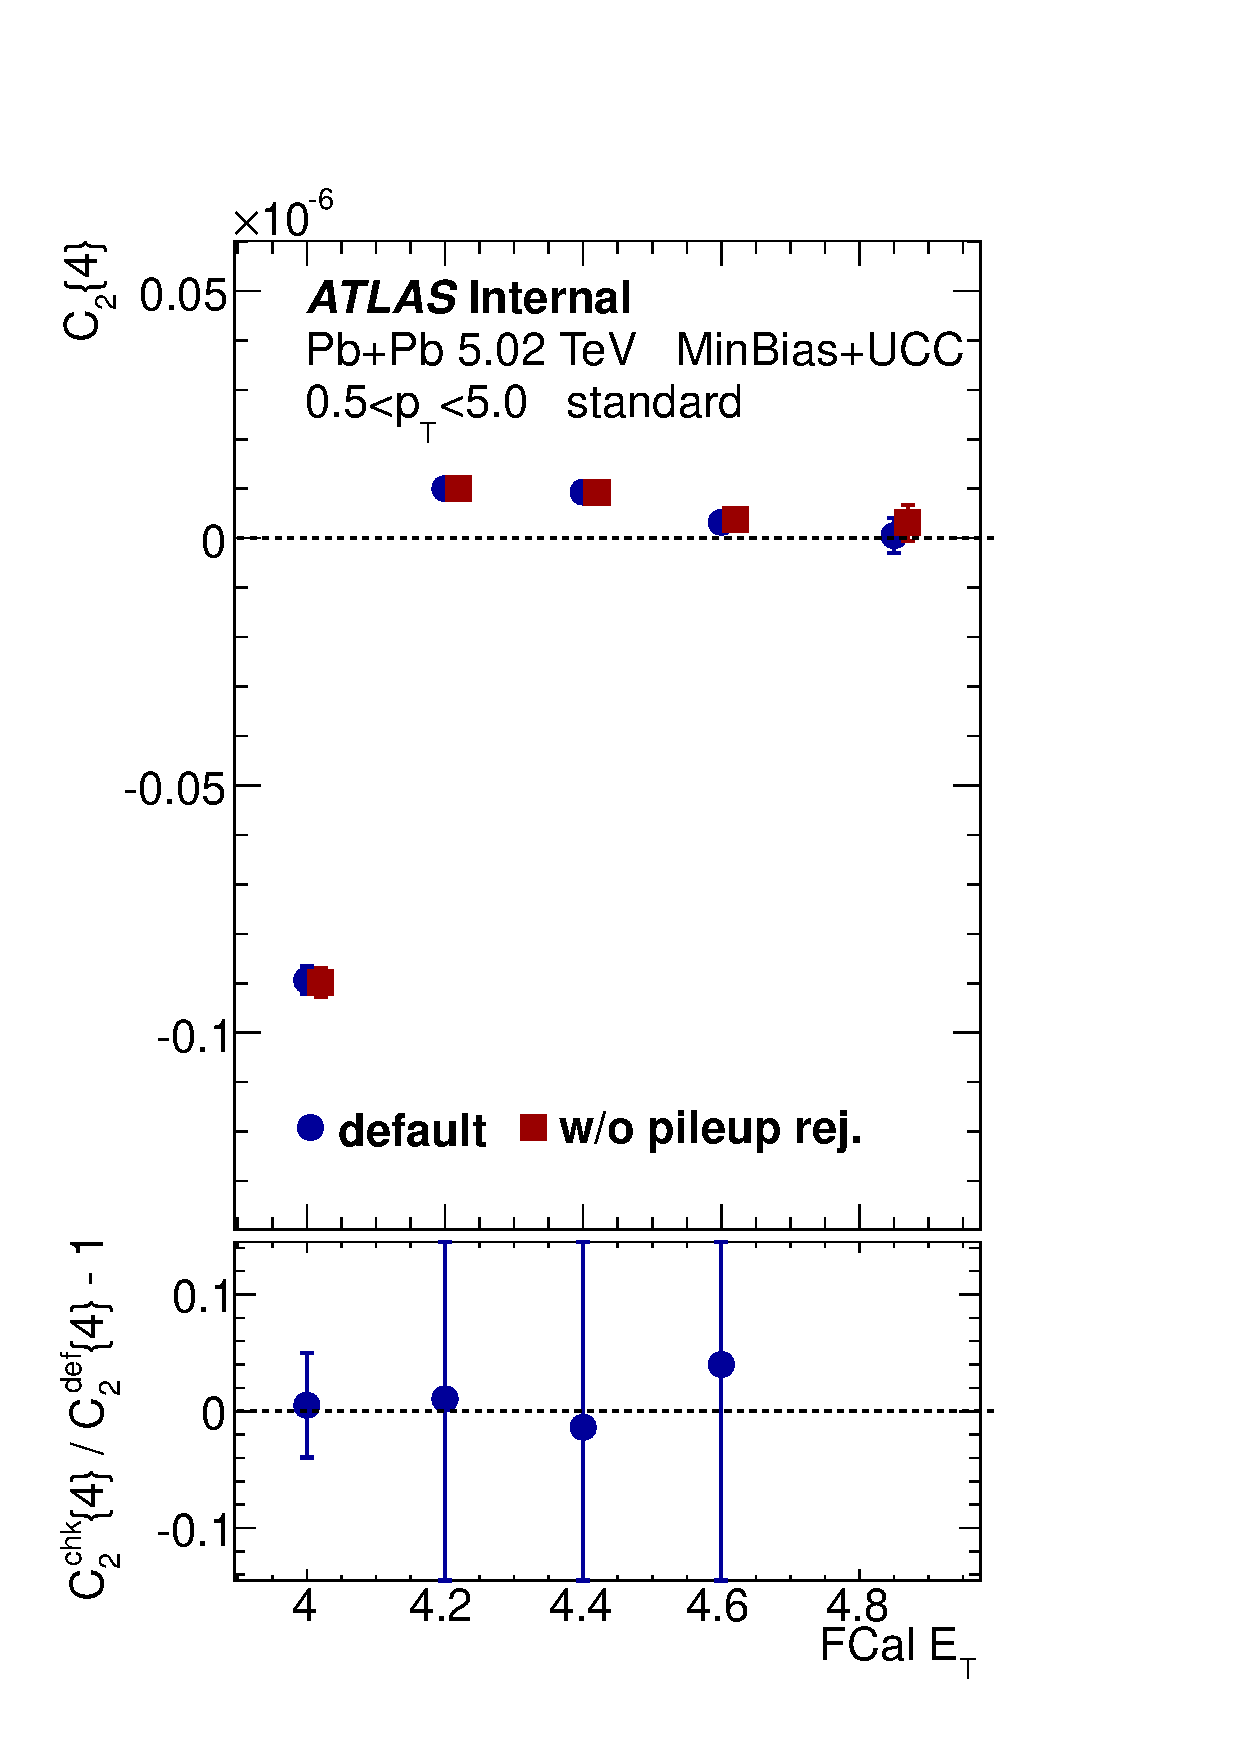
\includegraphics[width=.245\linewidth]{figs/sec_appendix/sys_PbPb502_UCC/PbPb502_sys4_1sub_Har2_Pt0.pdf}
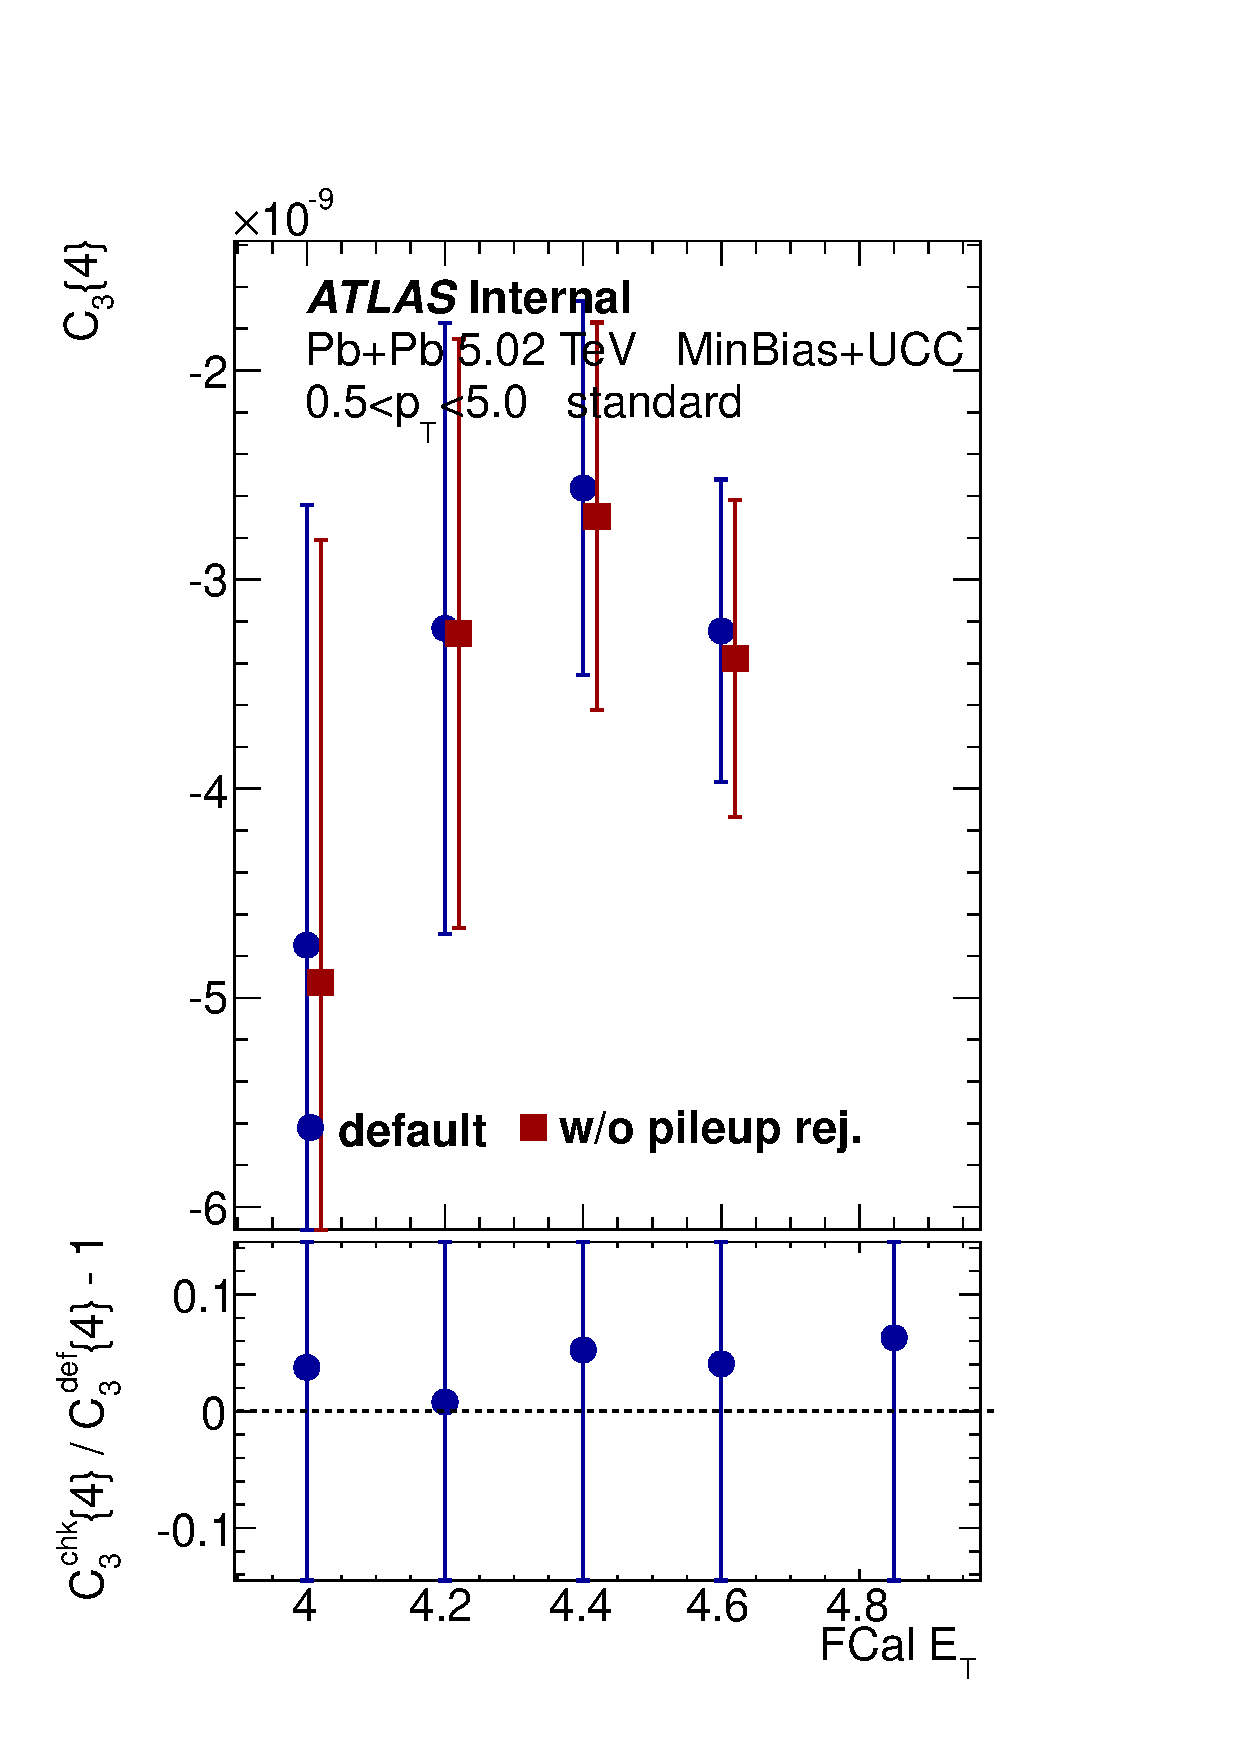
\includegraphics[width=.245\linewidth]{figs/sec_appendix/sys_PbPb502_UCC/PbPb502_sys4_1sub_Har3_Pt0.pdf}
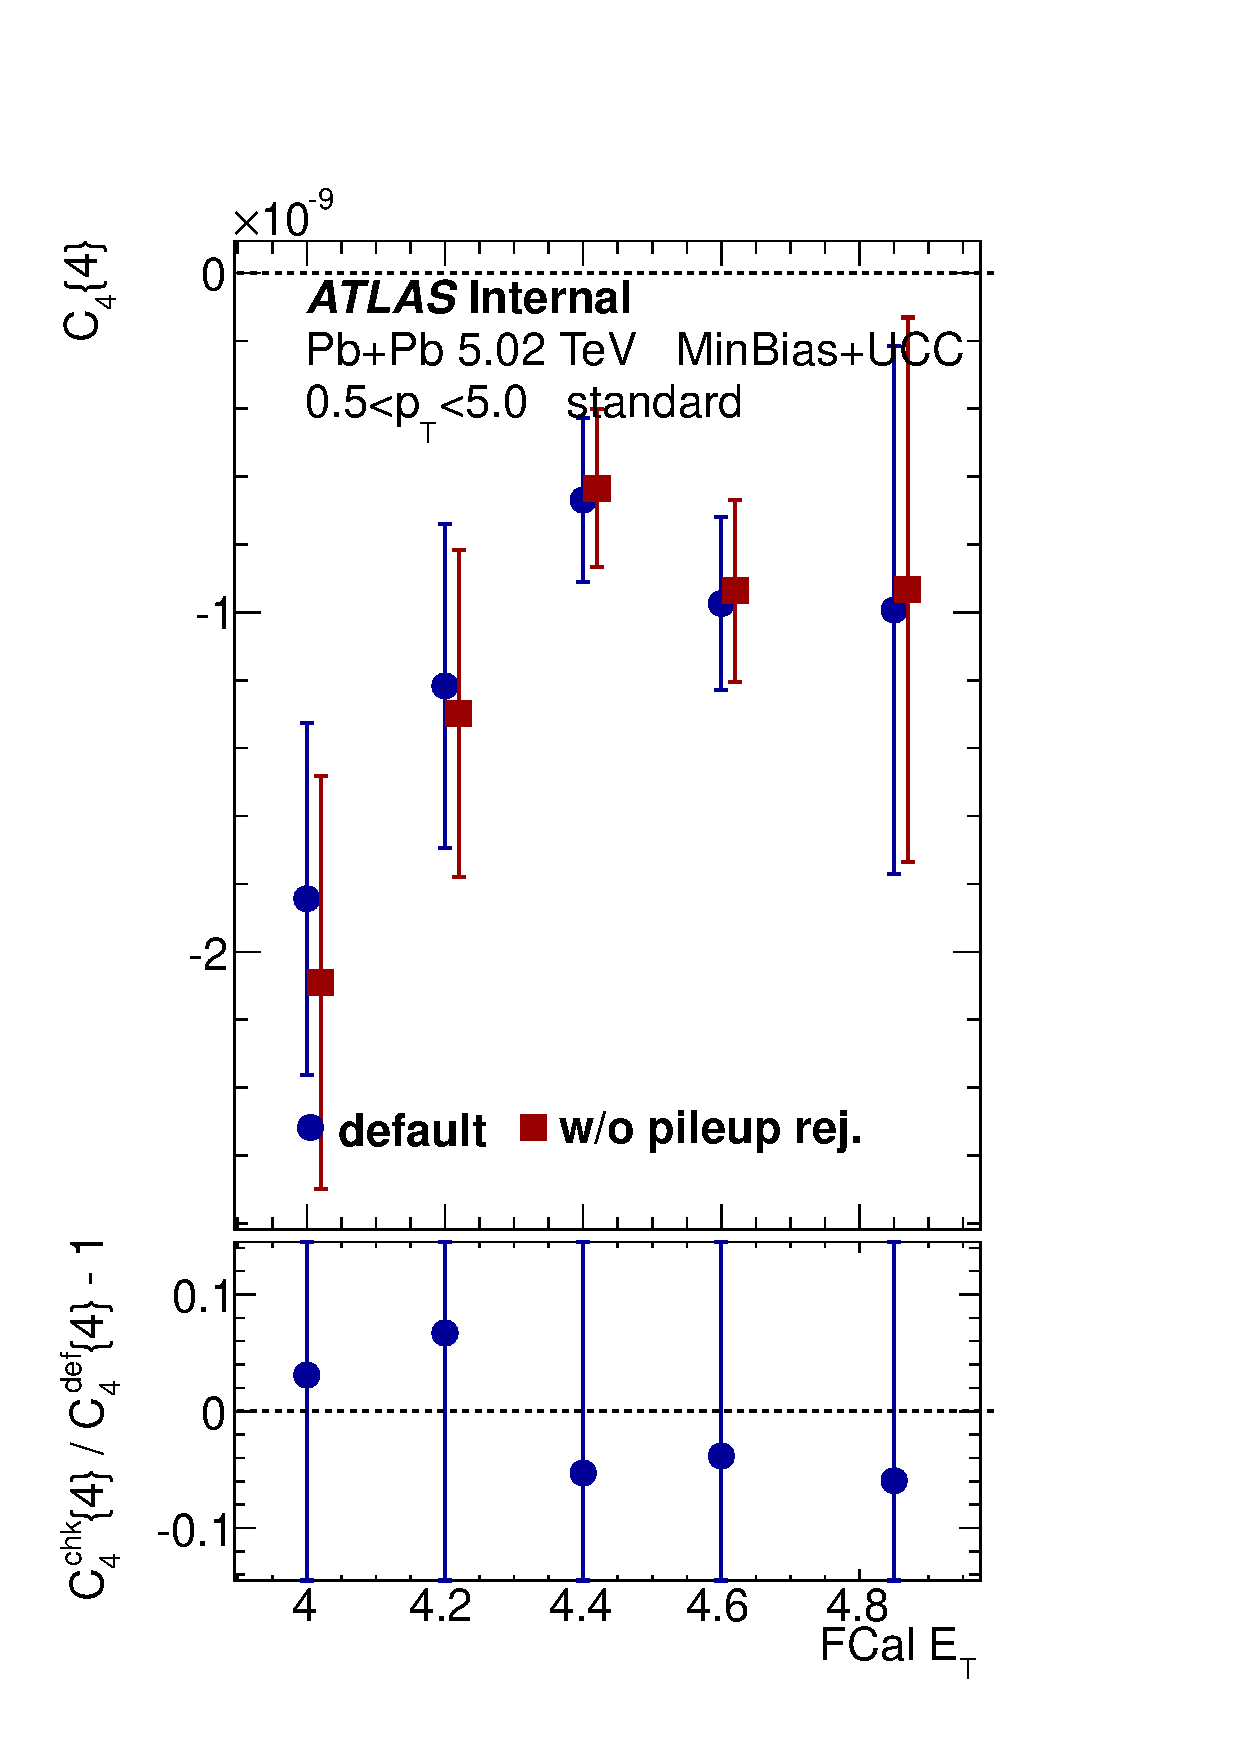
\includegraphics[width=.245\linewidth]{figs/sec_appendix/sys_PbPb502_UCC/PbPb502_sys4_1sub_Har4_Pt0.pdf}
\caption{Systematics of $c_n\{4\}$ from pileup effects: with s.s. without pileup rejection. Bottom panels are the relative uncertainties between the default and check.}
\label{fig:sys_pu}
\end{figure}



\subsection{Detector effects from flattening procedure}
Tracking efficiency weighting corrects the possible detector effects as a function of $\eta$ and $p_\text{T}$ , but the residual detector effects could still remain in the $\phi$ direction. In heavy ion collision, since the ”event plane” angle is random from event to event, the $\phi$ distribution averaged over many events should be flat and the discrepancy is due to the detector effects.

To estimate the impact from detector effects, the flattening produce was performed. The correction factor, $w_\phi$, is defined as:
\begin{equation}
w_\phi(\eta,\phi)\equiv\frac{\lr{N(\delta\eta)}}{N(\delta\eta,\delta\phi)}
\end{equation}
where $N(\delta\eta,\delta\phi)$ is the number of particles in the small $(\eta,\phi)$ phase-space window; and $\lr{N(\delta\eta)}$ is the mean number of particles in the small $\eta$ slice averaged over the whole $\phi$ range. $w_\phi$ is evaluated run-by-run, as a function of $p_\text{T}$, vertex position $z_{vtx}$ and charge, so that it can properly correct the detector effects.

To illustrate how the flattening works, Fig.~\ref{fig:sys_flat_eg} shows the $\eta-\phi$ distributions before (left) and after (right) flattening. Several holes are observed in the raw $\eta-\phi$ distribution, while after flattening, the average $\phi$ distribution is flat by construction in each $\eta$ slice.
\begin{figure}[H]
\centering
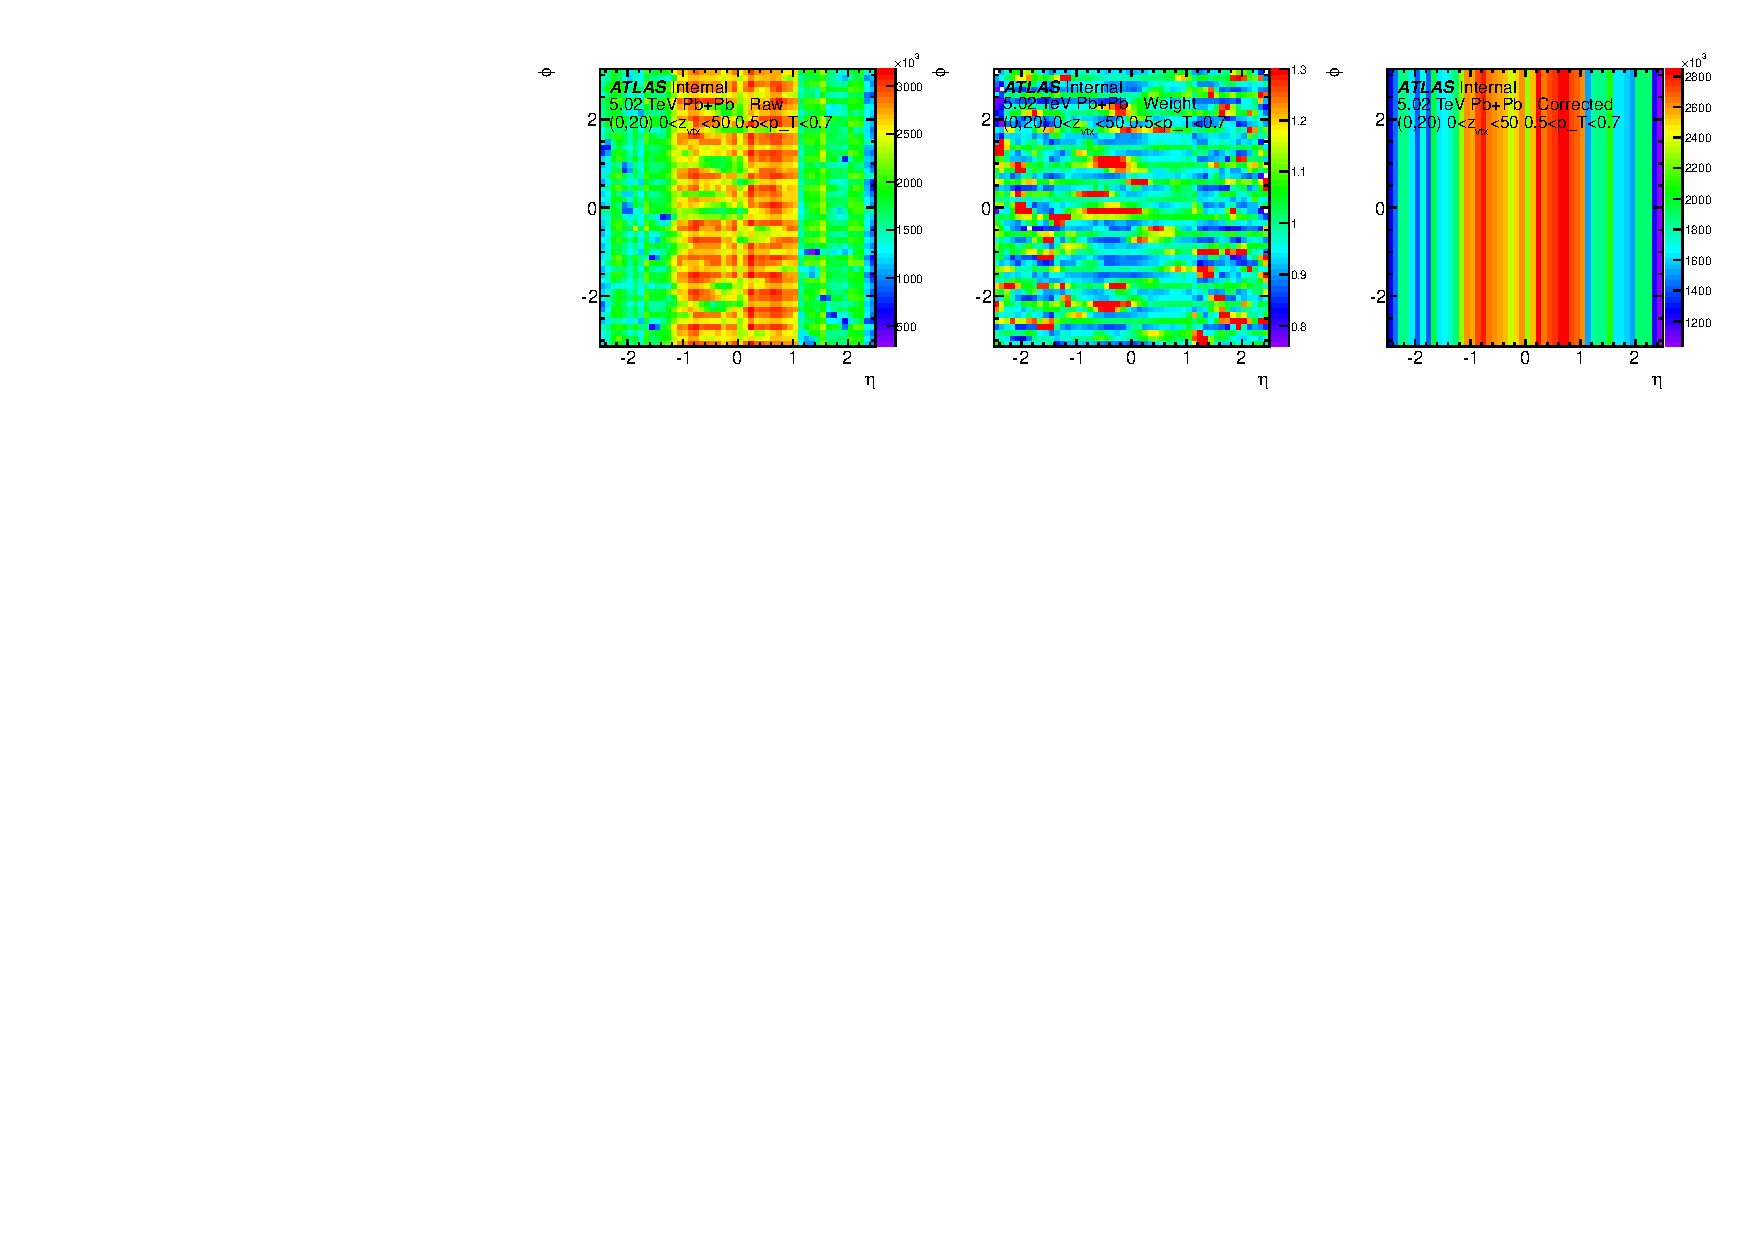
\includegraphics[width=1.\linewidth]{figs/sec_ana/cumuFlat_Cent0_Zvtx5_Chg0_Pt1.pdf}
\caption{An example demonstrating how flattening works. Left plot is the raw $\eta-\phi$ distribution, while right plot is the $\eta-\phi$ distribution after flattening procedure. Middle panel shows the correction factor $w_\phi$.}
\label{fig:sys_flat_eg}
\end{figure}

To check the impact from flattening correction, we have performed:
\begin{itemize}
\item Default: each particle weighted by $w_\phi$;
\item Check: particles not weighted by $w_\phi$;
\end{itemize}

A comparison of $c_n\{4\}$ before and after flattening is shown in Fig.~\ref{fig:sys_flat}. For all the harmonics, the relative differences are within $10\%$ and within statistical uncertainties. However, the relative difference seems to increase towards the central collision. Since the detector effect indeed depends on the occupancy of detector, it is worth checking the impact from flattening in UCC in details.
\begin{figure}[H]
\centering
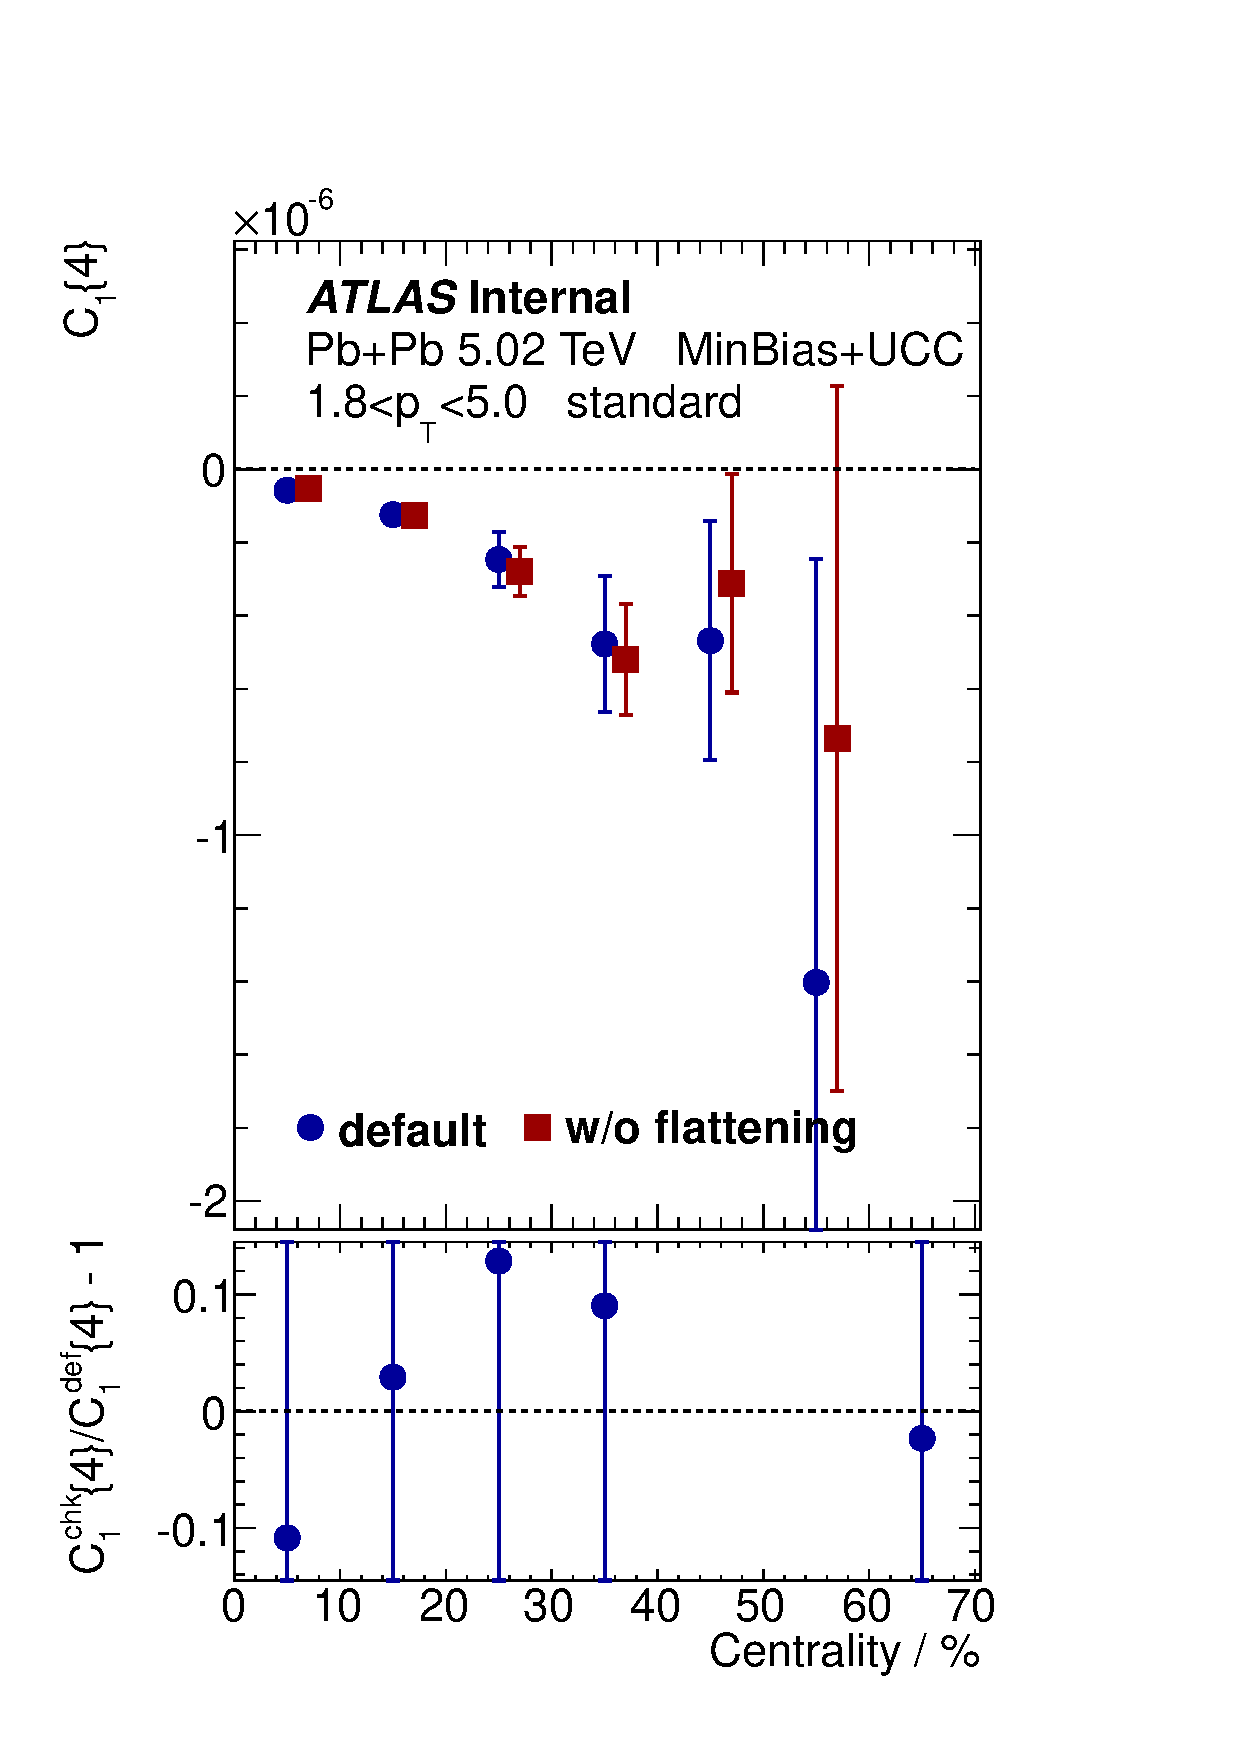
\includegraphics[width=.245\linewidth]{figs/sec_appendix/sys_PbPb502/PbPb502_sys11_1sub_Har1_Pt5.pdf}
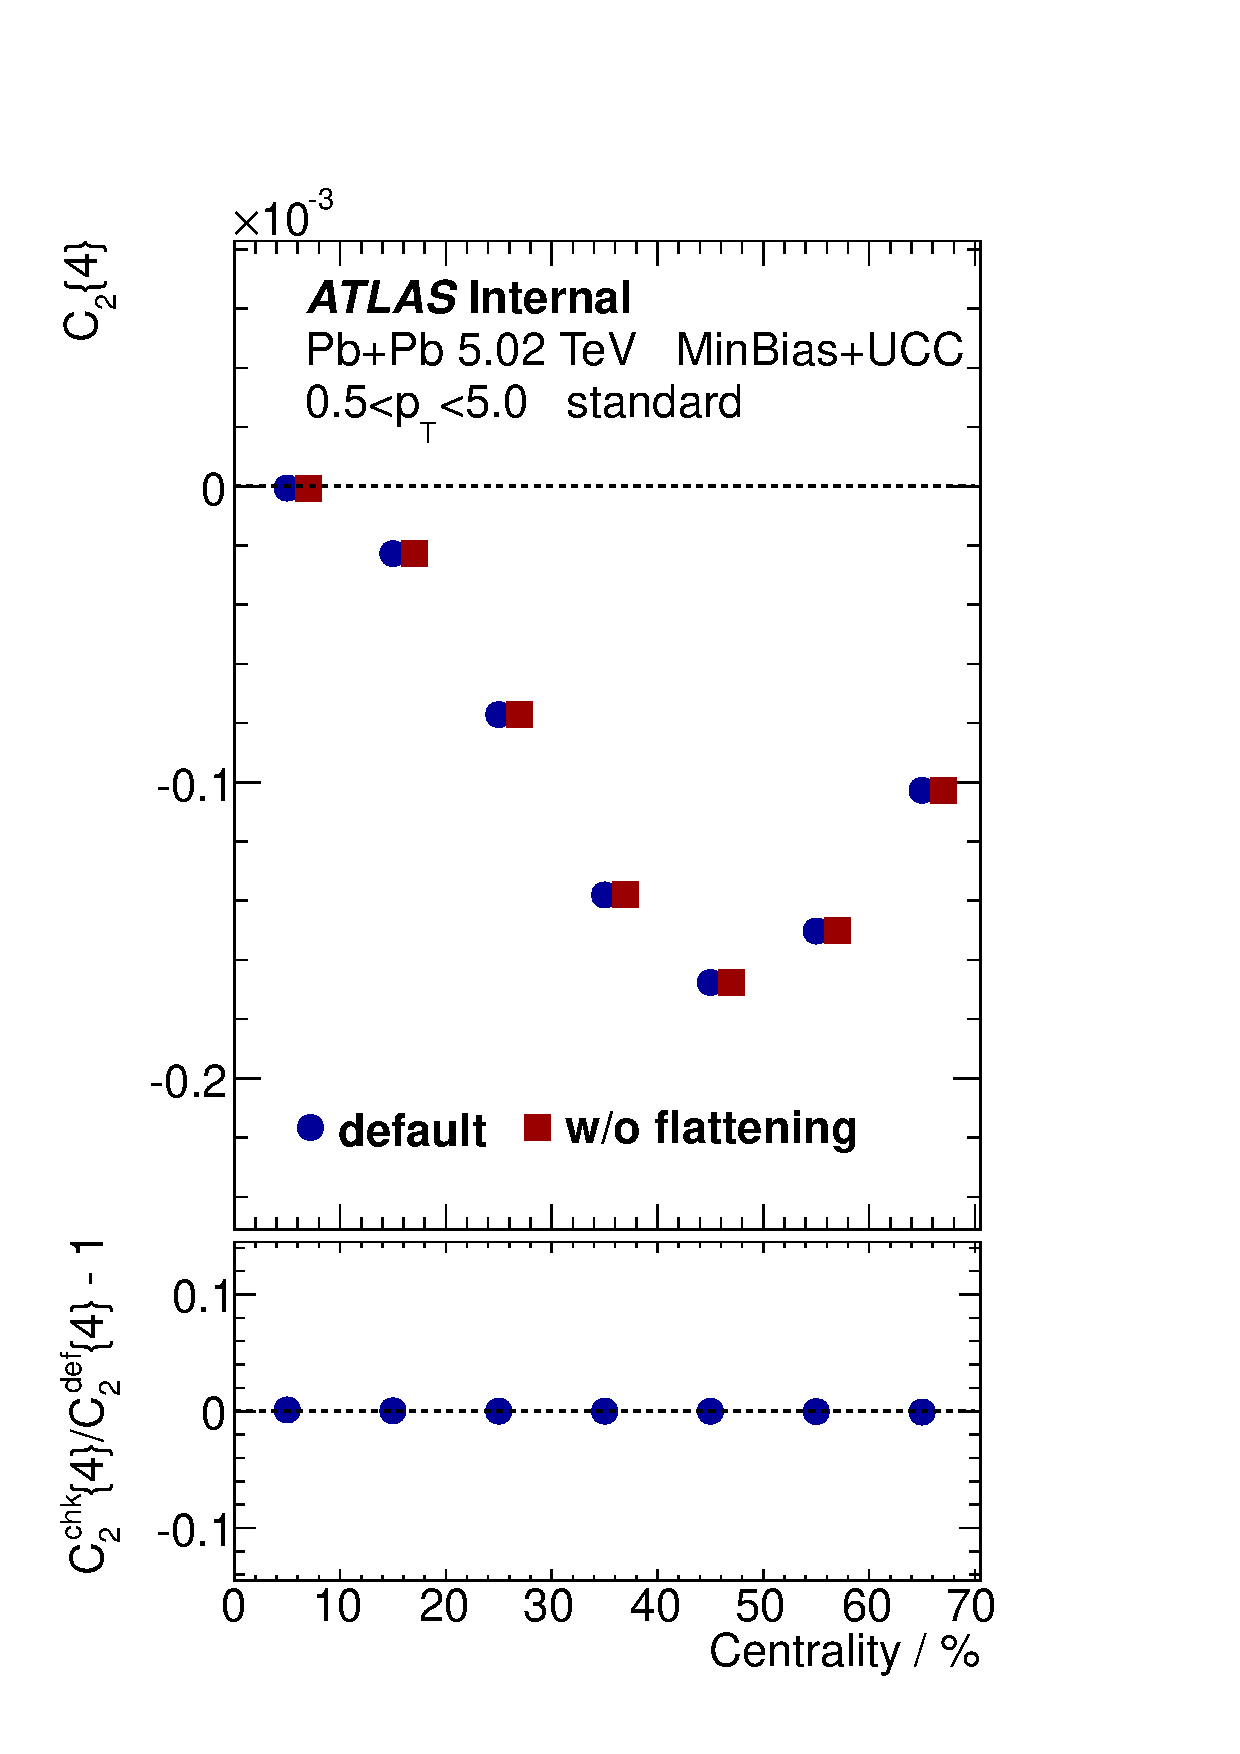
\includegraphics[width=.245\linewidth]{figs/sec_appendix/sys_PbPb502/PbPb502_sys11_1sub_Har2_Pt0.pdf}
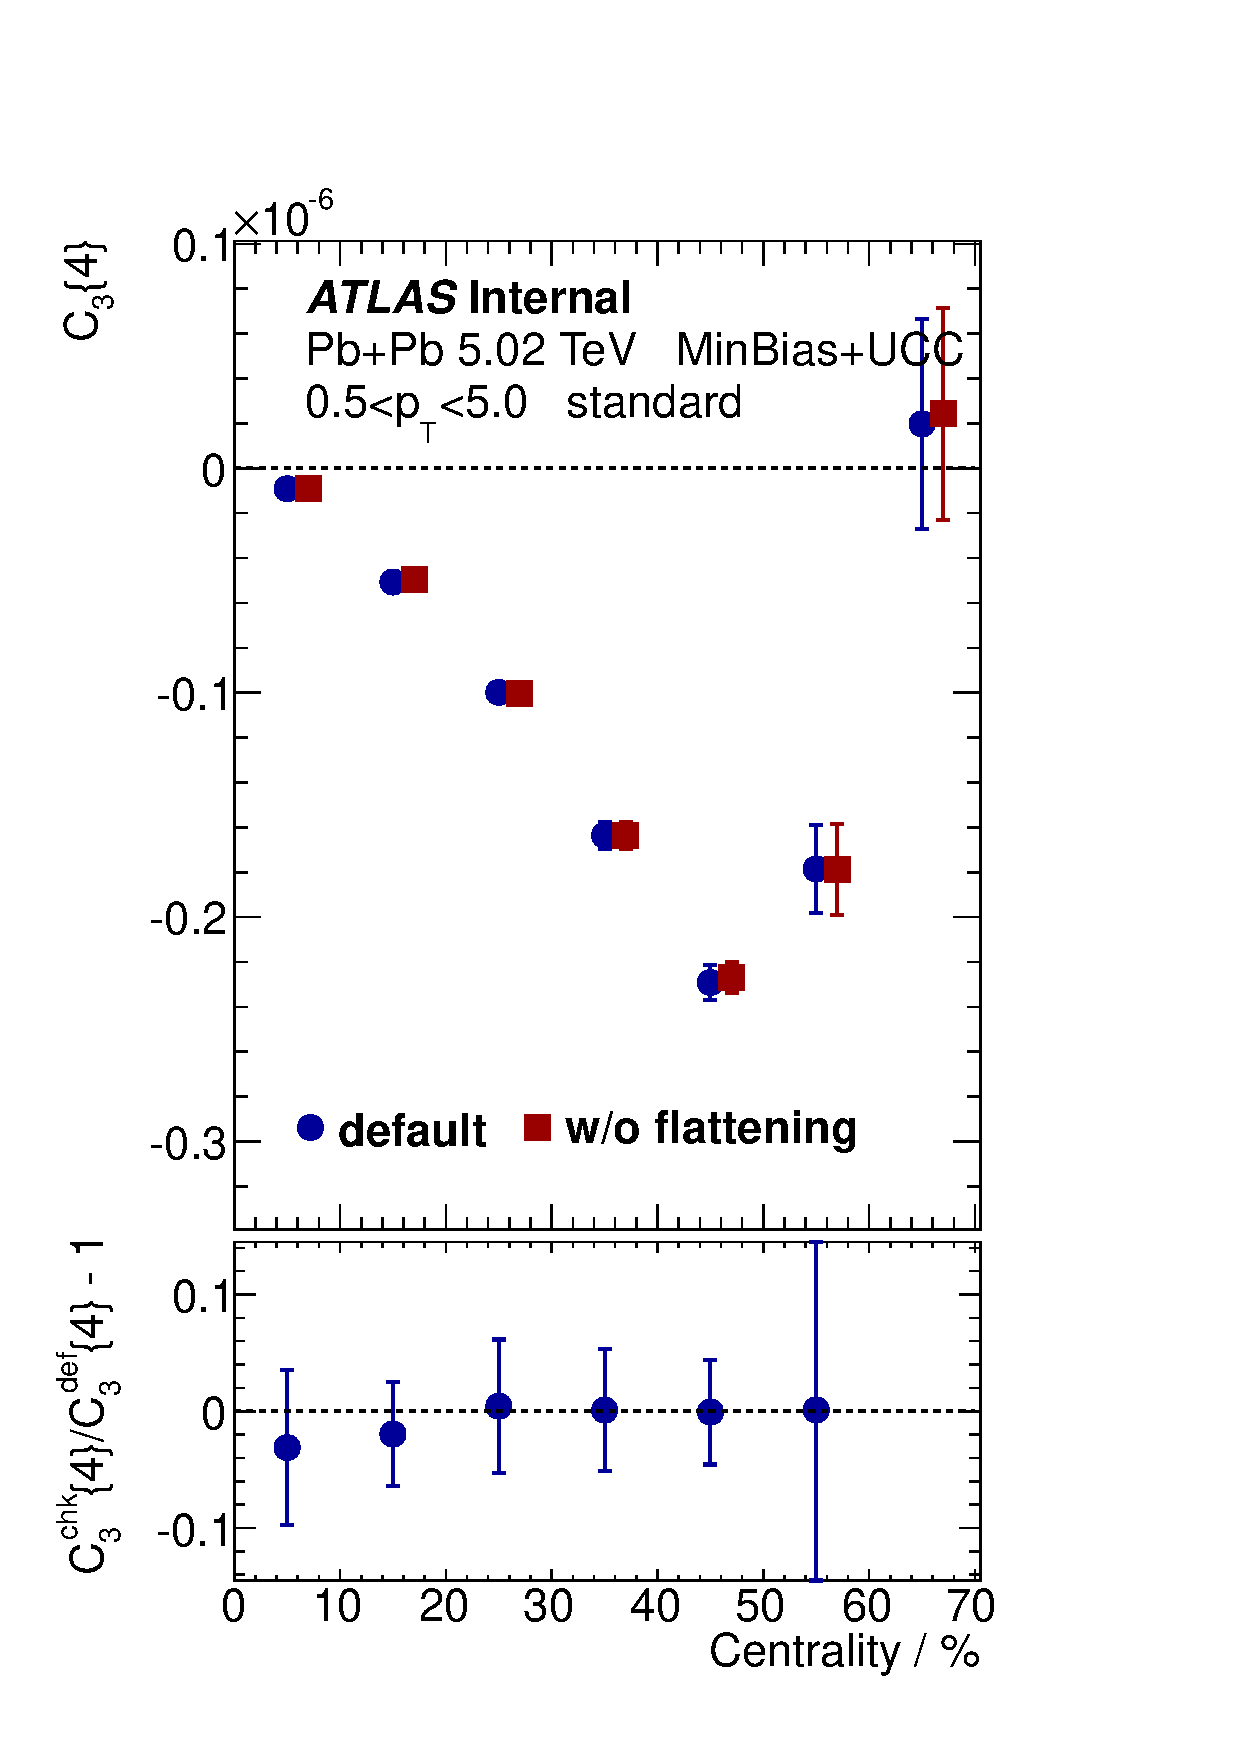
\includegraphics[width=.245\linewidth]{figs/sec_appendix/sys_PbPb502/PbPb502_sys11_1sub_Har3_Pt0.pdf}
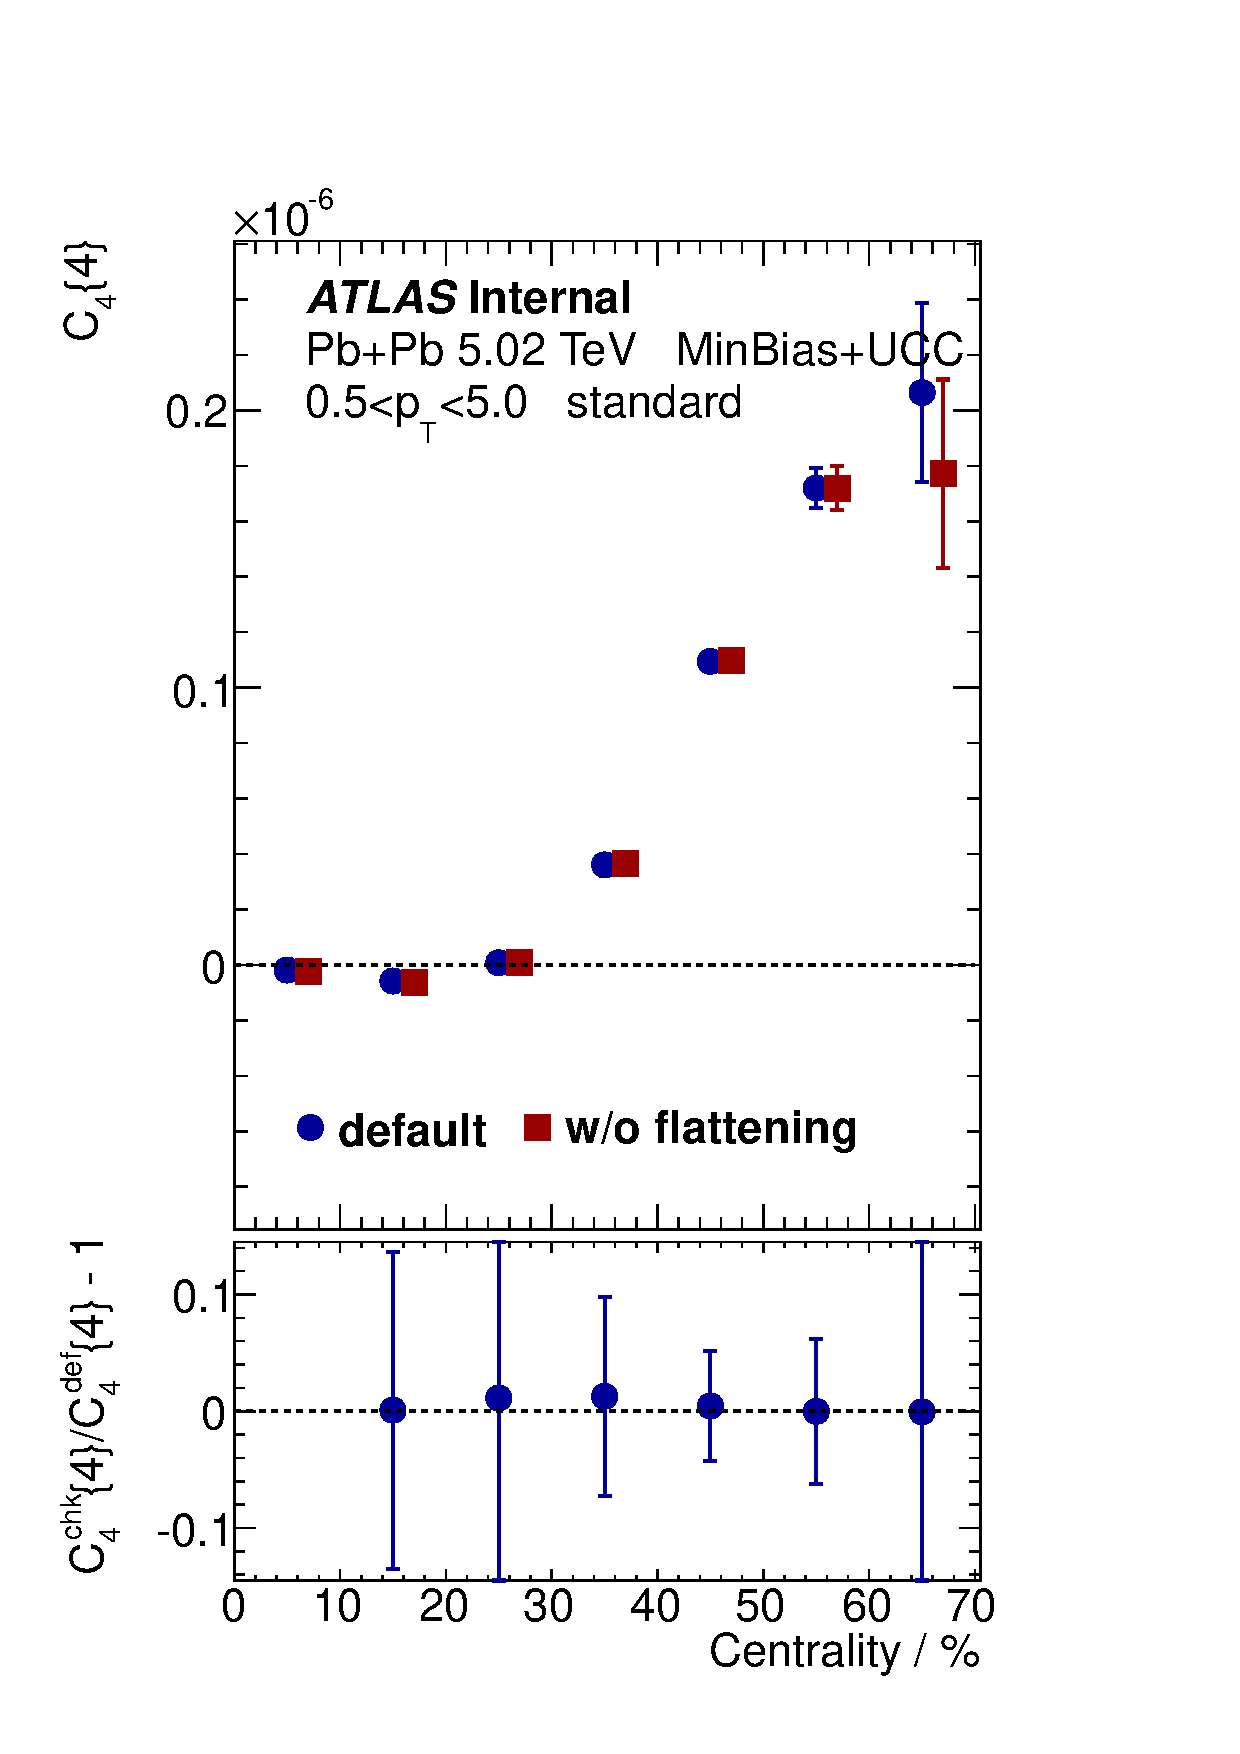
\includegraphics[width=.245\linewidth]{figs/sec_appendix/sys_PbPb502/PbPb502_sys11_1sub_Har4_Pt0.pdf}
\caption{Systematics of $c_n\{4\}$ from flattening procedure: with and without flattening. Bottom panels are the relative uncertainties between the default and check.}
\label{fig:sys_flat}
\end{figure}

A comparison of $c_n\{4\}$ in ultra-central collisions before and after flattening is shown in Fig.~\ref{fig:sys_flat_UCC}. For the odd harmonics $c_1\{4\}$ and $c_3\{4\}$, flattening does not change the results too much: the relative differences are within $10\%$ and still within statistical errors. However, for the even harmonics, especially for $c_2\{4\}$, the positive magnitude without flattening is smaller than default. Since the flattening is an essential procedure to account for the detector effects. This check will be quoted as the systematics.
\begin{figure}[H]
\centering
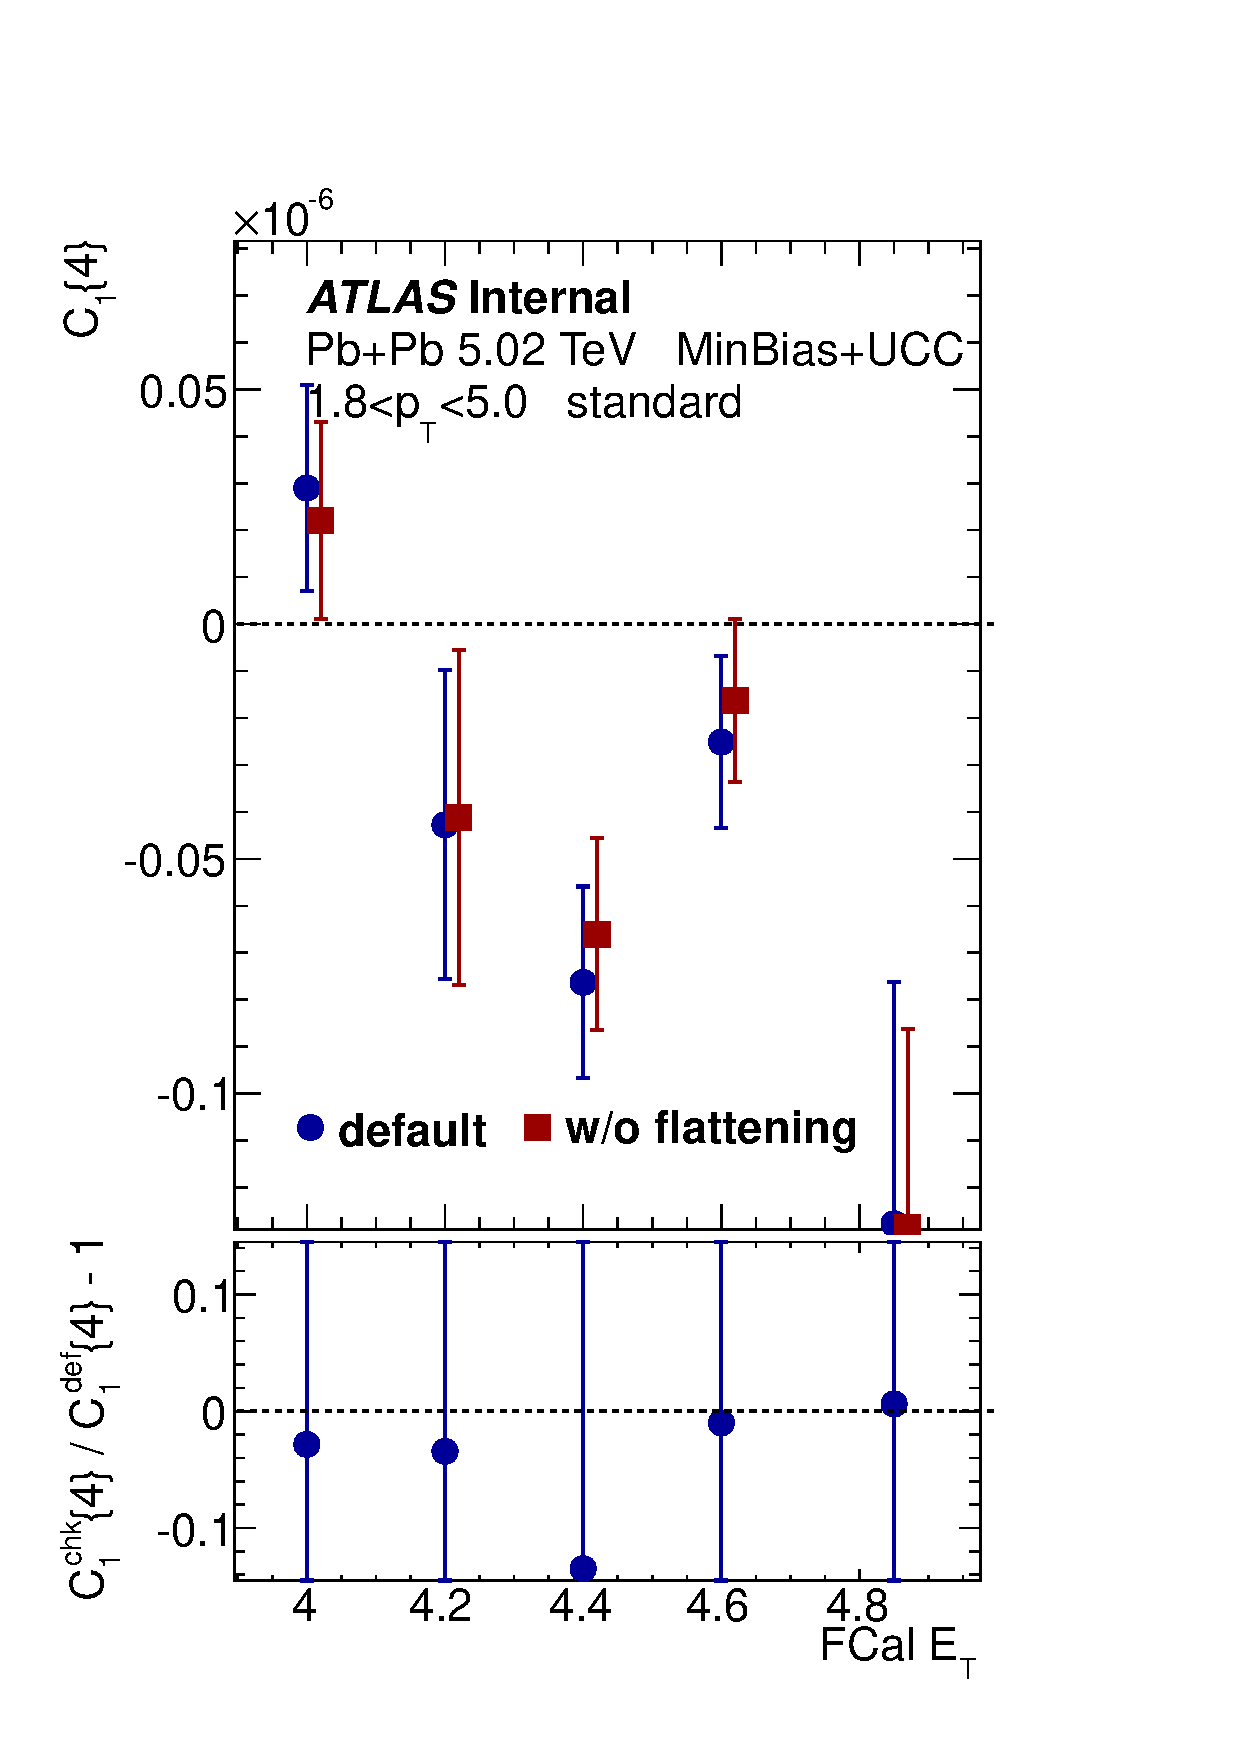
\includegraphics[width=.245\linewidth]{figs/sec_appendix/sys_PbPb502_UCC/PbPb502_sys11_1sub_Har1_Pt5.pdf}
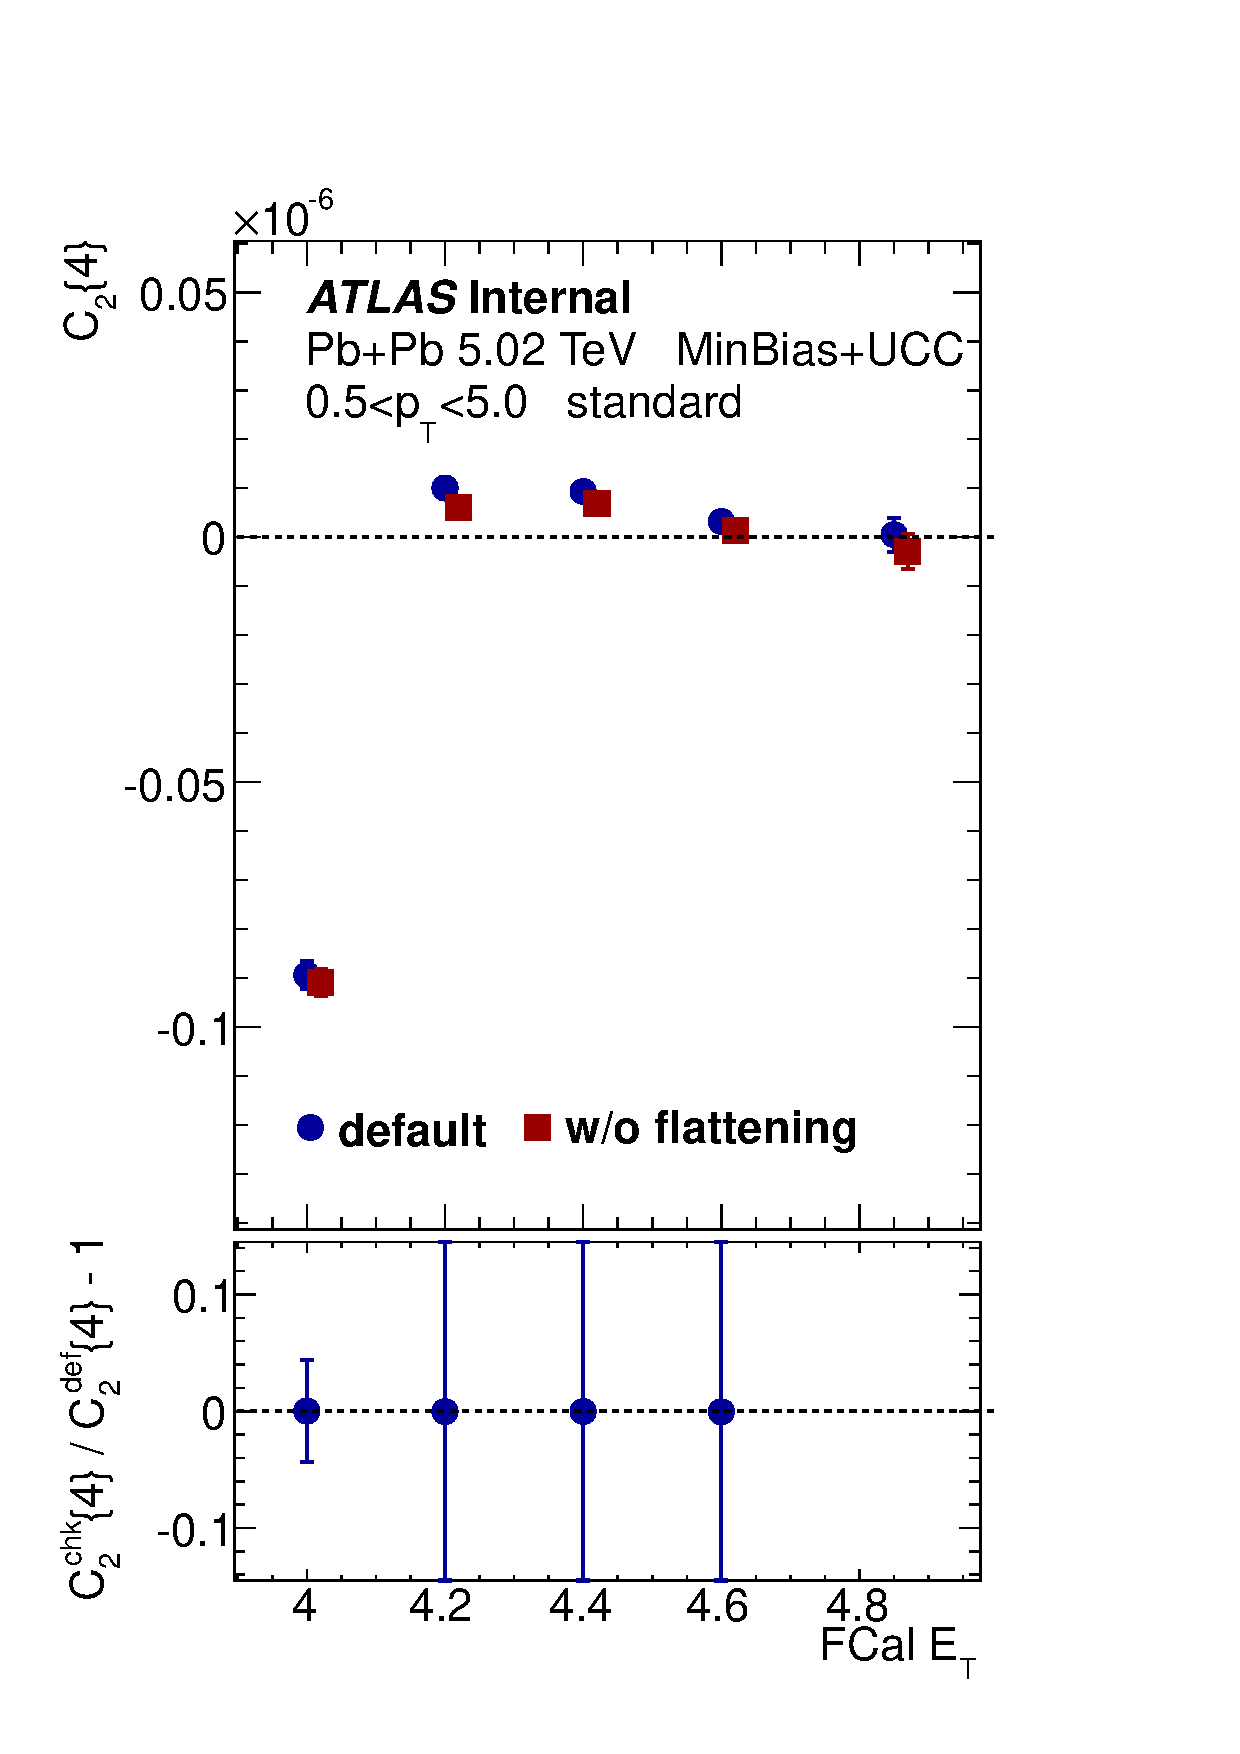
\includegraphics[width=.245\linewidth]{figs/sec_appendix/sys_PbPb502_UCC/PbPb502_sys11_1sub_Har2_Pt0.pdf}
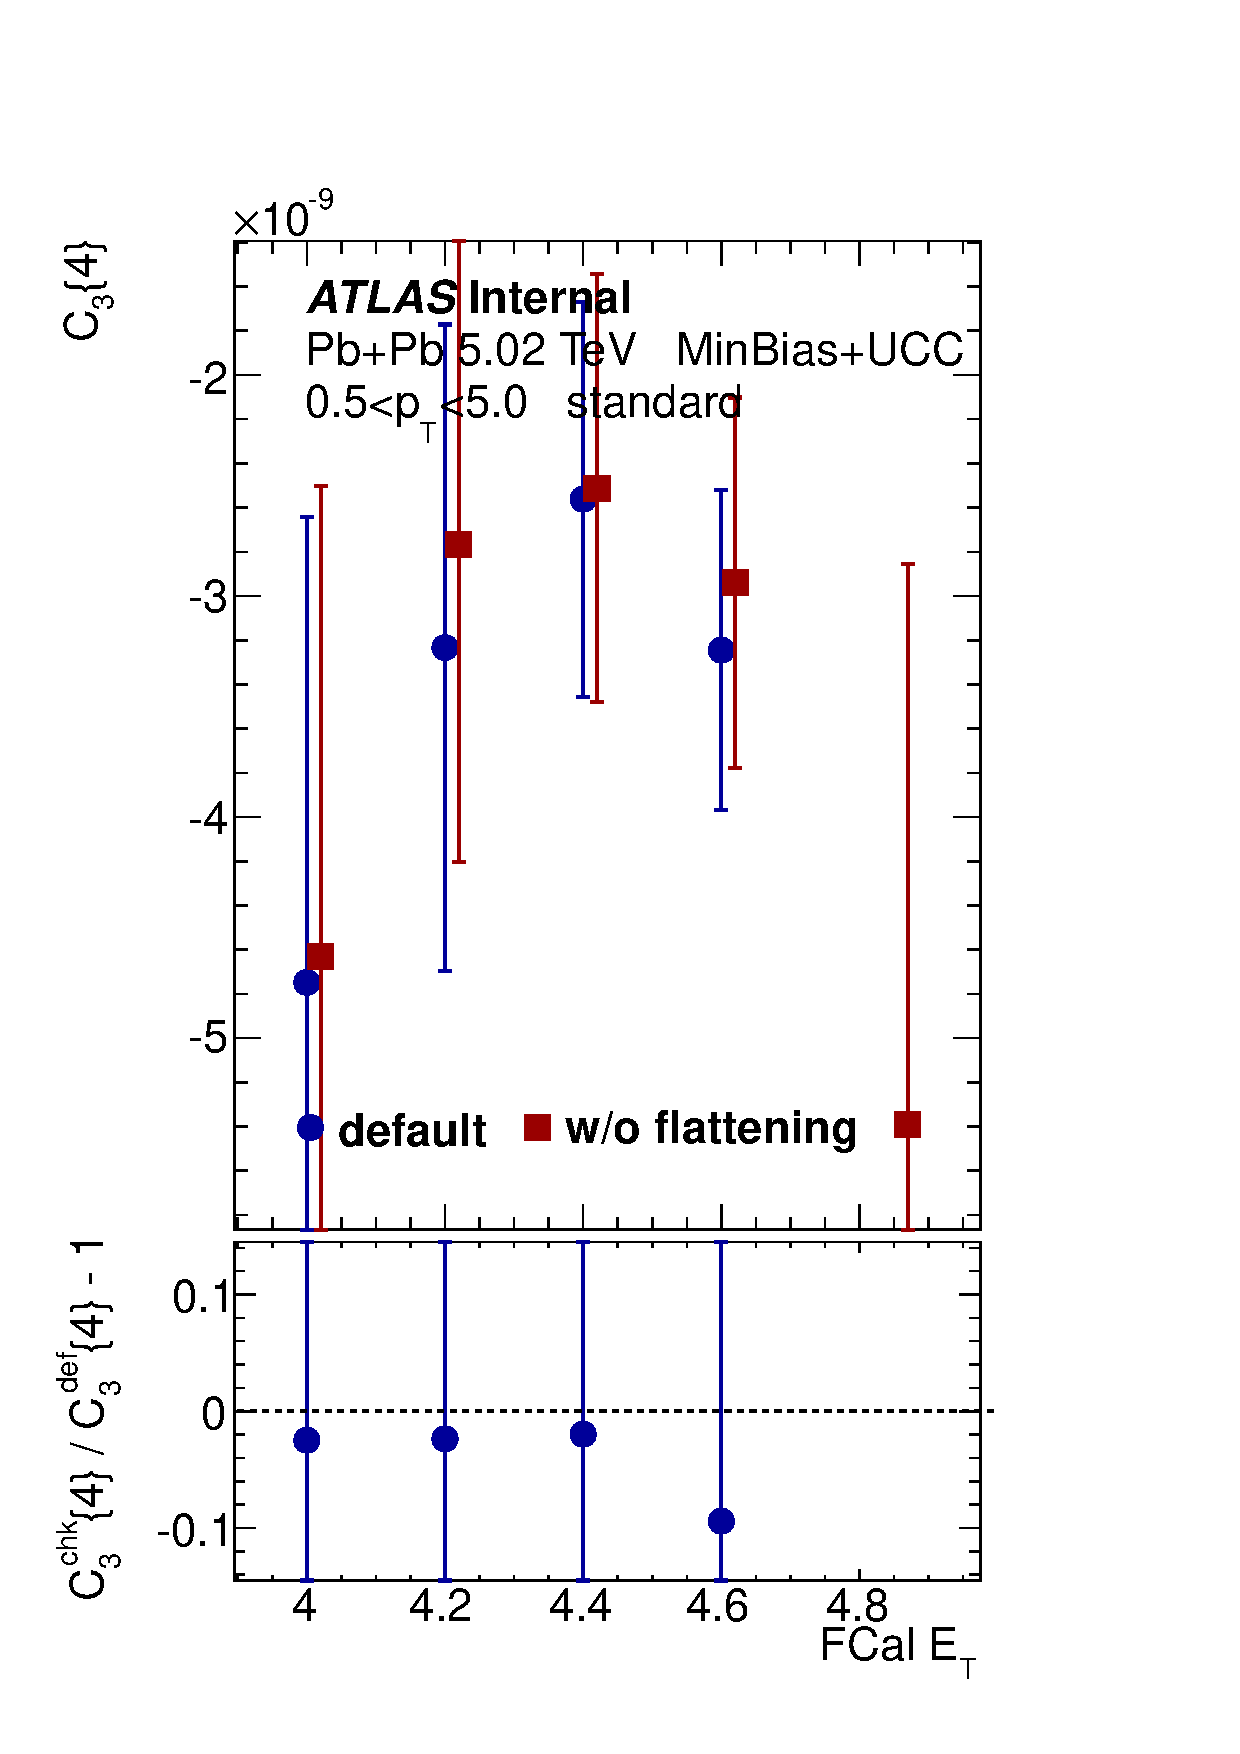
\includegraphics[width=.245\linewidth]{figs/sec_appendix/sys_PbPb502_UCC/PbPb502_sys11_1sub_Har3_Pt0.pdf}
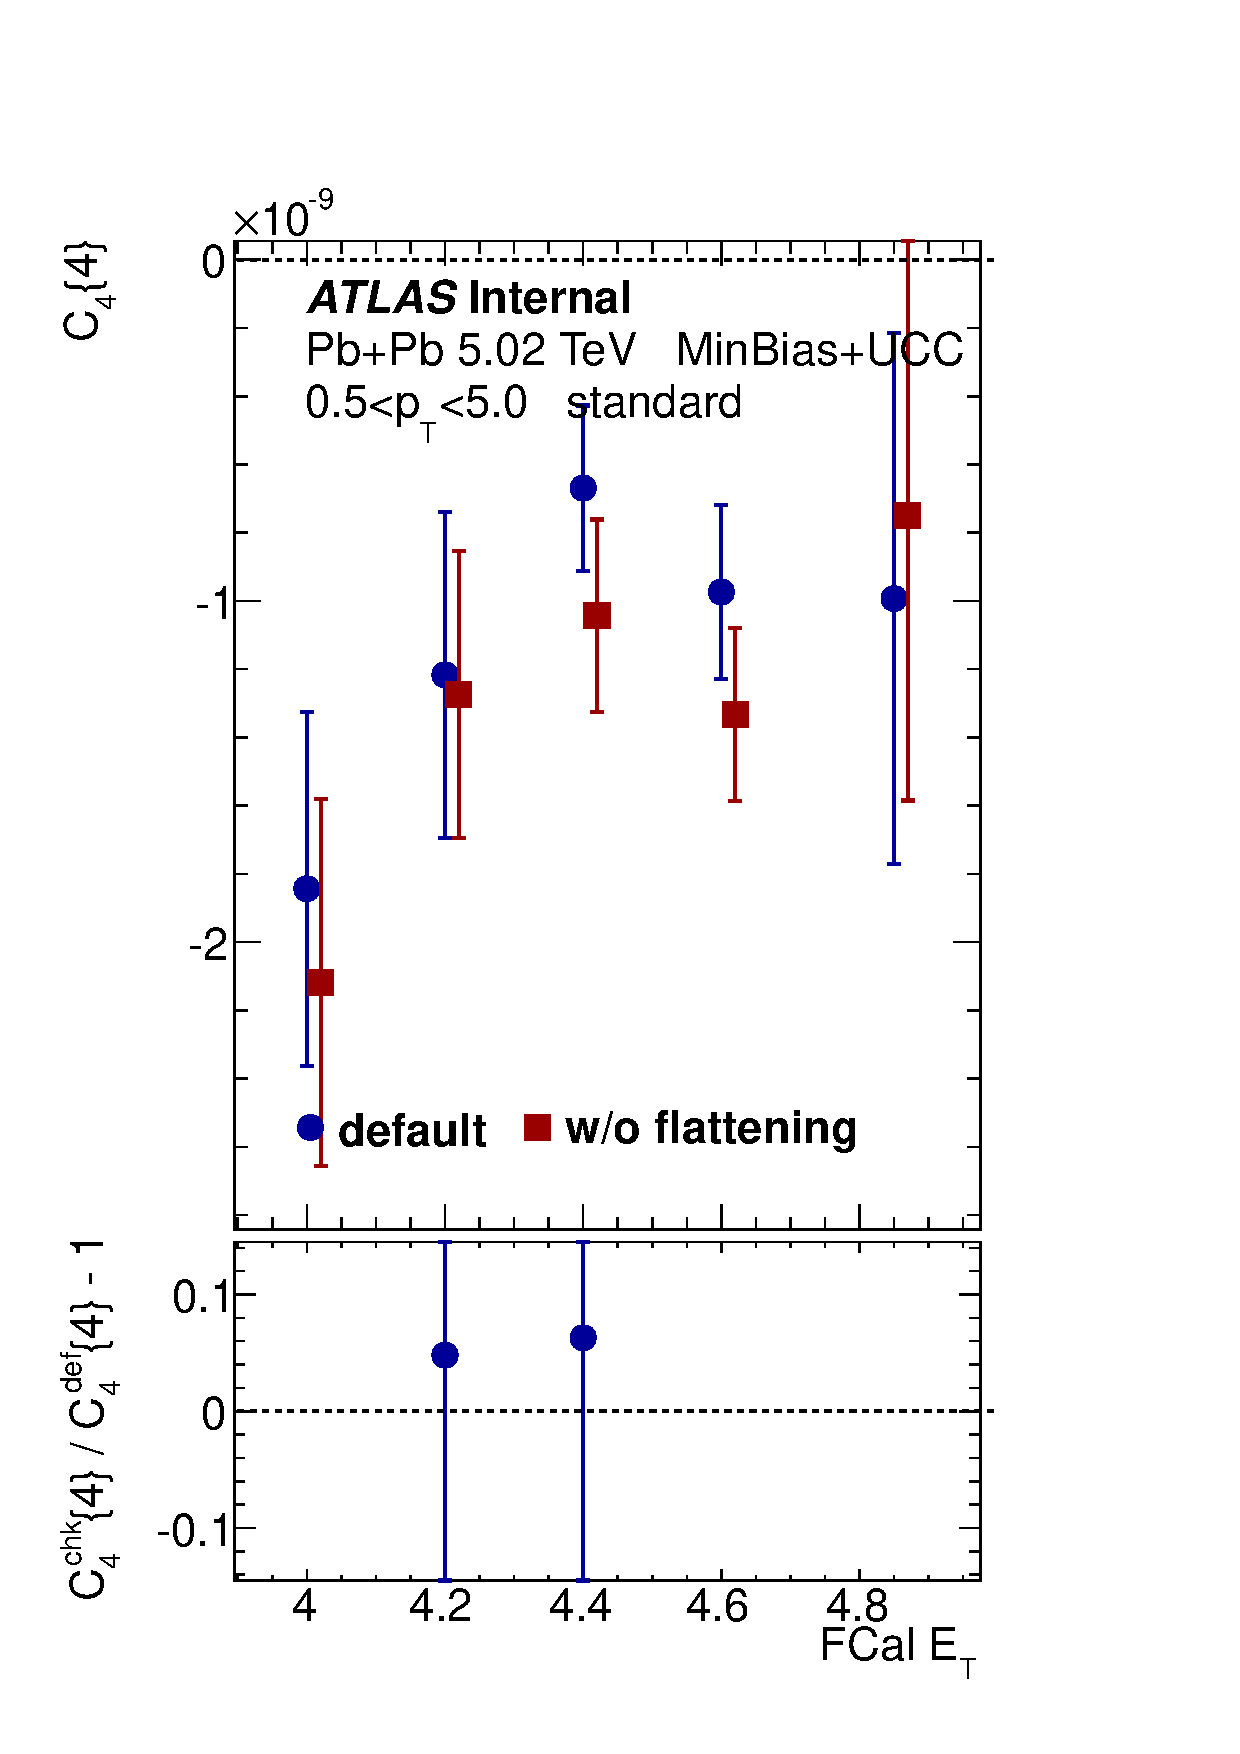
\includegraphics[width=.245\linewidth]{figs/sec_appendix/sys_PbPb502_UCC/PbPb502_sys11_1sub_Har4_Pt0.pdf}
\caption{Systematics of $c_n\{4\}$ in ultra-central collisions from flattening procedure: with and without flattening. Bottom panels are the relative uncertainties between the default and check.}
\label{fig:sys_flat_UCC}
\end{figure}

A proper way to estimate the residual detector effects after flattening should be through mixed events technique, as has been discussed in Sec.~\ref{sec:ana}.



\subsection{Centrality definition}
Uncertainty in how well the min-bias triggers sample the Pb+Pb cross-section (i.e. the min-bias trigger efficiency) results in an uncertainty in the definition of the centrality intervals. This causes the nominal $(0-85)\%$ centrality range to have a $\pm 1\%$ uncertainty. The effect of such uncertainties on observables are determined by re-evaluating the observables with the following criteria:
\begin{itemize}
\item Default: $(0-85)\%$ centrality range;
\item Check 1: $(0-84)\%$ centrality range;
\item Check 2: $(0-86)\%$ centrality range;
\end{itemize}

\begin{figure}[H]
\centering
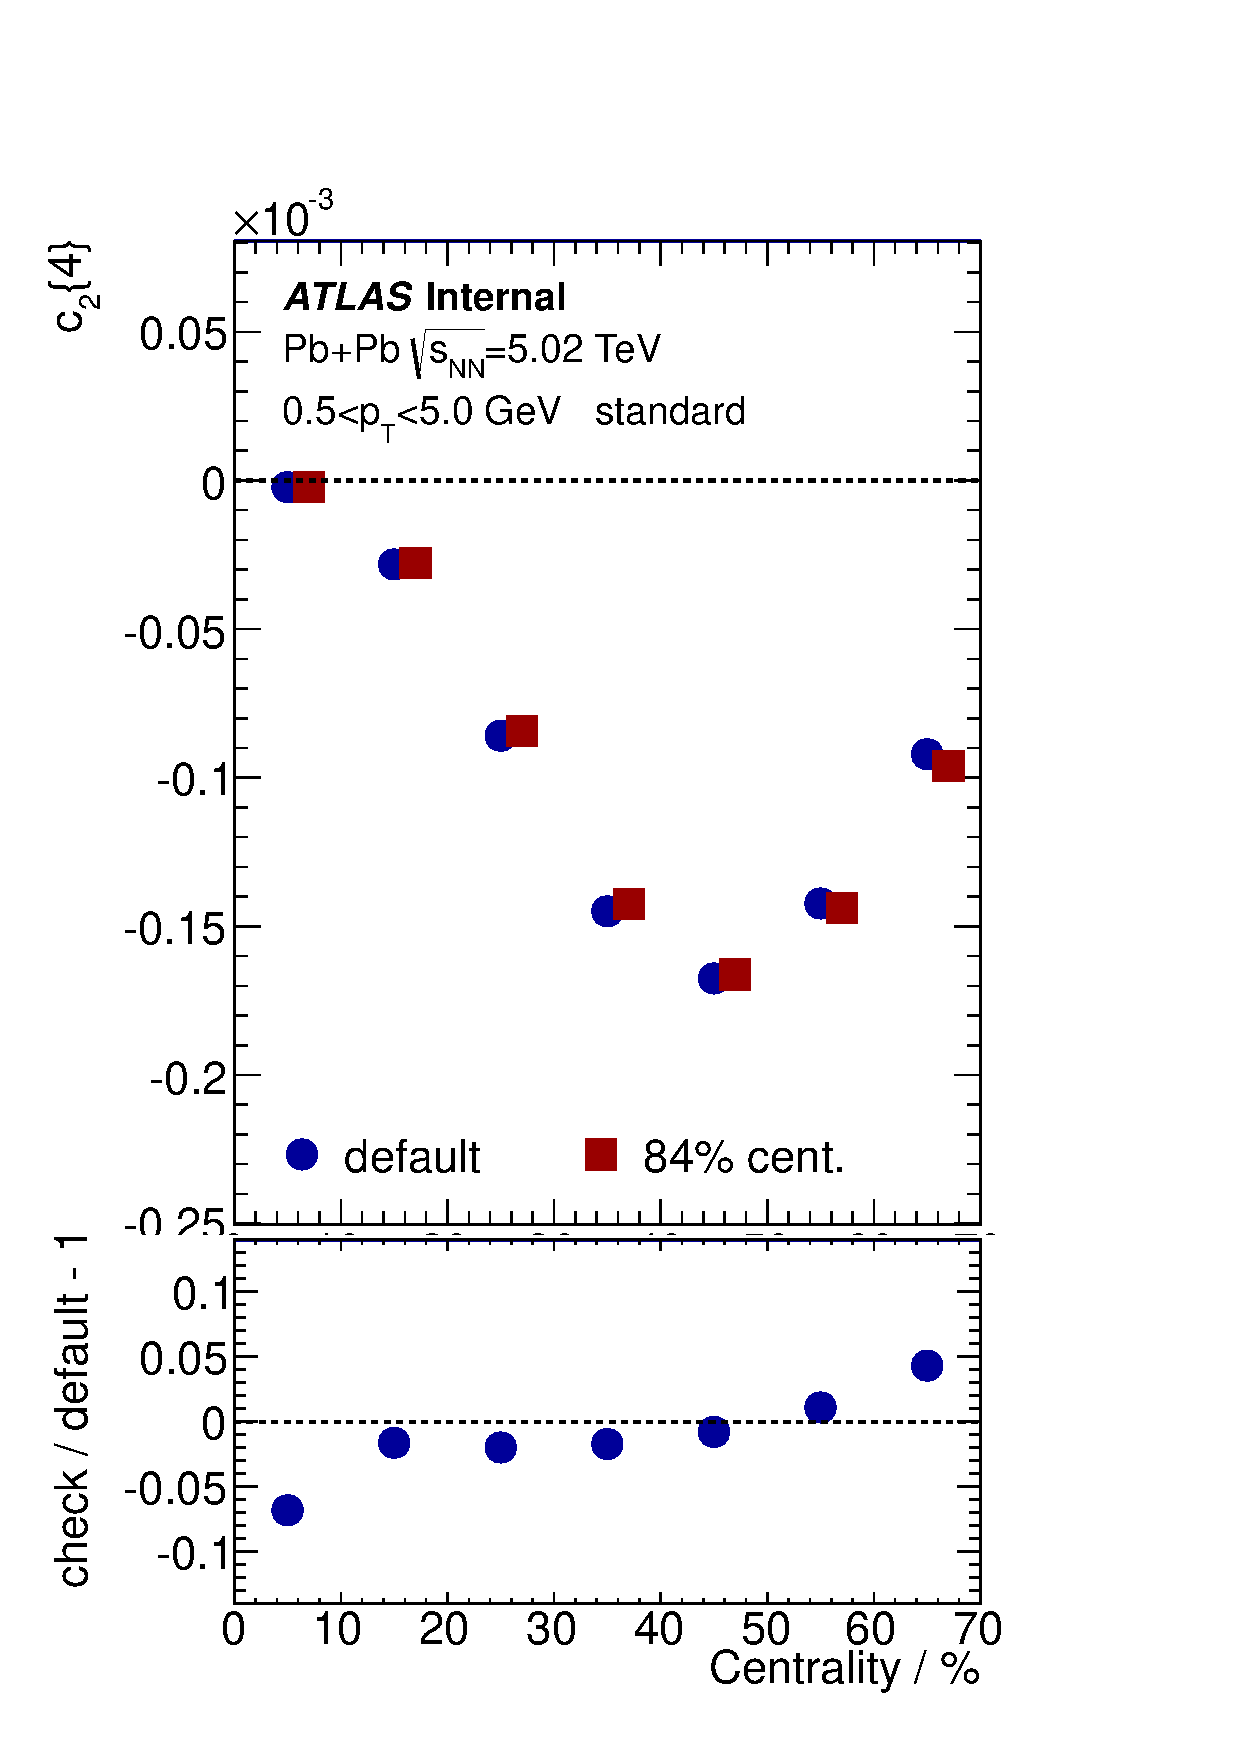
\includegraphics[width=.245\linewidth]{figs/sec_sys/summary/sys7_c4_1sub_Har2_Pt0.pdf}
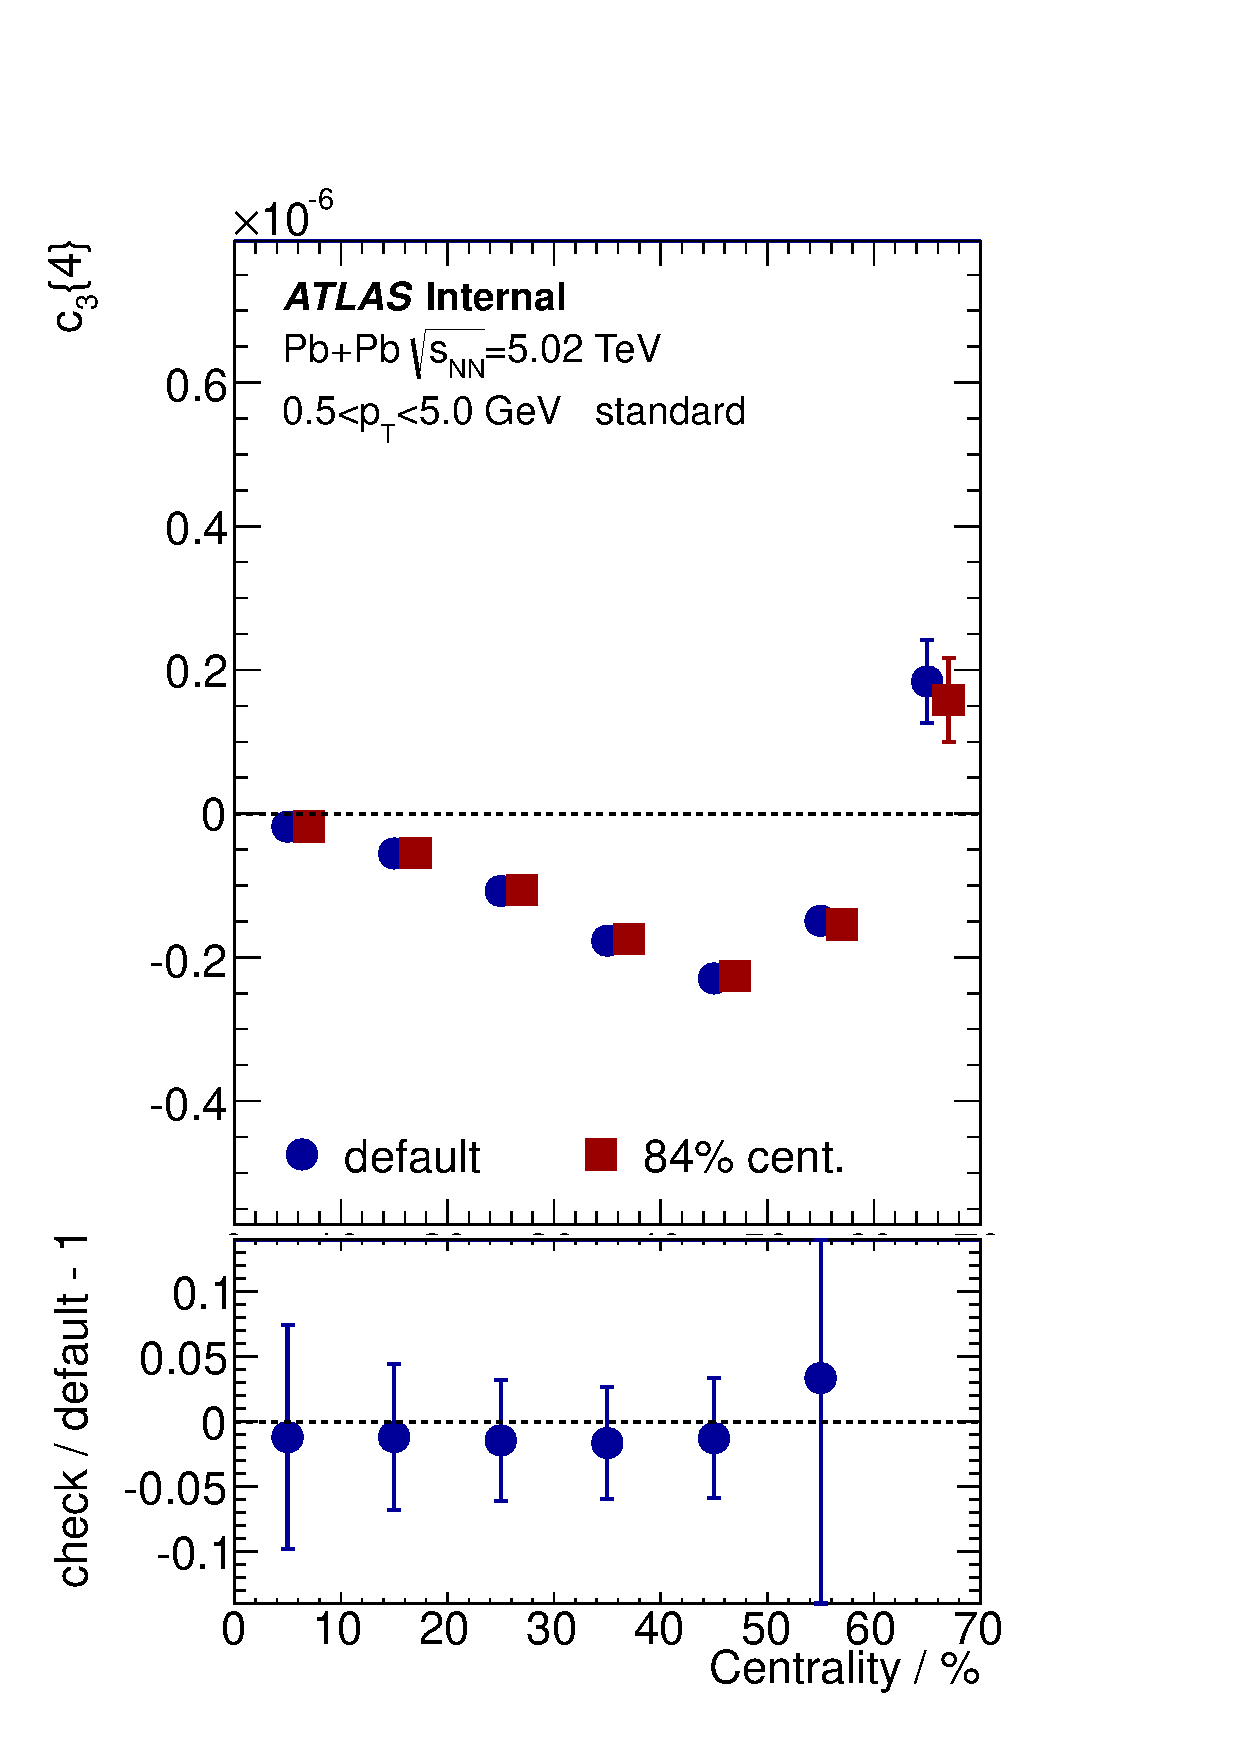
\includegraphics[width=.245\linewidth]{figs/sec_sys/summary/sys7_c4_1sub_Har3_Pt0.pdf}
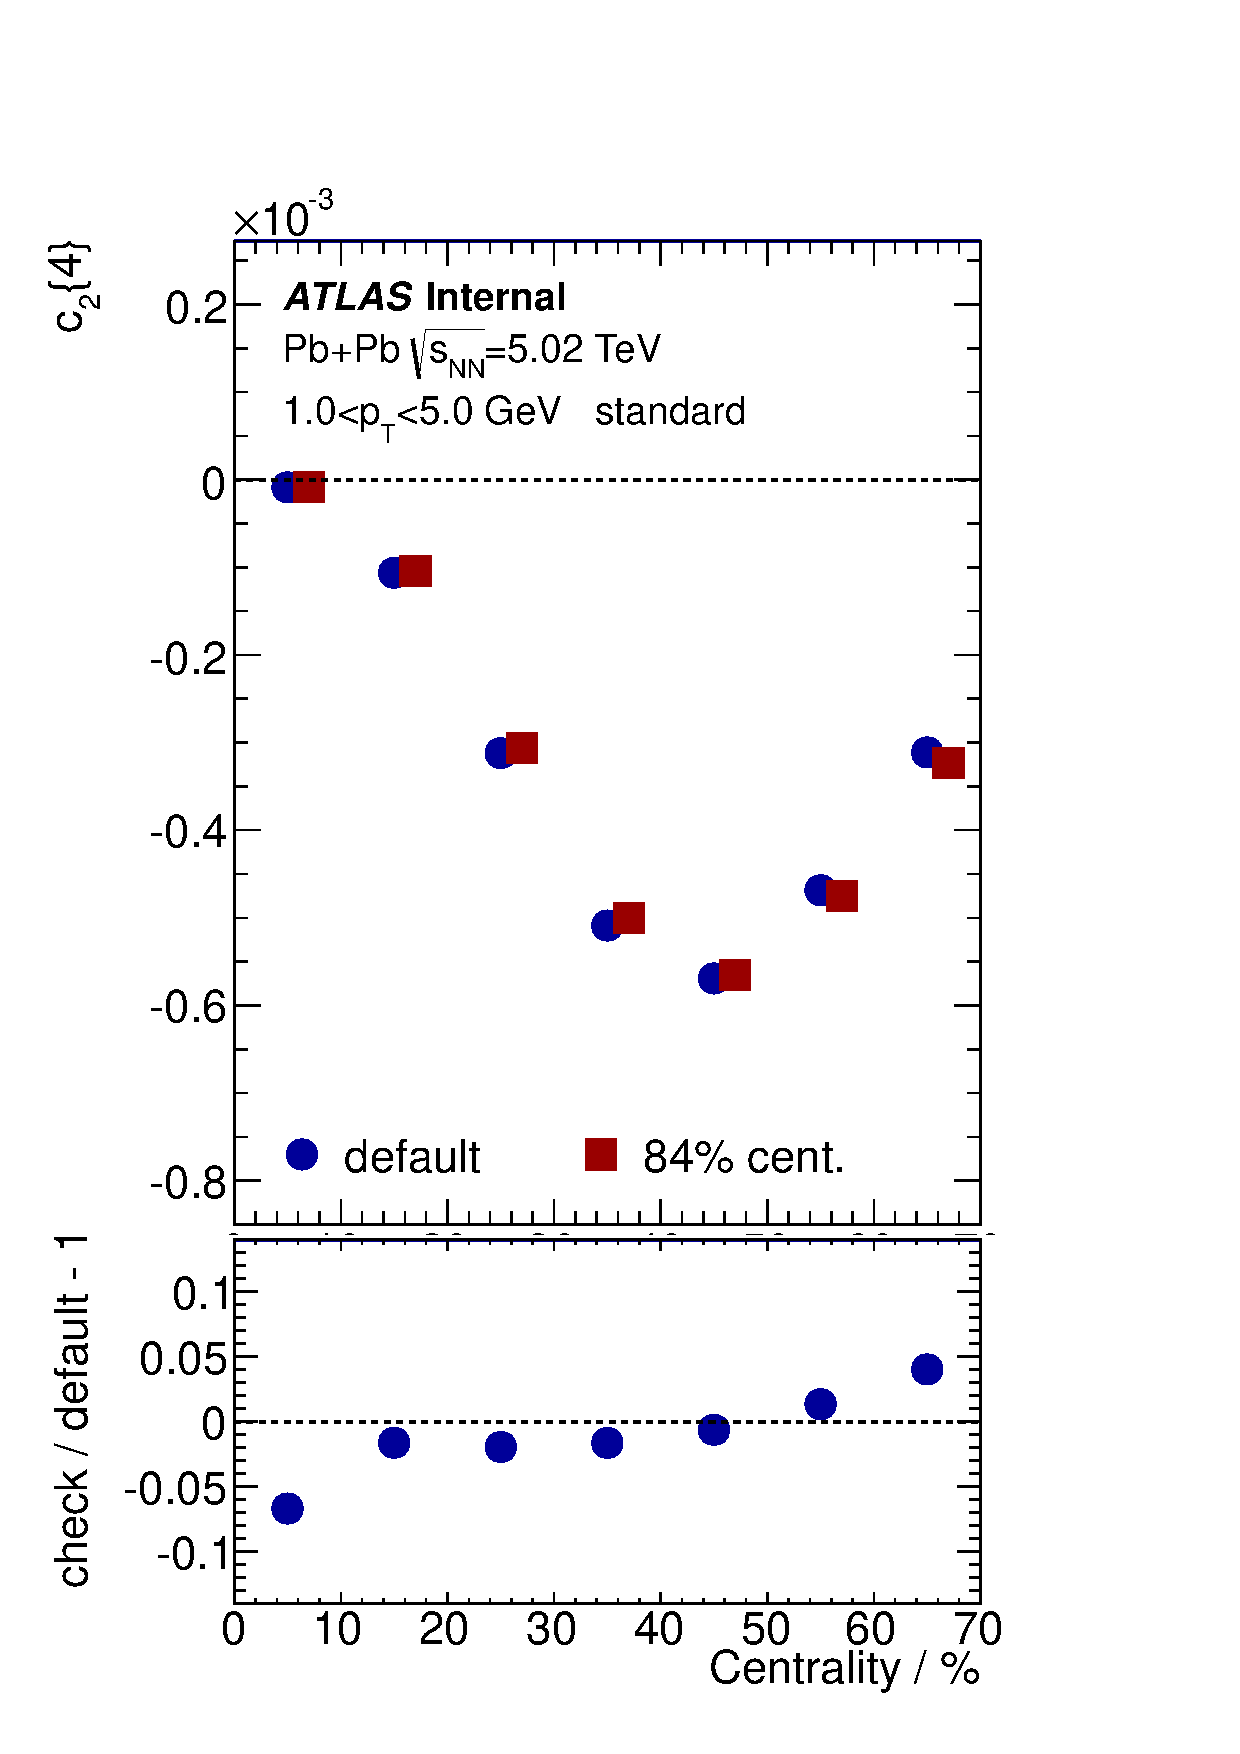
\includegraphics[width=.245\linewidth]{figs/sec_sys/summary/sys7_c4_1sub_Har2_Pt1.pdf}
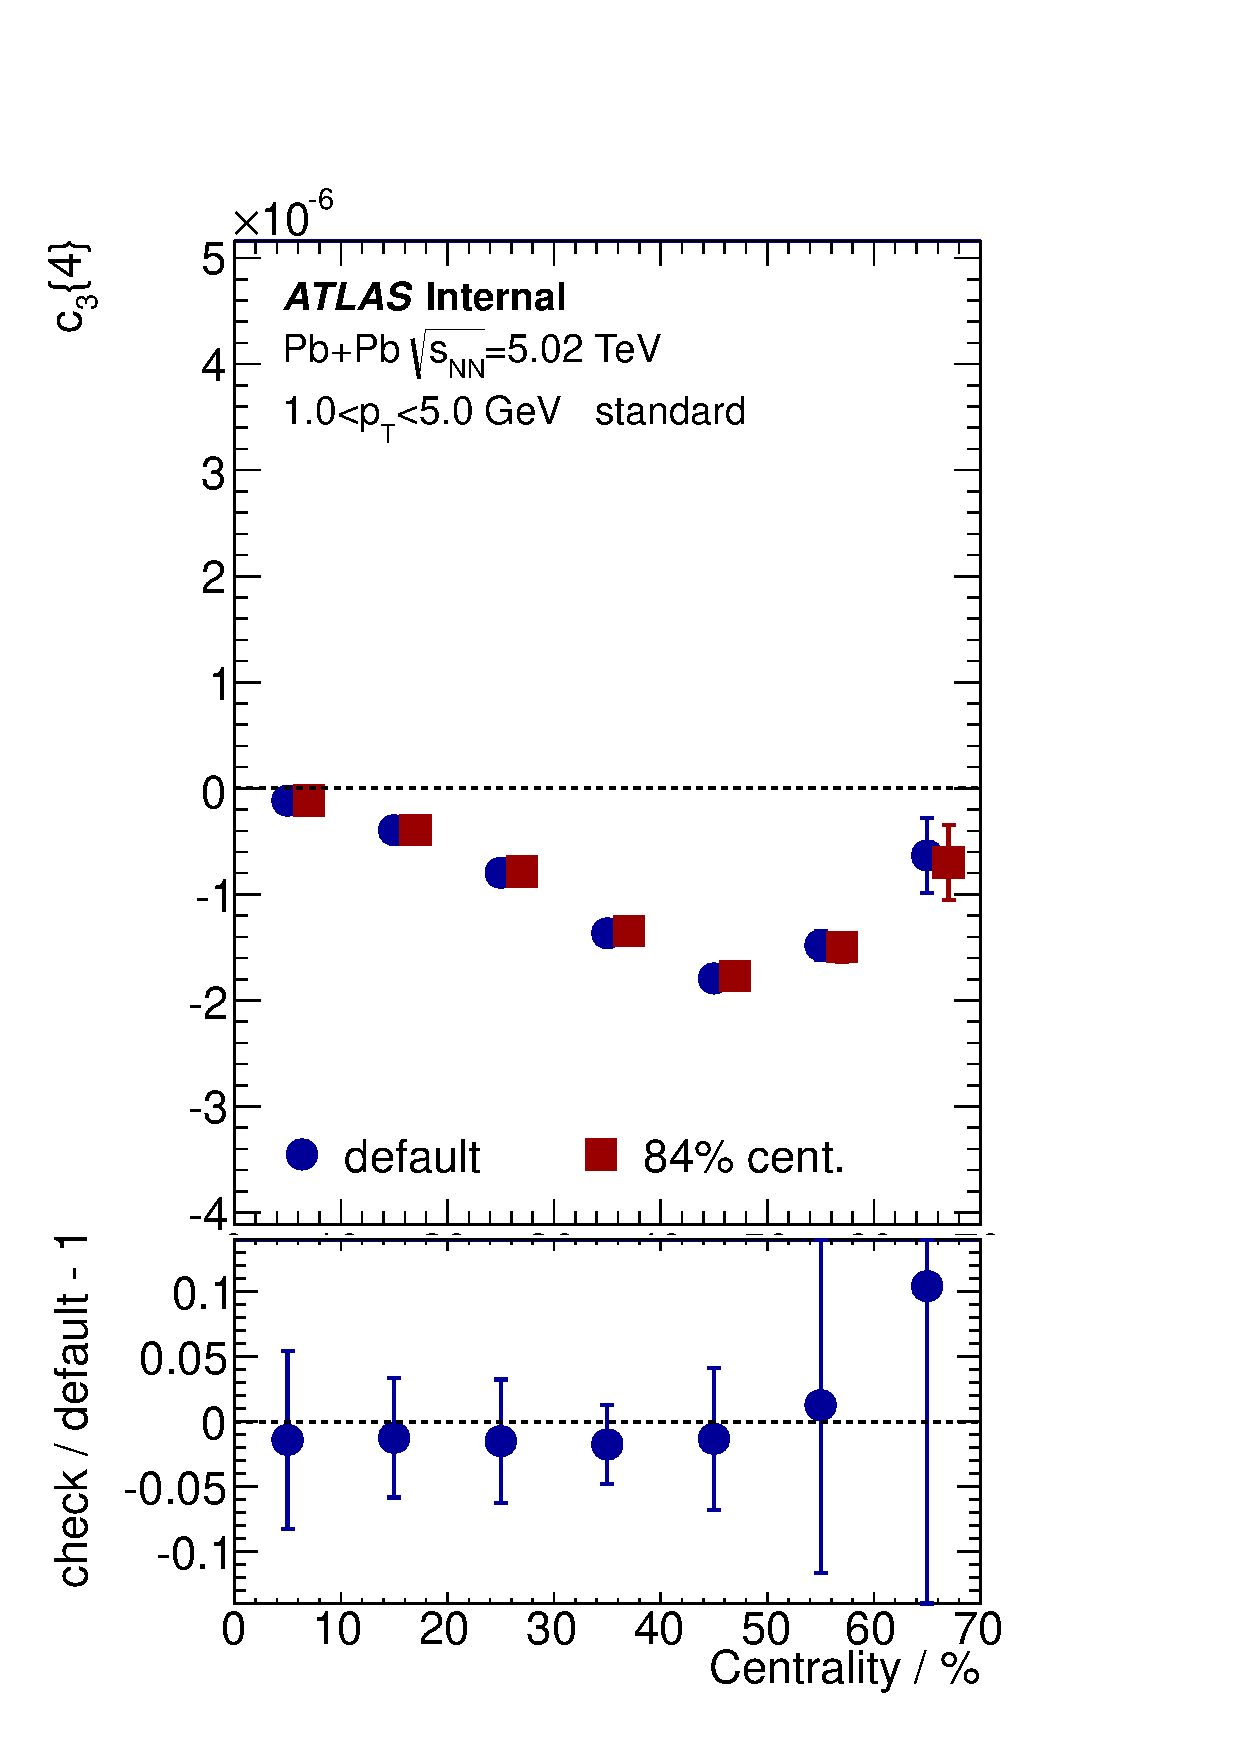
\includegraphics[width=.245\linewidth]{figs/sec_sys/summary/sys7_c4_1sub_Har3_Pt1.pdf}
\caption{Systematics of $c_n\{4\}$ from centrality definition: $(0-85)\%$ v.s. $(0-84)\%$ . Bottom panels are the relative uncertainties between the default and check.}
\label{fig:sys_cent}
\end{figure}
Fig.~\ref{fig:sys_cent} compares the $c_n\{4\}$ for the different centrality ranges. This systematic uncertainty depends on the centrality dependence of the observable: if the observable has no centrality dependence, the uncertainty is zero. On the other hand, this uncertainty is large if the observable is strongly dependent of centrality. This explains why this uncertainty for $c_3\{4\}$ is larger than that of $c_2\{4\}$. Different $p_\text{T}$ ranges make little difference since the relative centrality dependence of the observables do not change much.



\subsection{Event class bin width}
As has been discussed in Sec.~\ref{sec:ana}, cumulant is sensitive to the definition of event class, which is associated with the multiplicity fluctuation. In order to suppress the multiplicity fluctuation, while calculating the multi-particle correlation, the events are always binned with $1\%$ centrality bin width, which is sufficient for cumulant-like analysis~\cite{Jia:2017hbm}. However, unlike in small systems, since the non-flow contribution is much smaller in Pb+Pb collisions, different bin widths will not trigger non-flow fluctuations. However, different bin widths could still result in different flow fluctuations, especially when the bin width is too large. So it is worthwhile to check the impact of event class bin width:
\begin{itemize}
\item default: $1\%$ centrality as the event class bin width;
\item check: $5\%$ centrality as the event class bin width;
\end{itemize}

Fig.~\ref{fig:sys_binWidth} shows the comparison of $c_n\{4\}$ calculated with two event class bin widths. For the lower harmonics $c_1\{4\}$ and $c_2\{4\}$, the relative differences are within statistics errors. While for the higher order harmonics $c_3\{4\}$ and $c_4\{4\}$, since flow signal is smaller, the flow fluctuation becomes larger. This explains why the relative differences of $c_3\{4\}$ and $c_4\{4\}$ between two event class bin widths are larger. This cross-check illustrates the importance of narrow bin width in the cumulant calculation, but it will NOT be quoted as part of the systematics since we will always use the narrowest bin width.
\begin{figure}[H]
\centering
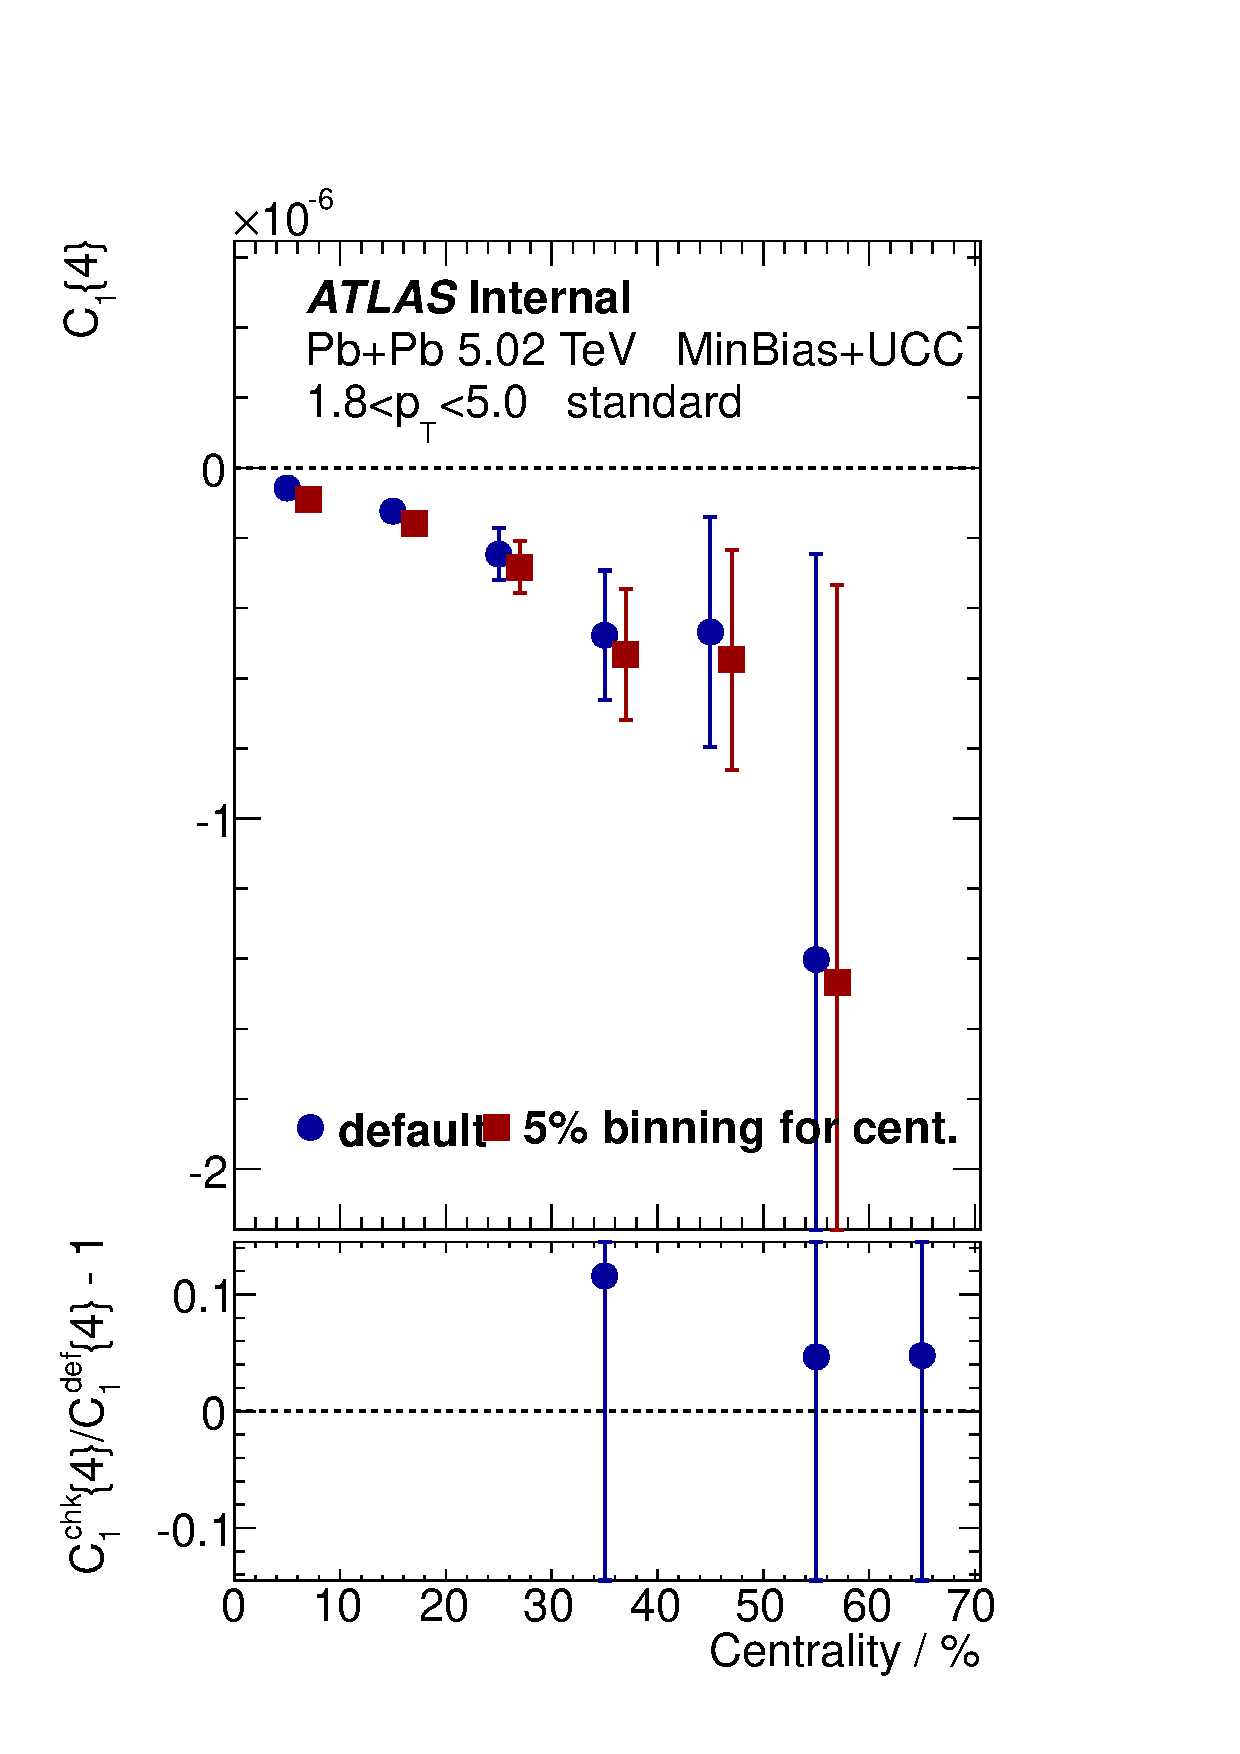
\includegraphics[width=.245\linewidth]{figs/sec_appendix/sys_PbPb502/PbPb502_sys6_1sub_Har1_Pt5.pdf}
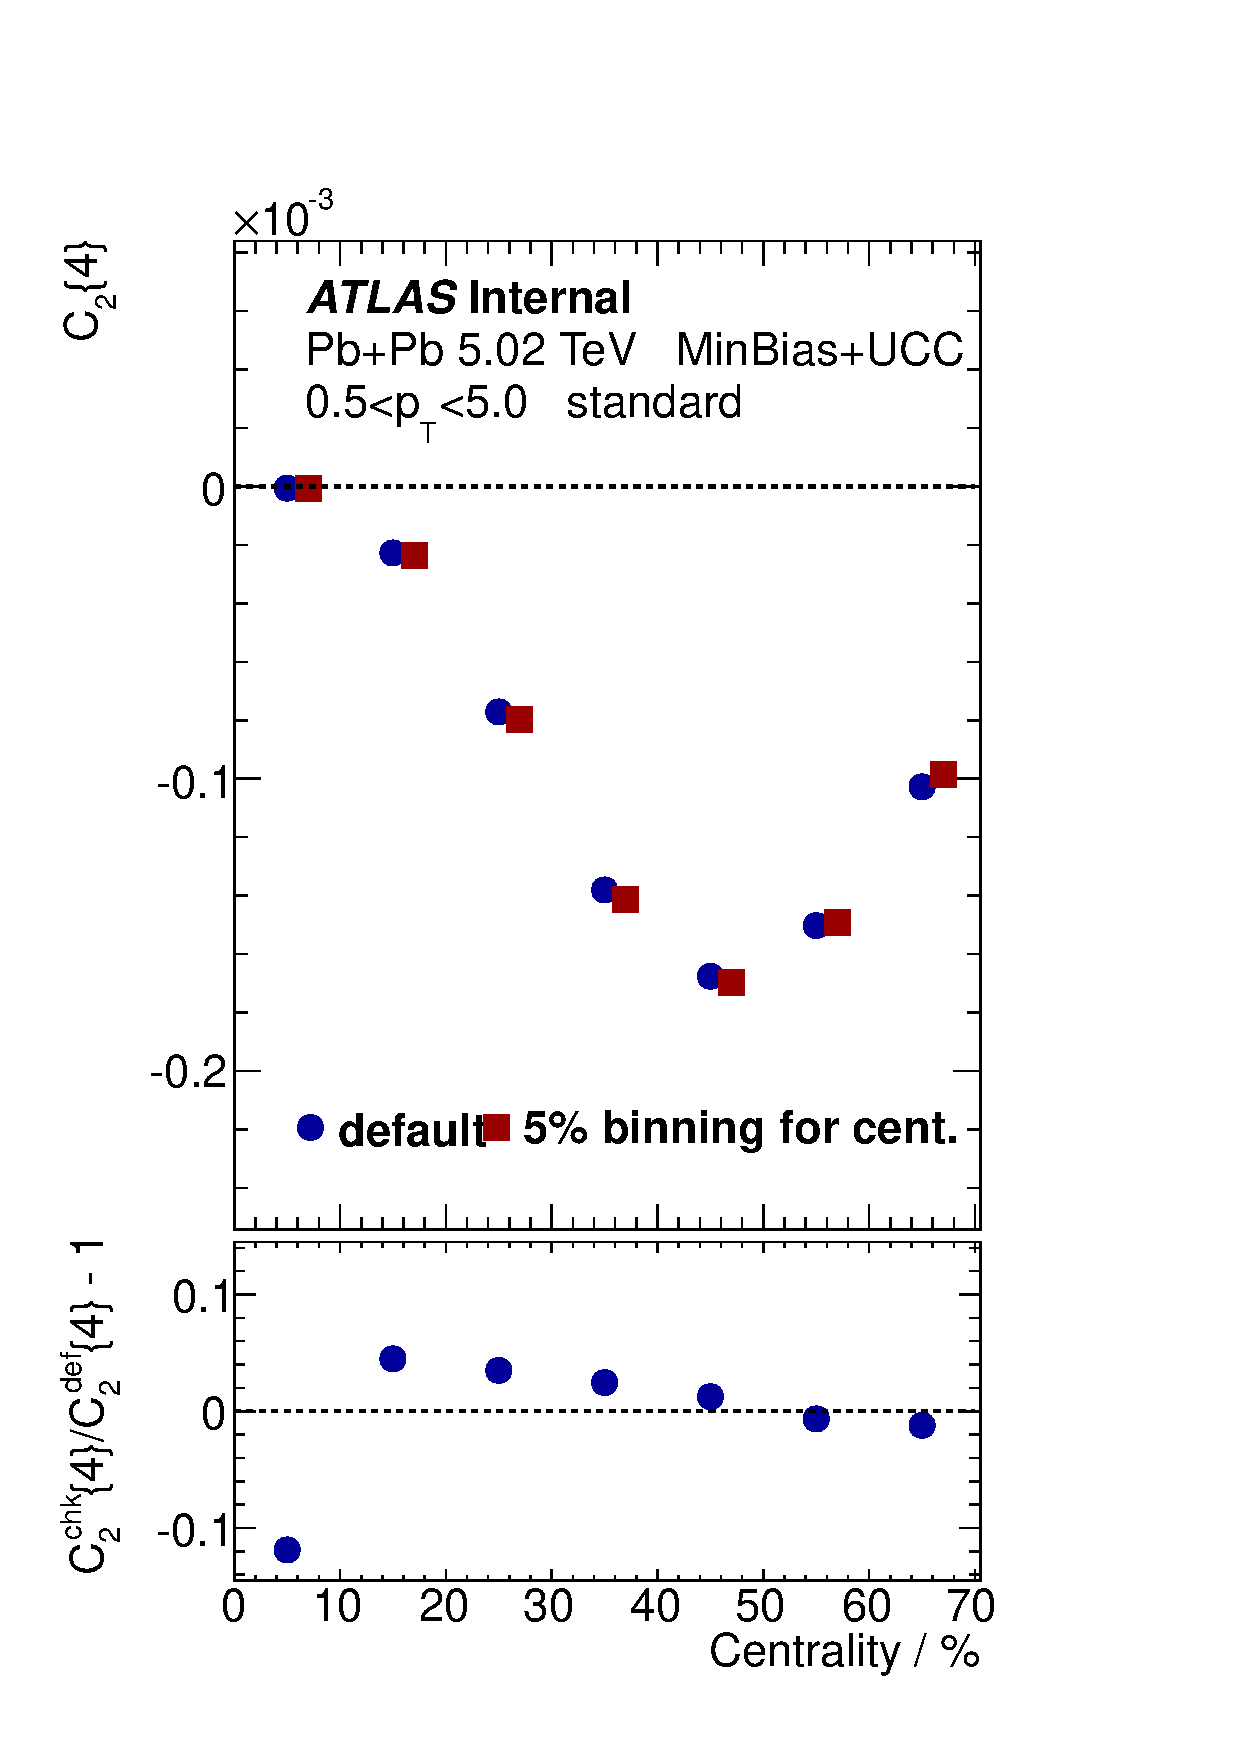
\includegraphics[width=.245\linewidth]{figs/sec_appendix/sys_PbPb502/PbPb502_sys6_1sub_Har2_Pt0.pdf}
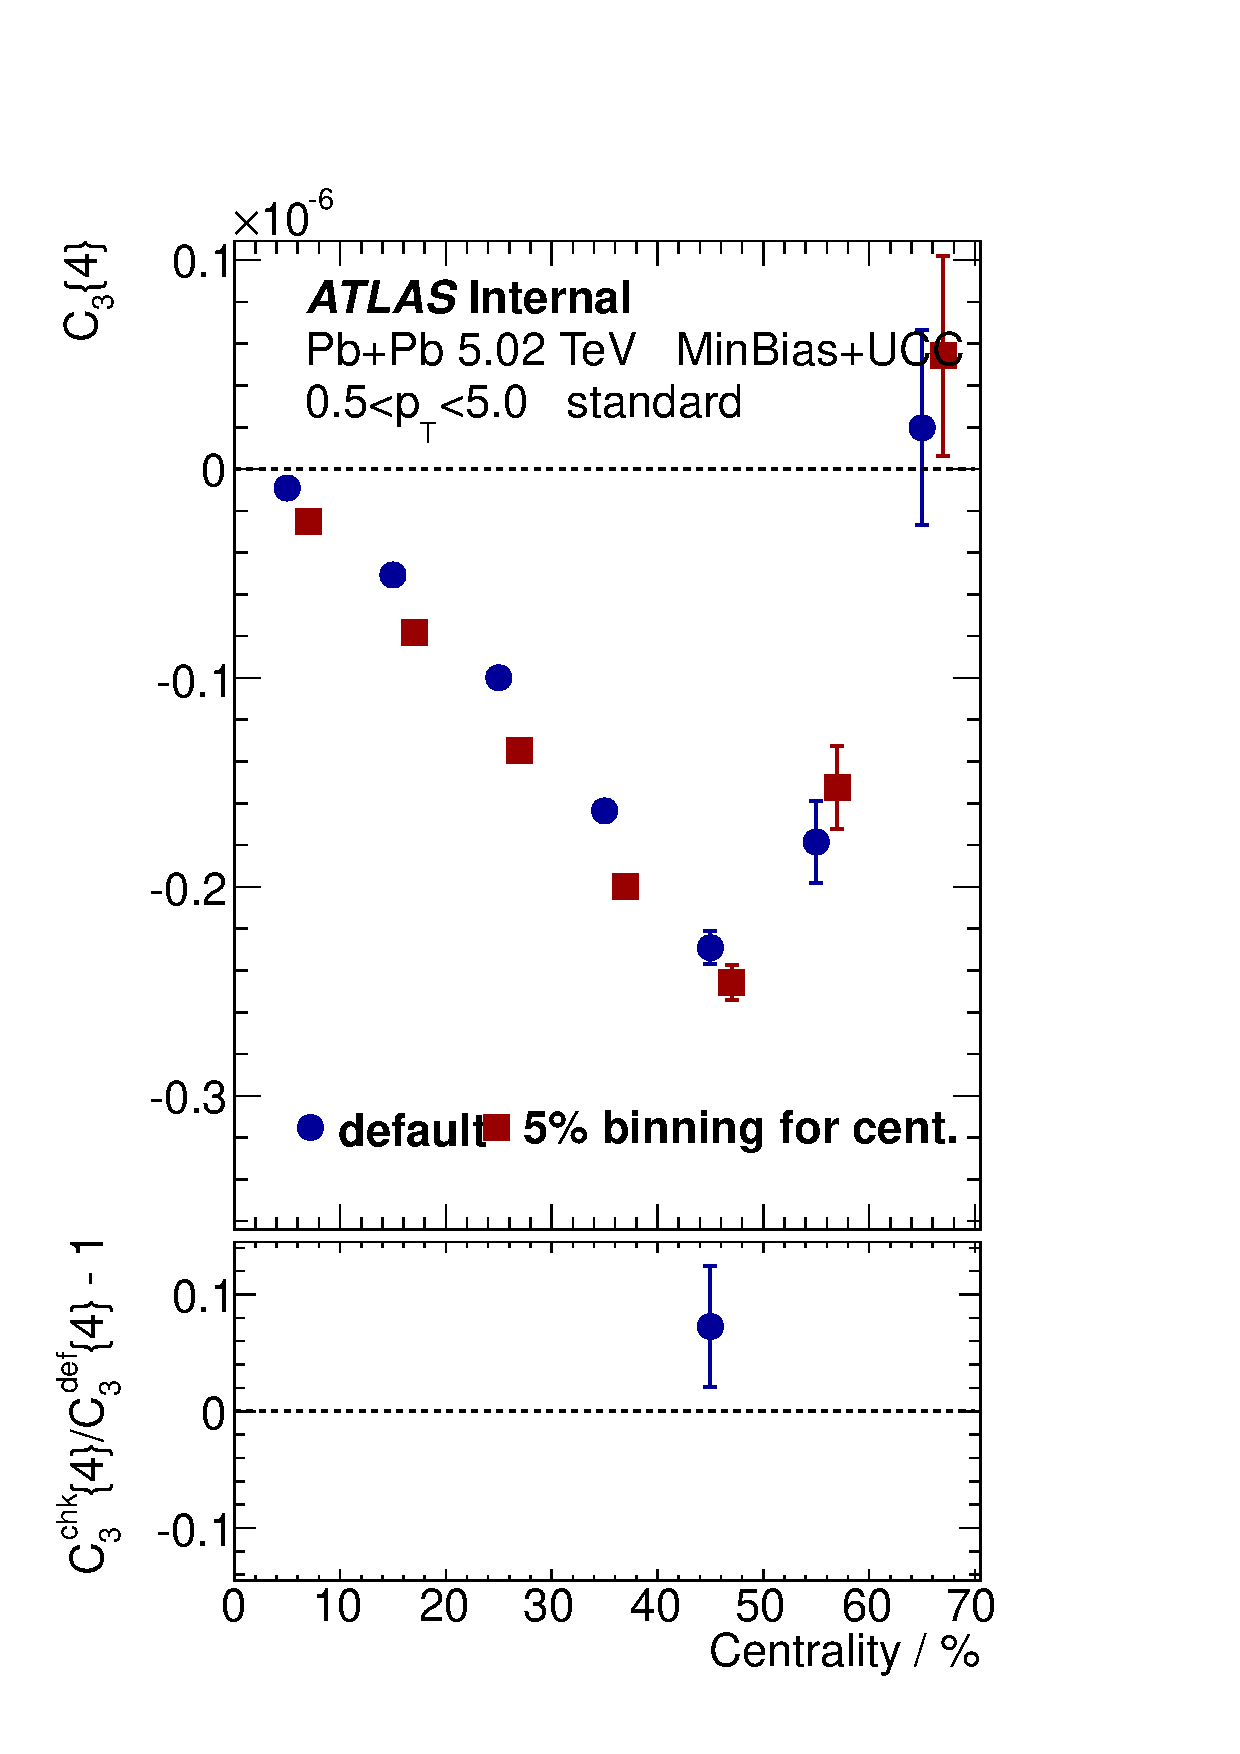
\includegraphics[width=.245\linewidth]{figs/sec_appendix/sys_PbPb502/PbPb502_sys6_1sub_Har3_Pt0.pdf}
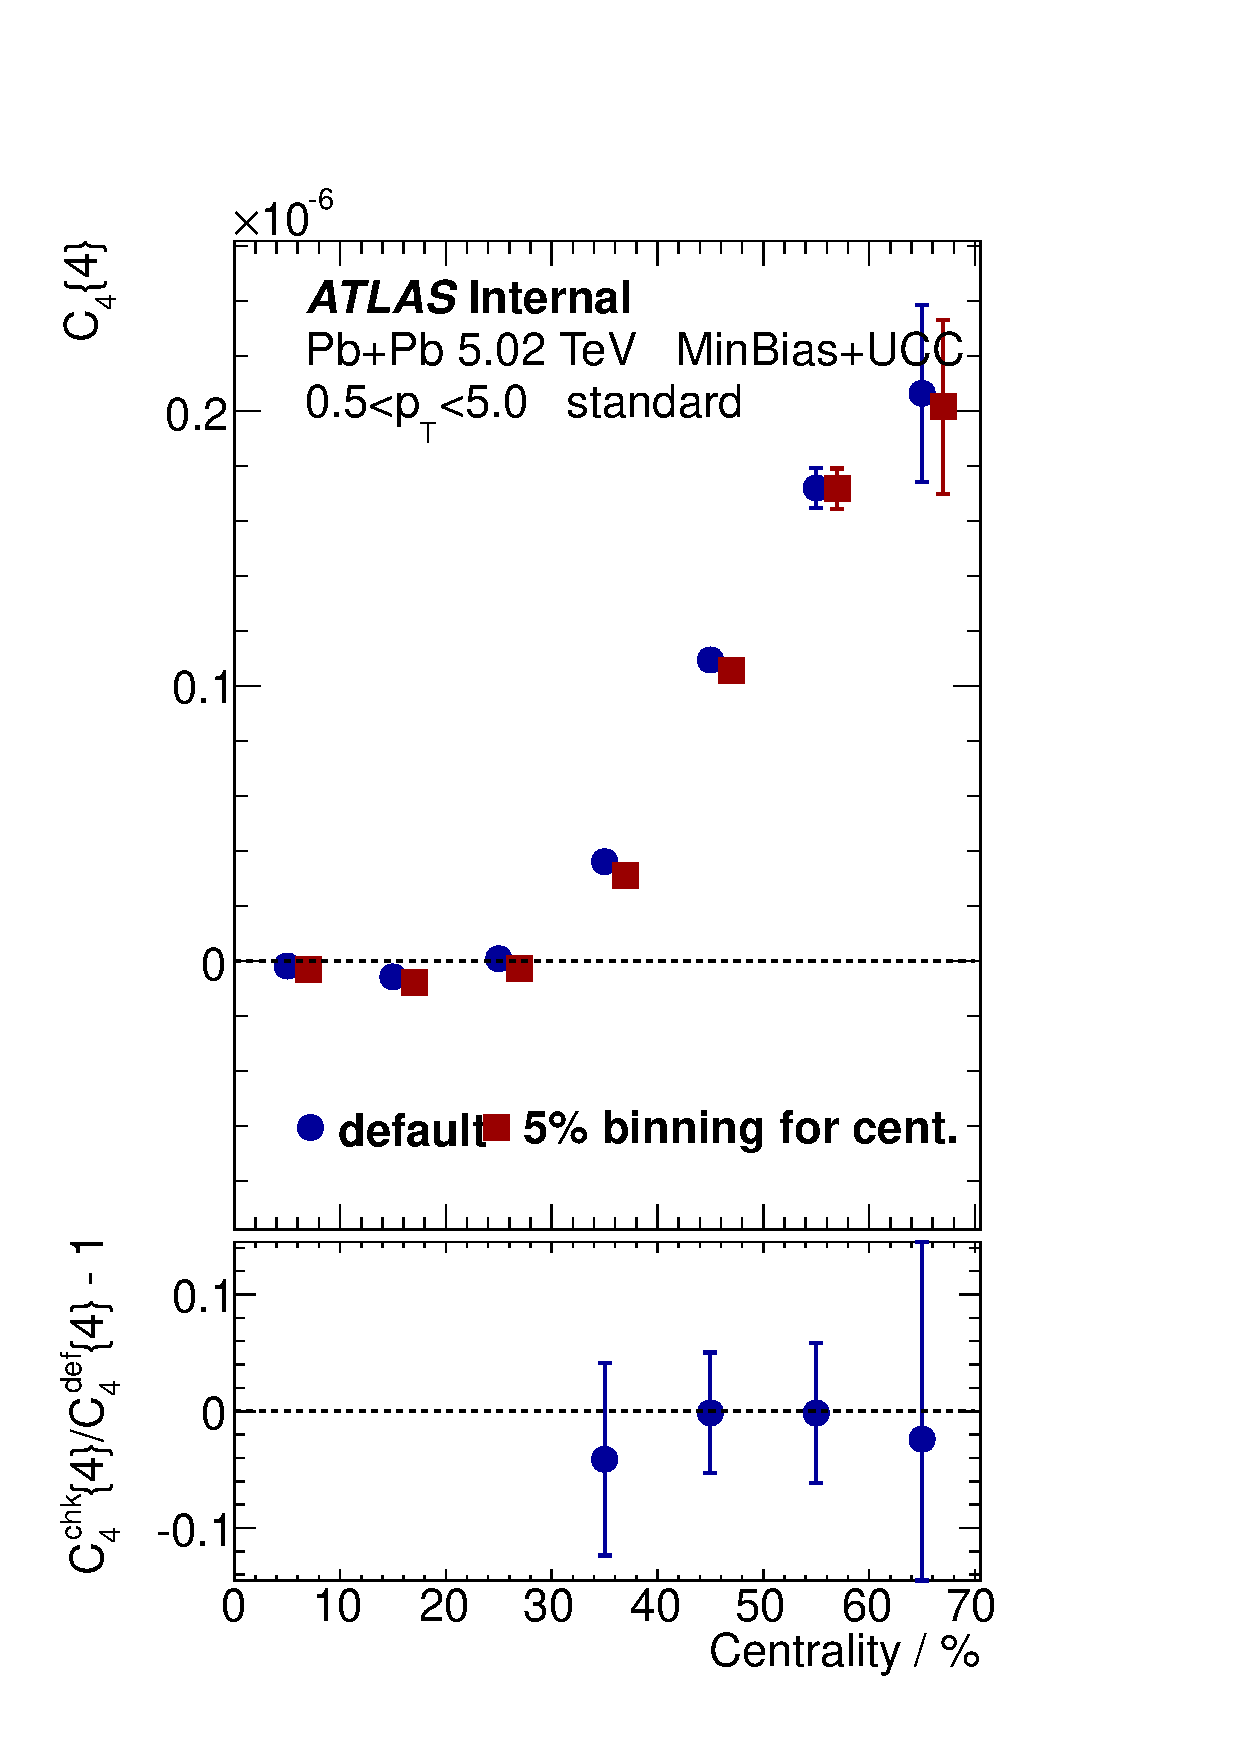
\includegraphics[width=.245\linewidth]{figs/sec_appendix/sys_PbPb502/PbPb502_sys6_1sub_Har4_Pt0.pdf}
\caption{Systematics of $c_n\{4\}$ from different bin width: $1\%$ v.s. $5\%$ centrality bin widths. Bottom panels are the relative uncertainties between the default and check.}
\label{fig:sys_binWidth}
\end{figure}



\subsection{$\eta$ gap for subevent}
Compared with 2-subevent method, 3-subevent method is designed to remove the dijet-like correlation, where the chance that both jets contribute to all the 3 subevents are dramatically lowered. The only situation where dijet correlation still contributes is when two jets fall upon the two boundaries among 3 subevents. To show whether the $c_n\{4\}$ is affected by the residual dijet contributions, we introduced $\eta$ gaps between subevents.

Fig.~\ref{fig:sys_etaGap_eg} is a cartoon showing how the $\eta$ gap was applied to the subevent methods. For the standard cumulant method, in principle $\eta$ gap can also be applied among all 4 particles. However, the formula of direct cumulant will no longer hold and one has to rely on the nested loop method. Meanwhile for the subevent methods, it is quite natural to apply the $\eta$ gaps between subevents, while keeping the formula the same. In the following cross-checks, we will only test the $\eta$ gap in subevent methods. After all, the subevent method is used to evaluate the residual non-flow in Pb+Pb, and if subevent cumulant with $\eta$ gap gives consistent results, it means most of the dijet-like non-flow are already removed by the 3-subevent method.

\begin{figure}[H]
\centering
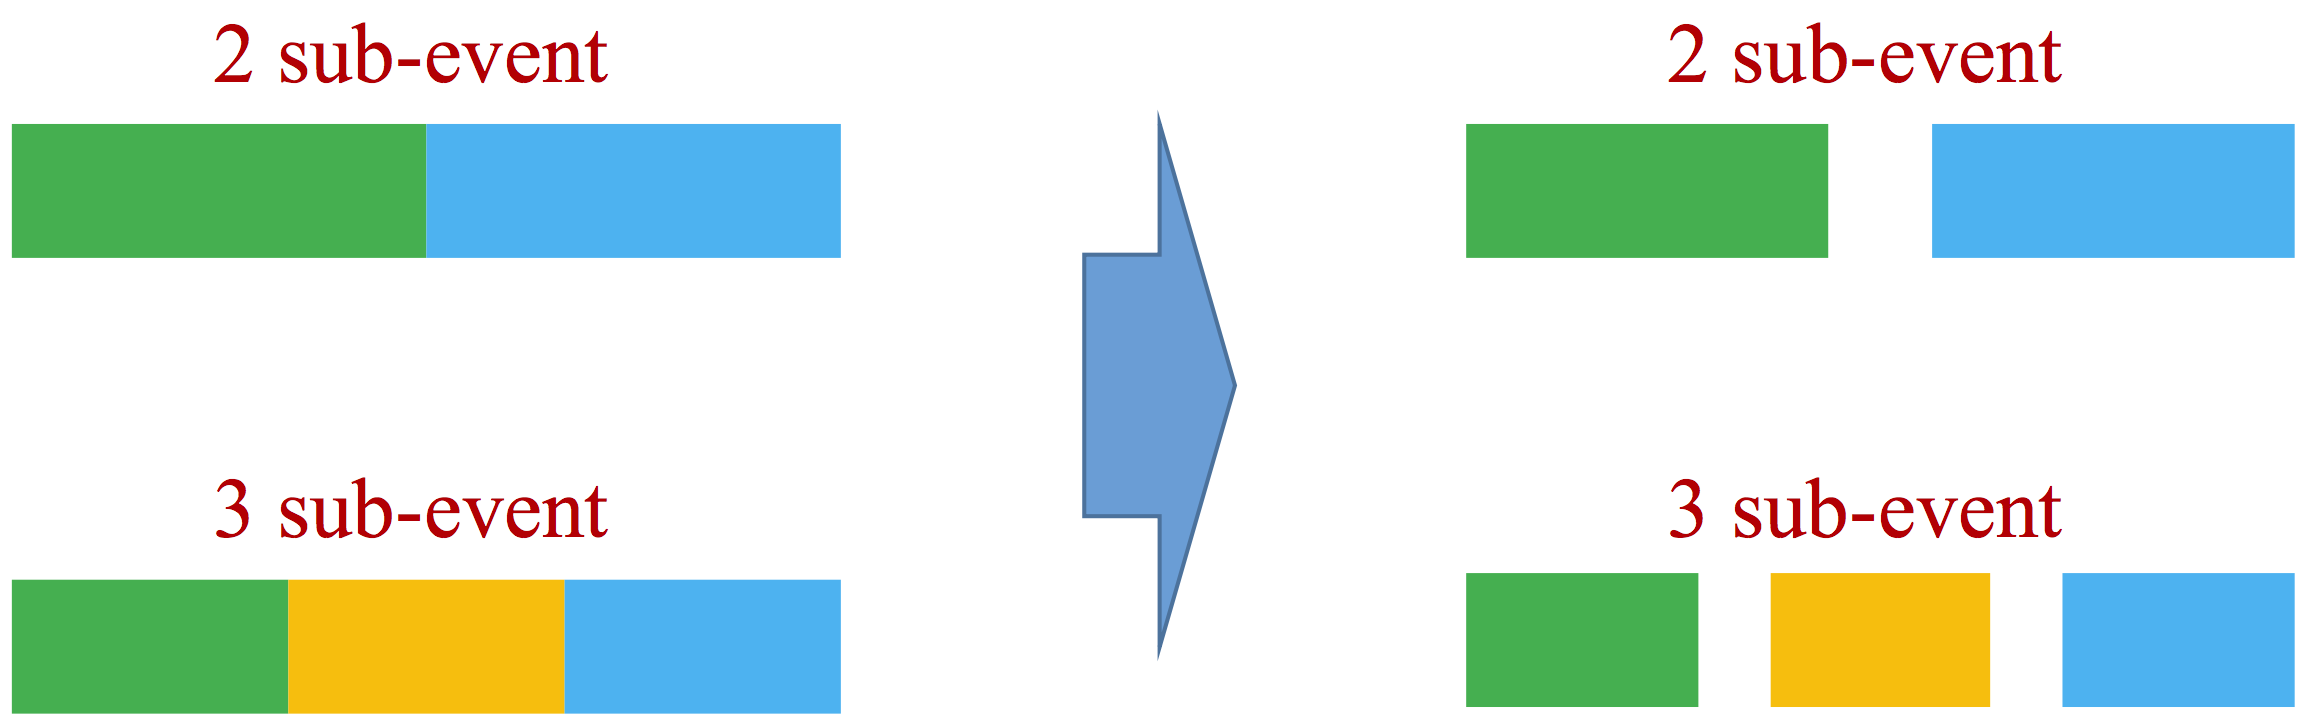
\includegraphics[width=.9\linewidth]{figs/sec_sys/etaGap_eg.png}
\caption{A cartoon showing how the $\eta$ gap was applied to subevent to further suppress the long-range non-flow.}
\label{fig:sys_etaGap_eg}
\end{figure}

Fig.~\ref{fig:sys_etaGap} presents the comparisons of $c_n\{4\}$ with and without $\eta=0.5$ gap, calculated using 3-subevent methods. For $c_2\{4\}$, since the elliptic flow is dominating over the non-flow, applying $\eta$ gap has minimal impact on the results. While for $c_3\{4\}$ and $c_4\{4\}$, where the flow signals become smaller, subevent with $\eta$ gap causes up to $10\%$ difference compared with no gap. In the end, since $c_1\{4\}$ signal is even smaller, by applying the $\eta$ gap, the number of particle combinations in $\lr{4}$ will drop, which results in larger statistical errors. Since the residual non-flow upon subevent cumulant is under control, this cross-check will NOT be quoted as systematics. To increase statistical significance, the default subevent method will NOT include the $\eta$ gap.
\begin{figure}[H]
\centering
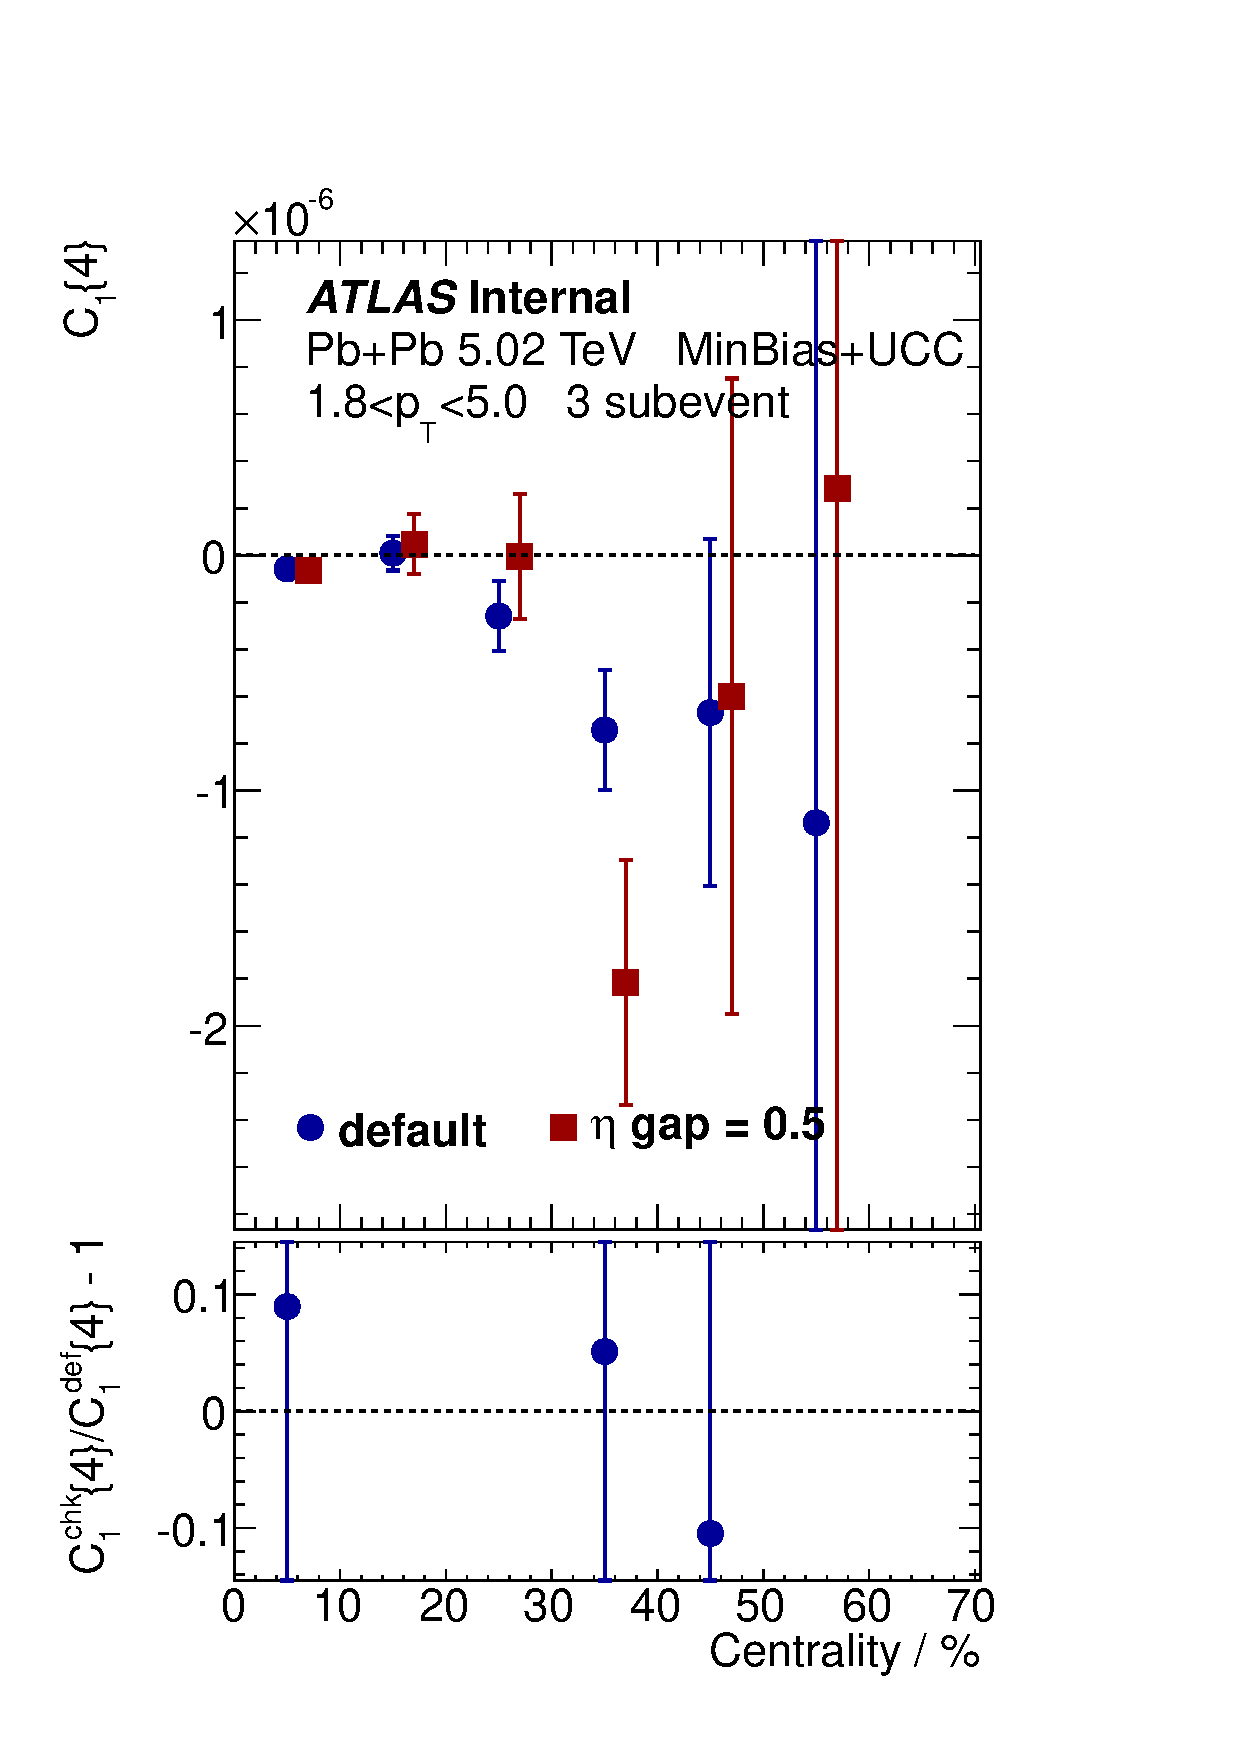
\includegraphics[width=.245\linewidth]{figs/sec_appendix/sys_PbPb502/PbPb502_sys7_3sub_Har1_Pt5.pdf}
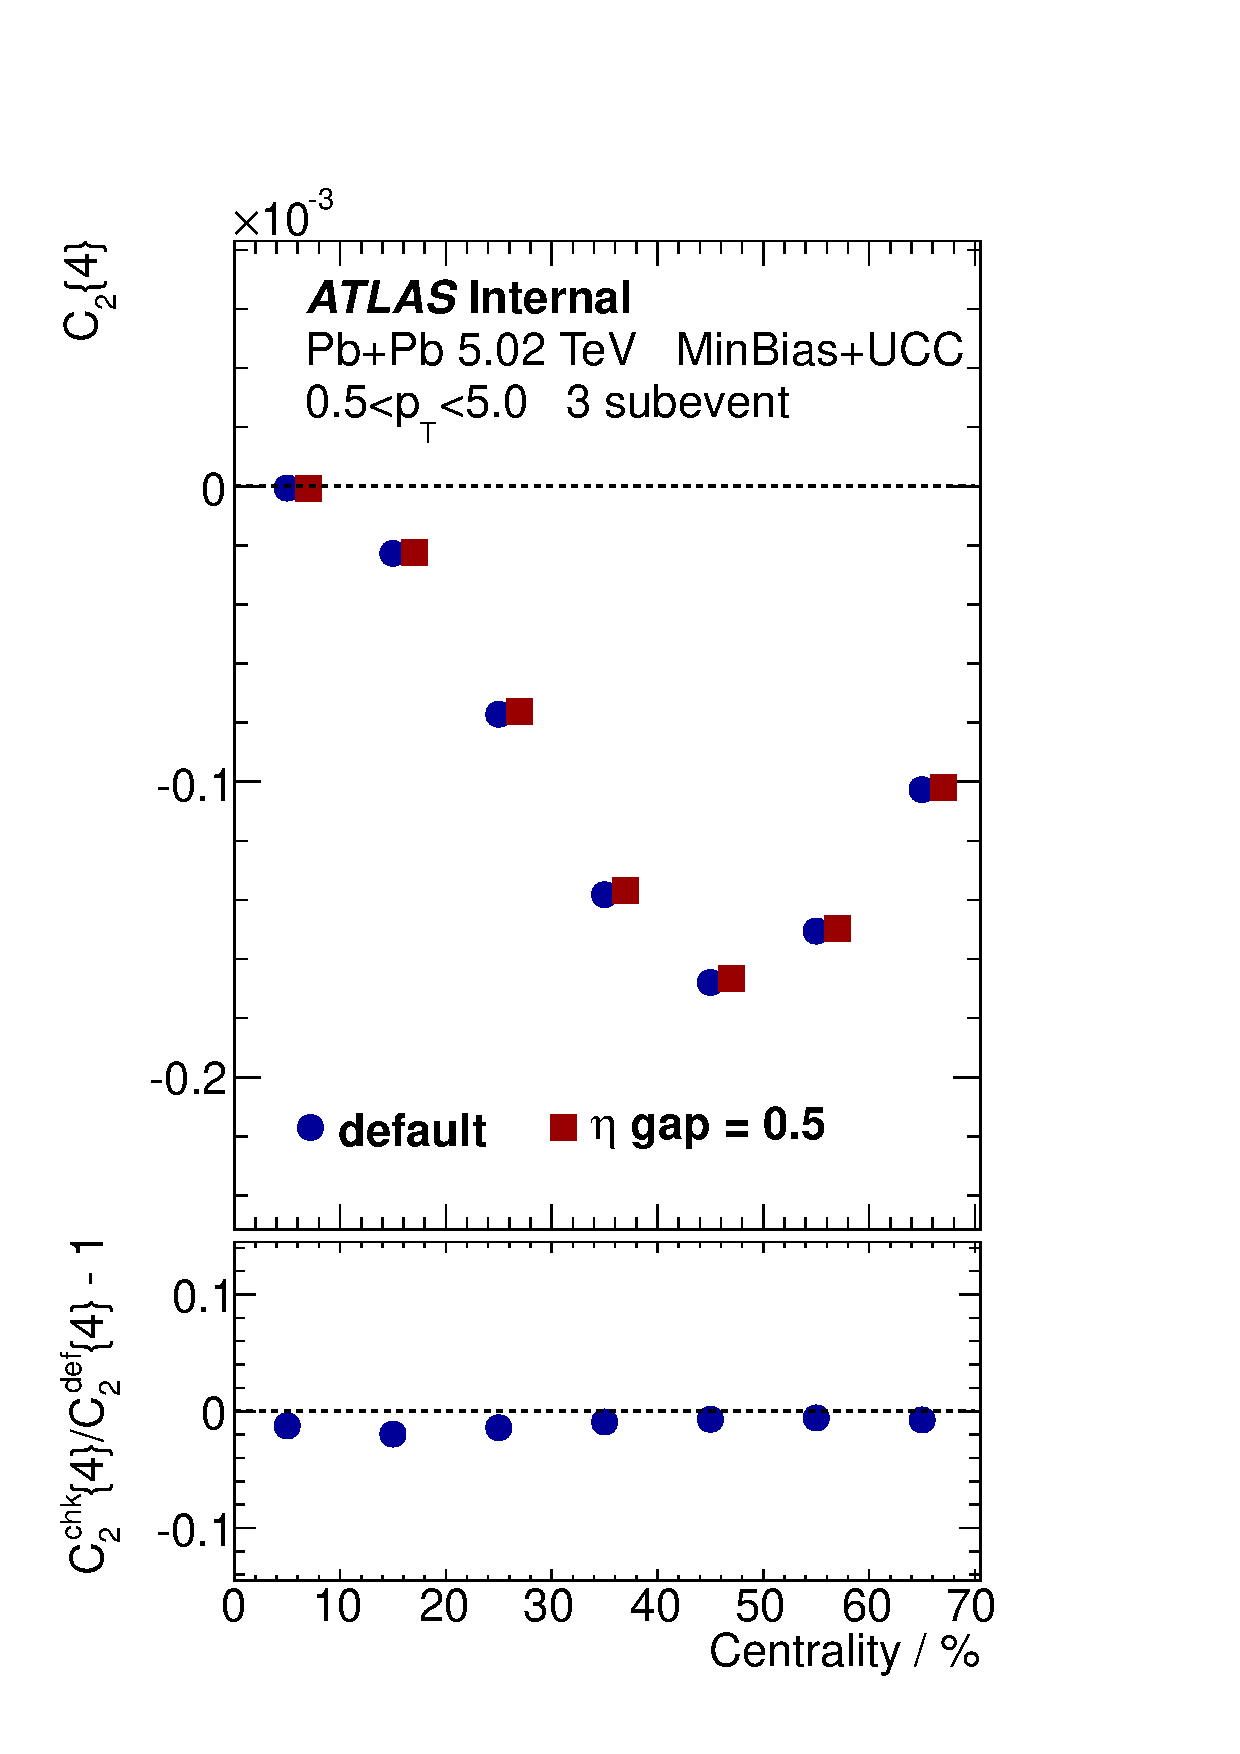
\includegraphics[width=.245\linewidth]{figs/sec_appendix/sys_PbPb502/PbPb502_sys7_3sub_Har2_Pt0.pdf}
\includegraphics[width=.245\linewidth]{figs/sec_appendix/sys_PbPb502/PbPb502_sys7_3sub_Har3_Pt0.pdf}
\includegraphics[width=.245\linewidth]{figs/sec_appendix/sys_PbPb502/PbPb502_sys7_3sub_Har4_Pt0.pdf}
\caption{Systematics of $c_n\{4\}$ from $\eta$ gap between subevents: with $\eta=0.5$ gap and without gap. The $c_n\{4\}$ are calculated using 3-subevent method. Bottom panels are the relative uncertainties between the default and check.}
\label{fig:sys_etaGap}
\end{figure}



\subsection{Summary of systematics}
This section summarizes the breakdown of systematics for every observable in this analysis. In order not to flooding the plots, the results are shown in two $p_\text{T}$ ranges:
\begin{itemize}
\item $0.5<p_\text{T}<5.0$ GeV;
\item $1.0<p_\text{T}<5.0$ GeV;
\end{itemize}
and except for the 2-particle cumulant, all other results are only shown using standard cumulant method. The corresponding systematics from 3-subevent method is listed in the Appendix.

Overall, the summary of systematics has the following features:
\begin{itemize}
\item In most cases, systematics are dominated by tracking efficiency variations. This is not surprising since magnitude of flow, as well as its fluctuation, are highly dependent of $p_\text{T}$. Slightly change in tracking efficiency as a function of $p_\text{T}$ will cause noticeable differences to cumulants;
\item Monte-Carlo closure has significant impact on $c_n\{2k\}$: in the lower $p_\text{T}$ region, about $5\%$ for 2-particle cumulant, $10\%$ and $15\%$ for 4- and 6-particle cumulants. In higher $p_\text{T}$, systematics from MC closure become much smaller;
\item Normalized cumulant, symmetric cumulant and asymmetric cumulant have smaller systematic errors than its correspondence without normalization, due to the reason that part of the systematics are canceled out in the ratio;
\end{itemize}

As a summary, in most cases, the total systematics are within $10\%$. In other cases where the systematics are larger, they are still smaller or comparable with statistical uncertainties.

\subsubsection{2-particle cumulant $c_n\{2\}$}
\begin{figure}[H]
\centering
\includegraphics[width=.425\linewidth]{figs/sec_sys/summary/sys_c2_3sub_Har2_Pt0.pdf}
\includegraphics[width=.425\linewidth]{figs/sec_sys/summary/sys_c2_3sub_Har2_Pt1.pdf}
\includegraphics[width=.425\linewidth]{figs/sec_sys/summary/sys_c2_3sub_Har3_Pt0.pdf}
\includegraphics[width=.425\linewidth]{figs/sec_sys/summary/sys_c2_3sub_Har3_Pt1.pdf}
\includegraphics[width=.425\linewidth]{figs/sec_sys/summary/sys_c2_3sub_Har4_Pt0.pdf}
\includegraphics[width=.425\linewidth]{figs/sec_sys/summary/sys_c2_3sub_Har4_Pt1.pdf}
\caption{Breakdown of all major systematic sources for 2-particle cumulant $c_n\{2\}$. Left column shows the lower $p_\text{T}$ cut and right column shows the higher $p_\text{T}$ cut. Different rows represent different harmonics. The cumulants are calculated using standard method. Shaded area indicate the statistical uncertainty.}
\label{fig:sys_sum_c2}
\end{figure}

\subsubsection{4-particle cumulant $c_n\{4\}$ and $\hat{c}_n\{4\}$}
\begin{figure}[H]
\centering
\includegraphics[width=.425\linewidth]{figs/sec_sys/summary/sys_c4_1sub_Har2_Pt0.pdf}
\includegraphics[width=.425\linewidth]{figs/sec_sys/summary/sys_c4_1sub_Har2_Pt1.pdf}
\includegraphics[width=.425\linewidth]{figs/sec_sys/summary/sys_c4_1sub_Har3_Pt0.pdf}
\includegraphics[width=.425\linewidth]{figs/sec_sys/summary/sys_c4_1sub_Har3_Pt1.pdf}
\includegraphics[width=.425\linewidth]{figs/sec_sys/summary/sys_c4_1sub_Har4_Pt0.pdf}
\includegraphics[width=.425\linewidth]{figs/sec_sys/summary/sys_c4_1sub_Har4_Pt1.pdf}
\caption{Breakdown of all major systematic sources for 4-particle cumulant $c_n\{4\}$. Left column shows the lower $p_\text{T}$ cut and right column shows the higher $p_\text{T}$ cut. Different rows represent different harmonics. The cumulants are calculated using standard method. Shaded area indicate the statistical uncertainty.}
\label{fig:sys_sum_c4}
\end{figure}

\begin{figure}[H]
\centering
\includegraphics[width=.425\linewidth]{figs/sec_sys/summary/sys_nc4_1sub_Har2_Pt0.pdf}
\includegraphics[width=.425\linewidth]{figs/sec_sys/summary/sys_nc4_1sub_Har2_Pt1.pdf}
\includegraphics[width=.425\linewidth]{figs/sec_sys/summary/sys_nc4_1sub_Har3_Pt0.pdf}
\includegraphics[width=.425\linewidth]{figs/sec_sys/summary/sys_nc4_1sub_Har3_Pt1.pdf}
\includegraphics[width=.425\linewidth]{figs/sec_sys/summary/sys_nc4_1sub_Har4_Pt0.pdf}
\includegraphics[width=.425\linewidth]{figs/sec_sys/summary/sys_nc4_1sub_Har4_Pt1.pdf}
\caption{Breakdown of all major systematic sources for normalized 4-particle cumulant $\hat{c}_n\{4\}$. Left column shows the lower $p_\text{T}$ cut and right column shows the higher $p_\text{T}$ cut. Different rows represent different harmonics. The cumulants are calculated using standard method. Shaded area indicate the statistical uncertainty.}
\label{fig:sys_sum_nc4}
\end{figure}

\subsubsection{6-particle cumulant $c_n\{6\}$ and $\hat{c}_n\{6\}$}
\begin{figure}[H]
\centering
\includegraphics[width=.425\linewidth]{figs/sec_sys/summary/sys_c6_1sub_Har2_Pt0.pdf}
\includegraphics[width=.425\linewidth]{figs/sec_sys/summary/sys_c6_1sub_Har2_Pt1.pdf}
\includegraphics[width=.425\linewidth]{figs/sec_sys/summary/sys_c6_1sub_Har3_Pt0.pdf}
\includegraphics[width=.425\linewidth]{figs/sec_sys/summary/sys_c6_1sub_Har3_Pt1.pdf}
\includegraphics[width=.425\linewidth]{figs/sec_sys/summary/sys_c6_1sub_Har4_Pt0.pdf}
\includegraphics[width=.425\linewidth]{figs/sec_sys/summary/sys_c6_1sub_Har4_Pt1.pdf}
\caption{Breakdown of all major systematic sources for 6-particle cumulant $c_n\{6\}$. Left column shows the lower $p_\text{T}$ cut and right column shows the higher $p_\text{T}$ cut. Different rows represent different harmonics. The cumulants are calculated using standard method. Shaded area indicate the statistical uncertainty.}
\label{fig:sys_sum_c6}
\end{figure}

\begin{figure}[H]
\centering
\includegraphics[width=.425\linewidth]{figs/sec_sys/summary/sys_nc6_1sub_Har2_Pt0.pdf}
\includegraphics[width=.425\linewidth]{figs/sec_sys/summary/sys_nc6_1sub_Har2_Pt1.pdf}
\includegraphics[width=.425\linewidth]{figs/sec_sys/summary/sys_nc6_1sub_Har3_Pt0.pdf}
\includegraphics[width=.425\linewidth]{figs/sec_sys/summary/sys_nc6_1sub_Har3_Pt1.pdf}
\includegraphics[width=.425\linewidth]{figs/sec_sys/summary/sys_nc6_1sub_Har4_Pt0.pdf}
\includegraphics[width=.425\linewidth]{figs/sec_sys/summary/sys_nc6_1sub_Har4_Pt1.pdf}
\caption{Breakdown of all major systematic sources for normalized 6-particle cumulant $\hat{c}_n\{6\}$. Left column shows the lower $p_\text{T}$ cut and right column shows the higher $p_\text{T}$ cut. Different rows represent different harmonics. The cumulants are calculated using standard method. Shaded area indicate the statistical uncertainty.}
\label{fig:sys_sum_nc6}
\end{figure}

\subsubsection{Universality check of flow fluctuation}
\begin{figure}[H]
\centering
\includegraphics[width=.425\linewidth]{figs/sec_sys/summary/sys_isGauss_1sub_Har2_Pt0.pdf}
\includegraphics[width=.425\linewidth]{figs/sec_sys/summary/sys_isGauss_1sub_Har2_Pt1.pdf}
\includegraphics[width=.425\linewidth]{figs/sec_sys/summary/sys_isPower_1sub_Har2_Pt0.pdf}
\includegraphics[width=.425\linewidth]{figs/sec_sys/summary/sys_isPower_1sub_Har2_Pt1.pdf}
\caption{Breakdown of all major systematic sources for flow fluctuation check. Left column shows the lower $p_\text{T}$ cut and right column shows the higher $p_\text{T}$ cut. Different rows represent different fluctuation models. The cumulants are calculated using standard method. Shaded area indicate the statistical uncertainty.}
\label{fig:sys_sum_fluc}
\end{figure}

\subsubsection{Symmetric and normalized symmetric cumulant $sc_{n,m}\{4\}$ and $nsc_{n,m}\{4\}$}
\begin{figure}[H]
\centering
\includegraphics[width=.425\linewidth]{figs/sec_sys/summary/sys_sc_1sub_Har2_Pt0.pdf}
\includegraphics[width=.425\linewidth]{figs/sec_sys/summary/sys_sc_1sub_Har2_Pt1.pdf}
\includegraphics[width=.425\linewidth]{figs/sec_sys/summary/sys_sc_1sub_Har3_Pt0.pdf}
\includegraphics[width=.425\linewidth]{figs/sec_sys/summary/sys_sc_1sub_Har3_Pt1.pdf}
\caption{Breakdown of all major systematic sources for symmetric cumulant $sc_{n,m}\{4\}$. Left column shows the lower $p_\text{T}$ cut and right column shows the higher $p_\text{T}$ cut. Different rows represent different harmonic combinations. The cumulants are calculated using standard method. Shaded area indicate the statistical uncertainty.}
\label{fig:sys_sum_sc}
\end{figure}

\begin{figure}[H]
\centering
\includegraphics[width=.425\linewidth]{figs/sec_sys/summary/sys_nsc_1sub_Har2_Pt0.pdf}
\includegraphics[width=.425\linewidth]{figs/sec_sys/summary/sys_nsc_1sub_Har2_Pt1.pdf}
\includegraphics[width=.425\linewidth]{figs/sec_sys/summary/sys_nsc_1sub_Har3_Pt0.pdf}
\includegraphics[width=.425\linewidth]{figs/sec_sys/summary/sys_nsc_1sub_Har3_Pt1.pdf}
\caption{Breakdown of all major systematic sources for normalized symmetric cumulant $nsc_{n,m}\{4\}$. Left column shows the lower $p_\text{T}$ cut and right column shows the higher $p_\text{T}$ cut. Different rows represent different harmonic combinations. The cumulants are calculated using standard method. Shaded area indicate the statistical uncertainty.}
\label{fig:sys_sum_nsc}
\end{figure}

\subsubsection{Asymmetric and normalized asymmetric cumulant $ac_{n,n+m}\{3\}$ and $nac_{n,n+m}\{3\}$}
\begin{figure}[H]
\centering
\includegraphics[width=.425\linewidth]{figs/sec_sys/summary/sys_ac_1sub_Har2_Pt0.pdf}
\includegraphics[width=.425\linewidth]{figs/sec_sys/summary/sys_ac_1sub_Har2_Pt1.pdf}
\caption{Breakdown of all major systematic sources for asymmetric cumulant $ac_{n,n+m}\{3\}$. Left column shows the lower $p_\text{T}$ cut and right column shows the higher $p_\text{T}$ cut. The cumulants are calculated using standard method. Shaded area indicate the statistical uncertainty.}
\label{fig:sys_sum_ac}
\end{figure}

\begin{figure}[H]
\centering
\includegraphics[width=.425\linewidth]{figs/sec_sys/summary/sys_nac_1sub_Har2_Pt0.pdf}
\includegraphics[width=.425\linewidth]{figs/sec_sys/summary/sys_nac_1sub_Har2_Pt1.pdf}
\caption{Breakdown of all major systematic sources for normalized asymmetric cumulant $nac_{n,n+m}\{3\}$. Left column shows the lower $p_\text{T}$ cut and right column shows the higher $p_\text{T}$ cut. The cumulants are calculated using standard method. Shaded area indicate the statistical uncertainty.}
\label{fig:sys_sum_nac}
\end{figure}






